%---------------------------------------------------------------------
%
% Chapter 6: Empirical Analysis On Grid Problems
%
%---------------------------------------------------------------------
%
% ChapEmpiricalAnalysisGrids.tex
% Copyright 2015 Dr. Francisco J. Pulido
%
% This file belongs to the PhD titled "New Techniques and Algorithms for Multiobjective and Lexicographic Goal-Based Shortest Path Problems", distributed under the Creative Commons Licence Attribution-NonCommercial-NoDerivs 3.0, available in http://creativecommons.org/licenses/by-nc-nd/3.0/. The complete PhD dissertation is freely accessible from http://www.lcc.uma.es/~francis/
%
% This thesis has been written adapting the TeXiS template, a LaTeX template for writting thesis and other documents. The complete TeXiS package can be obtained from http://gaia.fdi.ucm.es/projects/texis/. TeXis is distributed under the same conditions of the LaTeX Project Public License (http://www.latex-project.org/lppl.txt). The complete license is available in http://creativecommons.org/licenses/by-sa/3.0/legalcode
%
%---------------------------------------------------------------------

\chapter{Empirical Analysis on Grid Problems}
\label{chapEmpiricalAnalysisGrids}
%
\begin{FraseCelebre}
\begin{Frase}
It doesn't matter how beautiful your theory is, it doesn't matter how smart you are. If it doesn't agree with experiment, it's wrong.
\end{Frase}
\begin{Fuente}
Richard P. Feynman (1918-1988)
\end{Fuente}
\end{FraseCelebre}
%
%\begin{resumen}
%

One of the main goals of this thesis is to develop efficient procedures for the goal-based search problem. In Chapter \ref{chapContributions} we introduced \lexgo, a new search algorithm for lexicographic goal problems, as well as an improved procedure for efficient dominance checks in multicriteria search algorithms. This procedure can be applied to \lexgo \ and \namoa, yielding algorithms \lexgote \ and \namoate. Formal properties of these algorithms were presented in Chapter \ref{chapFormalAnalysis}. \lexgo \ and \lexgote \ always return the set of all goal-optimal solutions to a lexicographic goal search problem, while \namoate \ returns the set of all Pareto-optimal solutions to a Multiobjective Search Problem.

In this chapter we evaluate experimentally the performance of two different strategies for lexicographic goal problems: (a) use a multiobjective search algorithm (like \namoa \ or \namoate), and then select the goal-optimal solutions among those in the Pareto set, (b) use a specific goal-based algorithm (like \lexgo \ or \lexgote).

First, we shall describe the experimental setup in Section \ref{chapEmpiricalAnalysis:sec:grids}, which is based on the use of randomly generated grid problems with three to five criteria. We analyze time and space performance of the algorithms for problems of increasing depth. We also evaluate performance for different kinds of goal preferences. More precisely, we set up goals that range from unsatisfiability to satisfability by increasingly larger subsets of the Pareto set. Chapter \ref{chapEmpiricalAnalysisRoadMaps} will present additional experiments over route planning problems in realistic road maps.

We perform systematic comparisons between the algorithms. First we compare \lexgo \ against full Pareto search with \namoa \ (using both lexicographic and linear aggregation selection policies in both algorithms) in Section \ref{chapEmpiricalAnalysis:sec:resultsgridslexgo}. Then, we evaluate the algorithms that employ the dimensionality reduction technique against the standard ones. First, we compare in Section \ref{chapEmpiricalAnalysis:sec:resultsgridsnamoate} \namoa \ with a linear aggregation selection policy against our new version \namoate. After that we compare \lexgote \ against \lexgo \ in Section \ref{chapEmpiricalAnalysis:sec:resultsgridslexgote}. Finally, we evaluate both versions that employ t-discarding over problems with goals. A summary and conclusions are presented at the end of this chapter.

%-------------------------------------------------------------------
\section{Experimental setup}
\label{chapEmpiricalAnalysis:sec:grids}
%-------------------------------------------------------------------

This chapter evaluates the performance of algorithms over sets of randomly generated grids. Furthermore, we have generated three uncorrelated criteria in order to evaluate search with goal-based preferences and three to five uncorrelated criteria when we evaluate multiobjective search without preferences (\namoa \ versus \namoate). The solution depth is used as an indicator of problem difficulty. All multiobjective search algorithms analyzed in this thesis employ the ideal point as lower bound (described in Section \ref{chapMultiObjAlg:subsec:tc}). 

We use randomly generated grids which are a standard test bed in the evaluation of multicriteria search algorithms \citep{Machuca2012} \citep{Raith2009a}. Square bi-dimensional grids of $100 \times 100$ nodes with a vicinity of four neighbors were generated as described in Section \ref{chapMultiObjTestBeds:subsec:RandomGrids}. The start node is placed at the grid center and a single destination node is placed in the diagonal from the center to the bottom right corner. Different solution depths are considered, varying from 20 to 100. A set of five different problems was generated for each solution depth. For each arc a vector $\vec c(i,j) = (c_1,c_2,...,c_q)$ of $q$ integer scalar costs was randomly generated in the range [1,10] using an uniform distribution, i.e. leading to uncorrelated objectives.

In order to assess search with goal-based preferences two different classes of experiments were carried out. Three goals grouped in two priority levels were considered, where target values are defined in terms of the ideal and nadir points. The first class of experiments defines five different sets of targets using the constant $k_1 \in \{ 0, 0.25, 0.5, 0.75, 1 \}$ for both priority levels (see Equation \ref{eq:targets}). For the second class, targets of the first level are fixed for $k_1=0.75$ and $k_1=0.5$, using the constant $k_2 = k_1 \times k^\prime$ to set the targets of the second priority level, with $k^\prime \in \{ 0.25, 0.5, 0.75, 1 \}$ (see Equation \ref{eq:targets2}). The complete description regarding the generation of these classes of experiments can be seen in Section \ref{chapMultiObjTestBeds:subsec:Performance}.

Regarding multiobjective search performance, the experiments over \namoa \ and \namoate \ are carried out with three, four and five uncorrelated criteria. All solution depths for each number of criteria range from $d=20$ to the maximum solution depth by increments of 10. The maximum solutions depths considered are $d=100$, $d=50$, and $d=40$ for $q=3$, $q=4$ and $q=5$, respectively. 

This study analyzes for \namoa \ and \lexgo \ the following aspects as a function of solution depth:

\begin{enumerate}
    \item The percentage of goal-optimal solutions returned by \lexgo \ relative to the size of the full Pareto set returned by \namoa.
	 \item The percentage of scanned labels by \lexgo \ relative to the number of scanned labels by \namoa.
	 \item The relative runtime requirements of \lexgo \ to \namoa.
\end{enumerate}  

Additionally, in order to analyze the performance of the t-discarding technique 
the following aspects are analyzed as a function of solution depth:

\begin{enumerate}
    \item The size of the truncated sets of closed labels ($T(G_{cl})$) and solutions (T(COSTS)) relative to the complete sets of \namoa. 
	 \item The percentage of cl-pruned and filtered labels over the total number of discarded labels.
	 \item Time requirements of t-discarding algorithms (\namoate \ or \lexgote) relative to their reference algorithms (\namoa \ or \lexgo).
\end{enumerate}  

The algorithms were implemented to share as much code as possible. The programming language used was ANSI Common Lisp using LispWorks Professional 6.01 (64-bit). The OPEN queue of alternatives was implemented as a binary heap but only the current best estimate of each node is kept in OPEN at each iteration. The $G_{op}$ and $G_{cl}$ sets are ordered according to the label selection policy employed by the algorithm. Lexicographic and linear orders were used to choose among non-dominated open alternatives in \namoa \ and \lexgo. Their counterparts with the t-discarding technique \namoate \ and \lexgote \ employ the lexicographic order.

Grid problems were run on an Intel Core i7 3612QM at 2.1 GHz and 4 GB of DDR3 RAM. All experiments were run on a single thread.

%-------------------------------------------------------------------
\section{\texorpdfstring{\lexgo}{LEXGO*} \ vs \texorpdfstring{\namoa}{NAMOA*}}
\label{chapEmpiricalAnalysis:sec:resultsgridslexgo}
%-------------------------------------------------------------------

This section presents the comparison between \namoa \ and \lexgo. The study tested both the lexicographic and linear selection orders (see Definitions \ref{chapMultiObjAlg:def:lexorder} and \ref{chapMultiObjAlg:def:linorder} for further description of the OPEN selection orders employed in this thesis). Regarding \namoa, the first variant is called \namoalex, and uses a lexicographic order of selection. The second, called \namoalin, uses an order of selection based on a linear aggregation of vector components. Similarly, the first variant of \lexgo \ is called \lexgolex \ and the second \lexgolin. These four alternatives are evaluated over the two classes of experiments described in Section \ref{chapEmpiricalAnalysis:sec:grids}. Additionally, the performance of \lexgo \ was evaluated with and without the deviation-based pruning (see Equation \ref{eq:cond-prune-deviation}), in order to evaluate the effectiveness of this newly introduced pruning condition.

Notice that both algorithms, \namoa \ and \lexgo, return exactly the same set of solutions regardless the label selection policy, i.e. both \namoalex \ and \namoalin \ return the full Pareto set of efficient solutions to the problem, that is referred to as $C^*$, whereas \lexgolex \ and \lexgolin \ return the same set of goal-optimal solutions. Thus, the first comparison between them is devoted to analyze the percentage of goal-optimal solutions regarding the full Pareto set. Then, the space and runtime performance are analyzed. The former is measured by the relative number of scanned labels, and the latter by a runtime performance comparison when the lexicographic or the linear aggregation selection orders are employed. 

These experiments were partly published by the author and reported in \citep{Pulido2014}. The results in this thesis go beyond those experiments and also consider the linear selection order and $k_1 = 0.75$ in class II experiments. 

%-------------------------------------------------------------------
\subsection{Analysis on class I experiments}
\label{chapEmpiricalAnalysis:subsec:analysisgridslexgoc1}
%-------------------------------------------------------------------

Table \ref{tab:6-1} shows reductions in the number of Pareto-optimal solution vectors returned by \lexgo \ relative to the full Pareto set $C^*$. 
It can be observed that for large values of $k_1$ the subset of Pareto-optimal solution vectors returned by \lexgo \ is somewhat reduced. However, for $k_1=0.5$ only about $20\%$ of the Pareto set is returned. For $k_1=0.25$ or $k_1=0$, no solution satisfies all goals, and a subset of only one or two Pareto-optimal solution cost vectors minimizing deviation is returned. This is also beneficial for the efficiency of \lexgo \ since the number of computationally costly filtering checks is greatly reduced when compared to \namoa. The portion of the Pareto set returned for varying $k_1$ appears graphically illustrated in Figure \ref{fig:6-1} for a sample problem with solution depth $d=100$.

\begin{table}
\caption{Class I experiments on grids, average percentage of goal-optimal solution vectors returned by \lexgo \ relative to average $|C^*|$ as a function of  solution depth. An asterisk ($^*$) indicates that the goals could not be satisfied.}
\centering
\begin{tabular}{rrrrrrrr}
\hline \noalign{\smallskip}
& & \multicolumn{5}{c}{\lexgo} \\
\noalign{\smallskip} \cline{3-7} \noalign{\smallskip}
& \namoa & 1 & 0.75 & 0.5 & 0.25 & 0 & \multicolumn{1}{c}{$k_1$}\\
\noalign{\smallskip} 
$d$ & Avg. $|C^*|$ & \% & \% & \% & \% & \% \\
\cline{1-7}  \noalign{\smallskip} 
20 & 122 & 100 & 74.3 & 20.5 & 0.98$^*$ & 0.82$^*$ \\ 
30 & 302 & 100 & 77.6 & 22.2 & 0.33$^*$ & 0.33$^*$ \\
40 & 694 & 100 & 78.7 & 20.8 & 0.14$^*$ & 0.17$^*$ \\
50 & 1,599 & 100 & 78.2 & 16.8 & 0.06$^*$ & 0.06$^*$ \\
60 & 2,007 & 100 & 83.0 & 24.6 & 0.06$^*$ & 0.05$^*$ \\ 
70 & 2,561 & 100 & 82.4 & 24.6 & 0.04$^*$ & 0.04$^*$ \\ 
80 & 5,423 & 100 & 82.3 & 20.3 & 0.02$^*$ & 0.02$^*$ \\ 
90 & 5,912 & 100 & 77.7 & 21.0 & 0.02$^*$ & 0.03$^*$ \\ 
100 & 8,307 & 100 & 77.9 & 17.0 & 0.01$^*$ & 0.01$^*$ \\ 
\hline
\end{tabular}
\label{tab:6-1}
\end{table} 

This figure displays all Pareto-optimal solution vectors in cost (or attribute) space. The figure displays a box enclosing all Pareto-optimal solution vectors, delimited by the ideal and nadir points $(k_1 = 1)$. Boxes delimiting the regions of cost space that would satisfy the goals established by parameter $k_1$  equal to 0.75, 0.5 and 0.25 are also displayed. In the case $k_1 = 0$ only the ideal point would satisfy the goals.

\begin{figure}
\centering
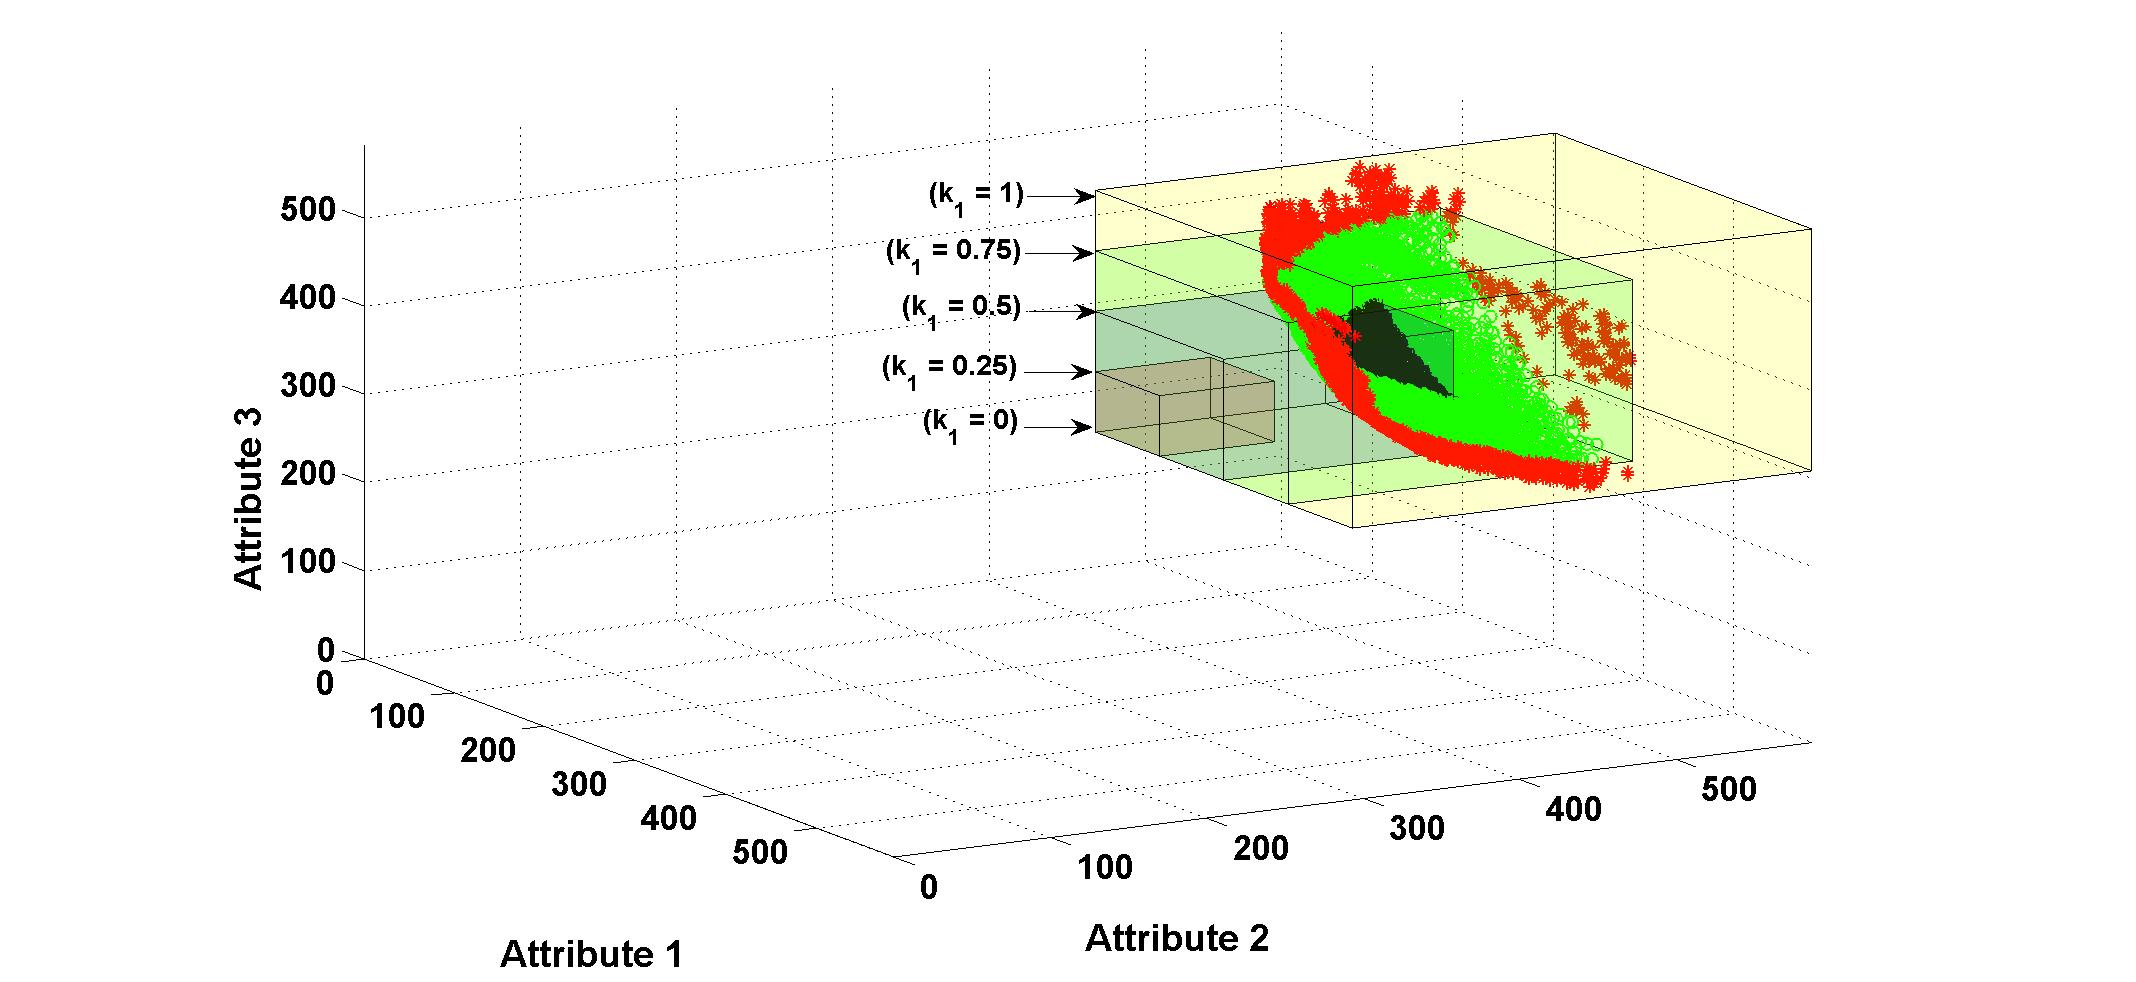
\includegraphics[width=1\textwidth]{Images/Chapter6/class1-3d-p45}
\caption{Three-dimensional Pareto frontier divided according to goal satisfiability for a sample problem with solution depth $d = 100$.}
\label{fig:6-1}
\end{figure}

Figures \ref{fig:6-2} and \ref{fig:6-3} display the average number of scanned labels and average runtimes of \lexgo and \namoa, respectively, both as a function of solution depth. In these graphics, we observe that \lexgolex \ (\ref{fig:6-3a}) achieves important reductions in time of almost one order of magnitude for $k_1=0.5$, two orders of magnitude for $k_1=0.25$, and up to four orders of magnitude for $k_1=0$. These are explained in large part by the reduction observed in the number of labels scanned, i.e. half the number of labels for $k_1=0.5$, around one order of magnitude less for $k_1=0.25$ and three orders of magnitude less for $k_1=0$. 

\begin{figure}%[!ht]
\centering
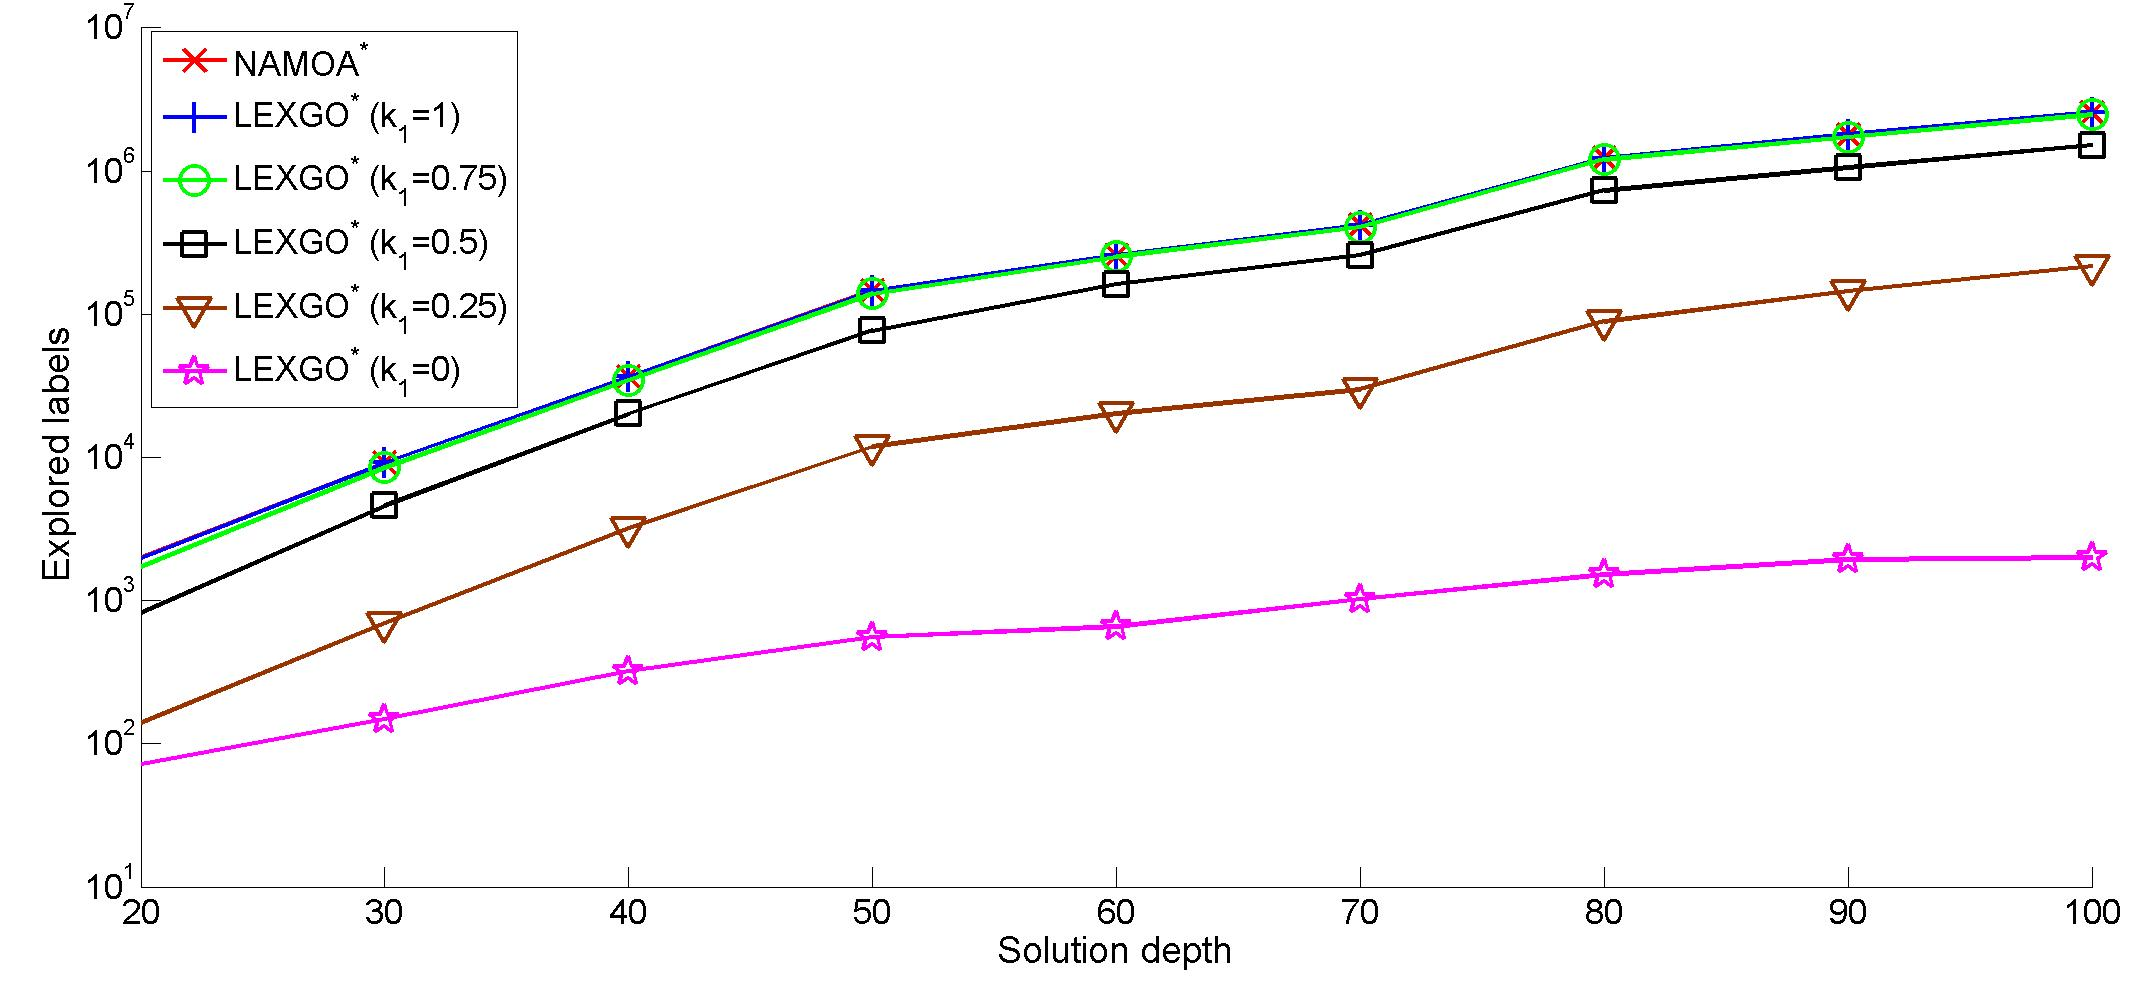
\includegraphics[width=1\textwidth]{Images/Chapter6/class1-labels-lex}
\caption{Class I experiments on grids, average number of scanned (explored) labels per solution depth for lexicographic selection order.}
\label{fig:6-2}
\end{figure}

Figure \ref{fig:6-3b} shows the average runtimes of \lexgolin \ and \namoalin. A small time overhead is also found for $k_1=0.75$ in the linear case, as well as poorer results when $k_1=0.5$. Notice that \namoalin \ is shown to be approximately two times faster than \namoalex. These results regarding the importance of the selection order are consistent with other recent studies \citep{Machuca2011, Iori2010}. However, \lexgolin \ is not always more efficient than \lexgolex. For $k_1= 1$ and $k_1= 0.75$ the linear aggregation order guides the search to find the solutions later than the lexicographic order and speeds up the runtime performance of algorithms that use the linear order whenever a big amount of solutions exist, due to a smaller number of filtering comparisons are needed. We further analyze in Section \ref{chapEmpiricalAnalysis:sec:resultsgridsnamoate} the impact of the number of pruning and filtering comparisons in runtime performance.

\begin{figure}
    \begin{center}
%
      \subfigure[Lexicographic selection order]{%
         \label{fig:6-3a}
        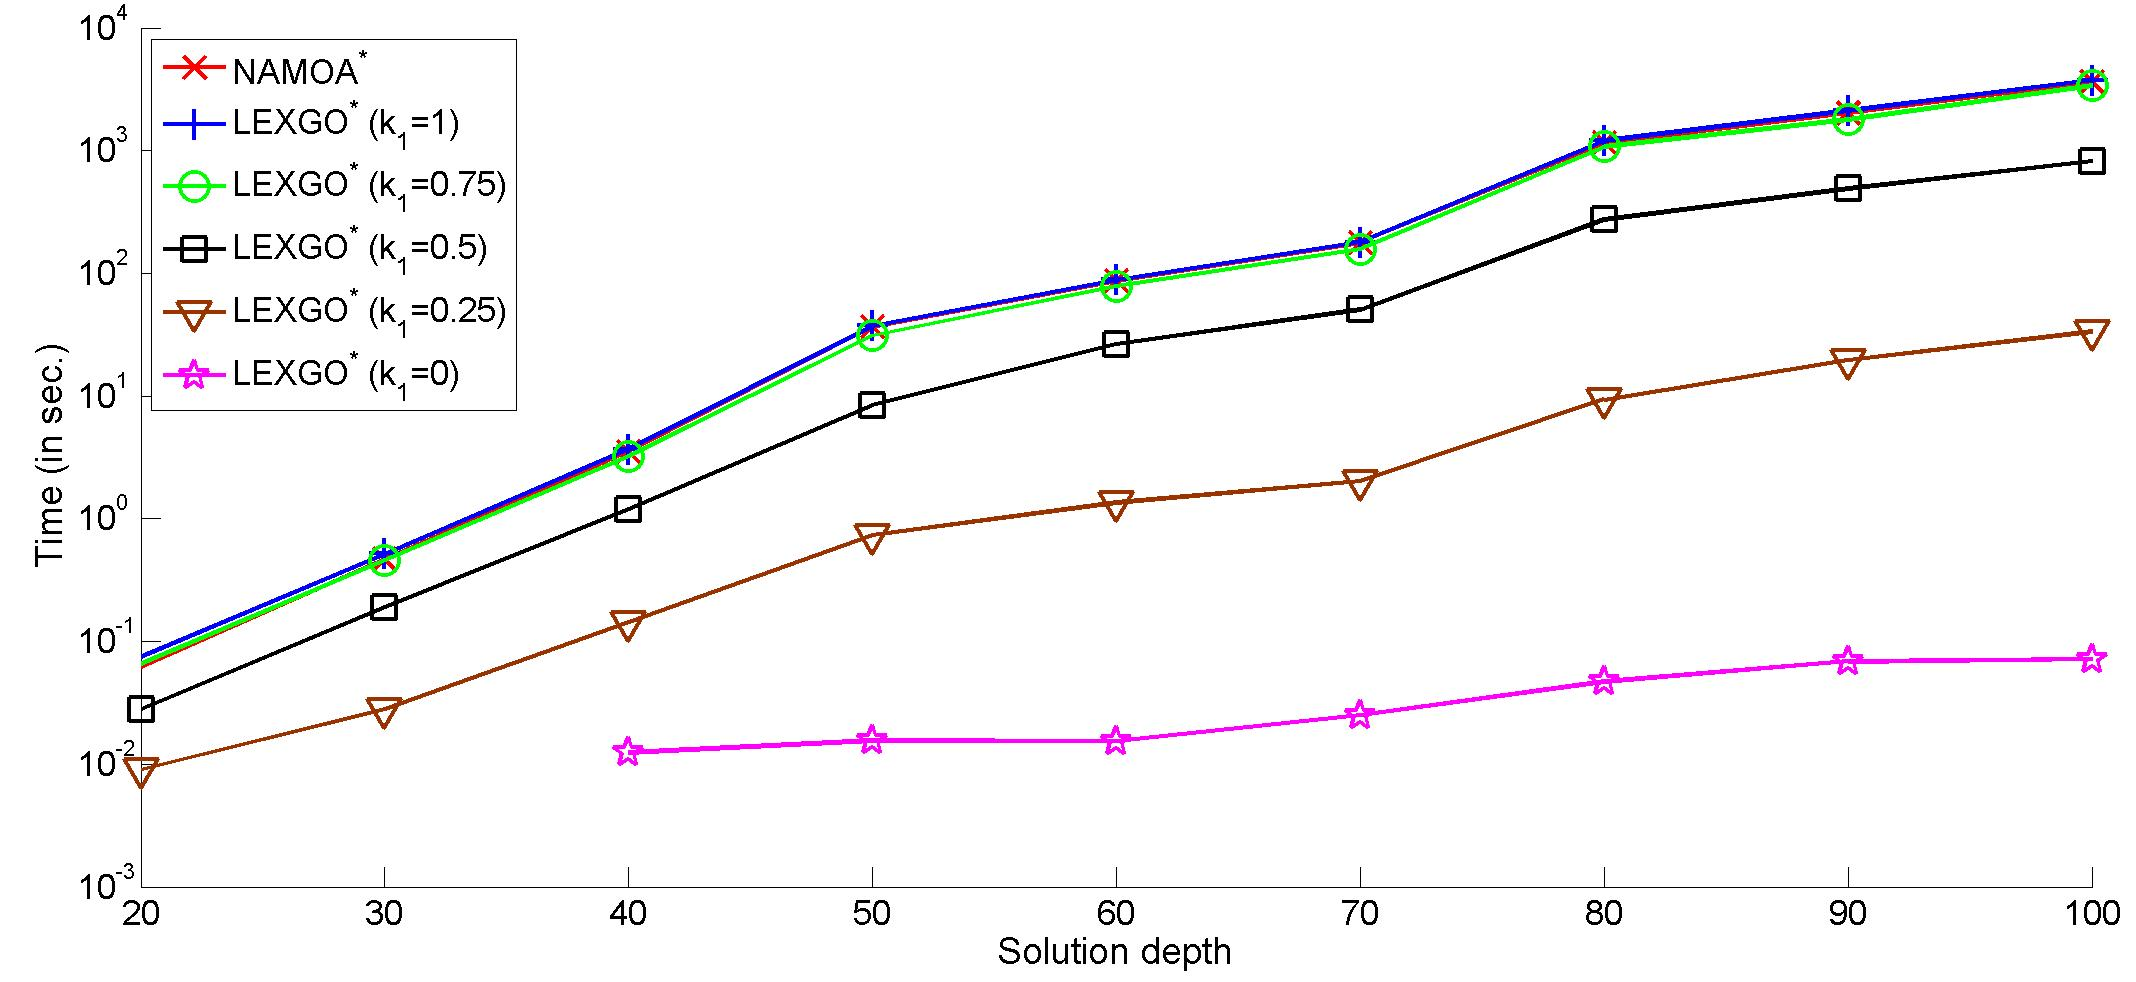
\includegraphics[width=0.95\textwidth]{Images/Chapter6/class1-exe-time-lex}
        }\\ %  ------- End of the first row ----------------------%
\vspace{0.025\textwidth}      
\subfigure[linear aggregation selection order]{%
         \label{fig:6-3b}
        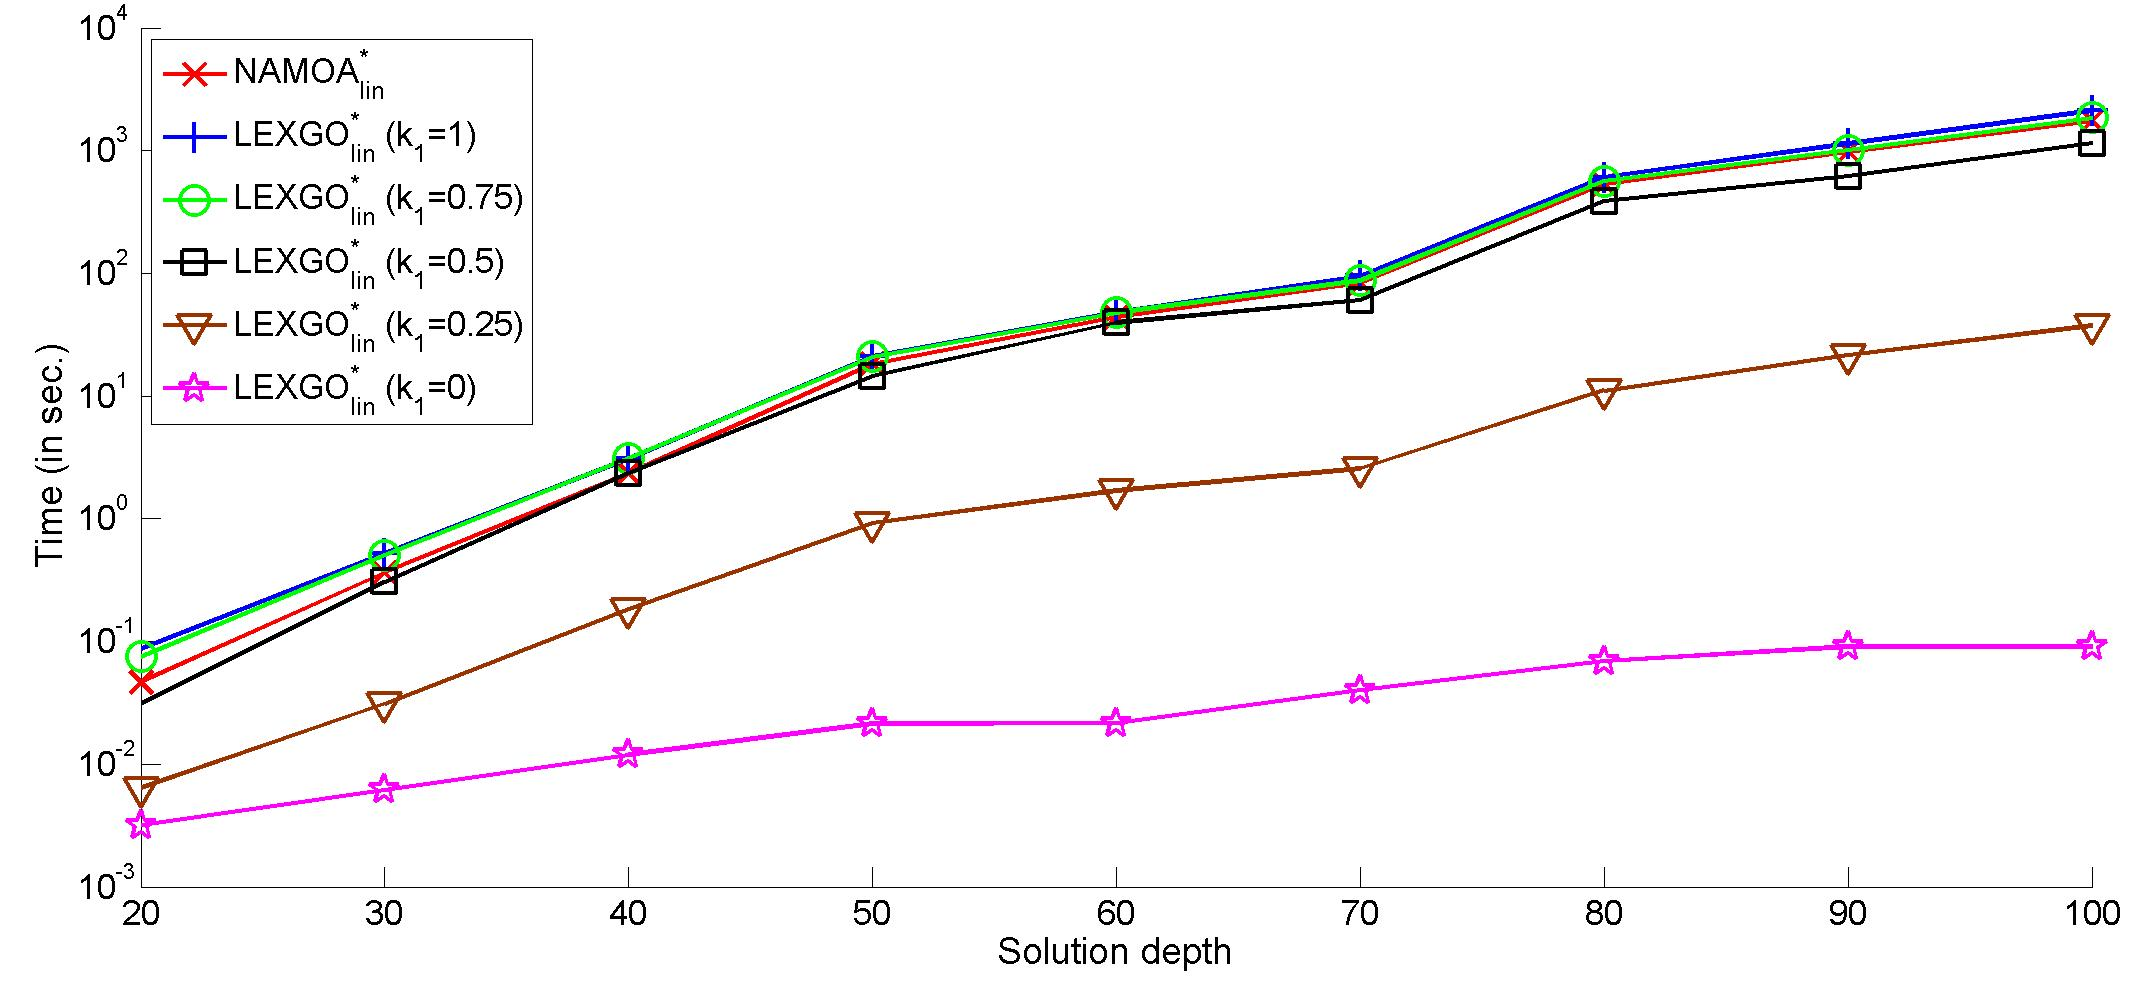
\includegraphics[width=0.95\textwidth]{Images/Chapter6/class1-exe-time-lin}
        }\\ %  ------- End of the first row ----------------------%
    \end{center}
    \vspace{-0.25in} 
    \caption{%
Class I experiments on grids, average runtime in seconds per solution depth for \namoa \ and \lexgo.  
    }%
    \label{fig:6-3}
\end{figure}

Table \ref{tab:6-2} summarizes the space and runtime performance of \lexgo \ relative to \namoa \ for $d = 100$ with the lexicographic and linear aggregation selection orders, respectively. The space performance is measured in scanned labels ($\sum G_{cl}$) and the runtime performance in seconds. 

A small time overhead can be observed for \lexgolex \ with $k_1= 1$ when compared with \namoalex. This time overhead is greater for \lexgolin, due to the comparison with the more efficient version of \namoa \ with the linear aggregation order. The time difference can be attributed to the extra calculations of deviation from targets needed by \lexgo \ for all labels, and the extra checks for pruning and filtering that do not provide any advantage in this situation.

No significant difference is found regarding the scanned labels by \namoalex \ and \namoalin, or the relative number to \lexgolex \ and \lexgolin. In fact, \namoa \ should expand the same labels regardless of the selection order policy. However, the lazy filtering technique introduces a slight variation which is found not to be significant in any case (see \cite{SandersMandow2013} for a more detailed explanation of the lazy filtering technique). 

\begin{table}
\caption{%
    Class I experiments on grids, summary of the relative space and runtime performance of \lexgo \ over \namoa \ for $d = 100$ experiments.
     }%
\vspace{0.05\textwidth}
\begin{center}
        \subtable[Relative space performance of \lexgolex \ over \namoalex]{%
\label{tab:6-2a}
\begin{tabular}{rrrrrrr}
\hline \noalign{\smallskip}
& \multicolumn{5}{c}{\lexgolex} \\
\noalign{\smallskip} \cline{2-6} \noalign{\smallskip}
\namoalex & 1 & 0.75 & 0.5 & 0.25 & 0 & \multicolumn{1}{c}{$k_1$} \\
\noalign{\smallskip} 
$\sum G_{cl}$ & \% & \% & \% & \% & \% \\
\cline{1-6}  \noalign{\smallskip} 
2,550,354 & 99.9 & 96.9 & 59.2 & 8.5 & 0.08 \\
\hline
\end{tabular}
        }%
\vspace{0.05\textwidth} % To get a little bit of space between the figures
        \subtable[Relative space performance of \lexgolin \ over \namoalin]{%
\label{tab:6-2b}
\begin{tabular}{rrrrrrr}
\hline \noalign{\smallskip}
& \multicolumn{5}{c}{\lexgolin} \\
\noalign{\smallskip} \cline{2-6} \noalign{\smallskip}
\namoalin & 1 & 0.75 & 0.5 & 0.25 & 0 & \multicolumn{1}{c}{$k_1$} \\
\noalign{\smallskip} 
$\sum G_{cl}$ & \% & \% & \% & \% & \% \\
\cline{1-6}  \noalign{\smallskip}  
2,598,427 & 99.9 & 97.2 & 59.1 & 8.3 & 0.08 \\
\hline
\end{tabular}
        }\\ %  ------- End of the first row ----------------------%
\vspace{0.05\textwidth}
        \subtable[Relative runtime performance of \lexgolex \ over \namoalex]{%
\label{tab:6-2c}
\begin{tabular}{rrrrrrr}
\hline \noalign{\smallskip}
& \multicolumn{5}{c}{\lexgolex} \\
\noalign{\smallskip} \cline{2-6} \noalign{\smallskip}
\namoalex & 1 & 0.75 & 0.5 & 0.25 & 0 & \multicolumn{1}{c}{$k_1$} \\
\noalign{\smallskip} 
Runtime (s) & \% & \% & \% & \% & \% \\
\cline{1-6}  \noalign{\smallskip} 
3,662.9 & 102.7 & 92.3 & 22.3 & 0.9 & 0.001 \\
\hline
\end{tabular}
        }%  %  ------- End of the second row ----------------------%
\vspace{0.05\textwidth}
        \subtable[Relative runtime performance of \lexgolin \ over \namoalin]{%
\label{tab:6-2d}
\begin{tabular}{rrrrrrr}
\hline \noalign{\smallskip}
& \multicolumn{5}{c}{\lexgolin} \\
\noalign{\smallskip} \cline{2-6} \noalign{\smallskip}
\namoalin & 1 & 0.75 & 0.5 & 0.25 & 0 & \multicolumn{1}{c}{$k_1$} \\
\noalign{\smallskip} 
Runtime (s) & \% & \% & \% & \% & \% \\
\cline{1-6}  \noalign{\smallskip} 
1,754.4 & 120.5 & 105.3 & 65.2 & 2.1 & 0.005 \\
\hline
\end{tabular}
        }%  %  ------- End of the third row ----------------------%
\end{center}
\label{tab:6-2}
\end{table}

%-------------------------------------------------------------------
\subsection{Analysis on class II experiments}
\label{chapEmpiricalAnalysis:subsec:analysisgridslexgoc2}
%-------------------------------------------------------------------

Target values in the second class of experiments were defined using $k_1 = \{0.75 , 0.5\}$, where $k_2$ is defined as in Equation \ref{eq:targets2}. This allows us to analyze the case where targets for one goal are proportionally stricter, and the extreme case where some goals are satisfied and some not. 

Tables \ref{tab:6-3} and \ref{tab:6-4} show percentages of Pareto goal-optimal solution costs and scanned labels of all values of $k_2$ in \lexgo \ relative to \namoa. Figure \ref{fig:6-4} displays the average number of scanned labels as a function of solution depth for $k_1= 0.75$ and $k_1= 0.5$.

\begin{table}
\caption{Class II experiments on grids, \lexgo \ average percentage of goal-optimal solution costs relative to $C^*$. An asterisk ($^*$) indicates some of the five instances could not satisfy all goals, and two asterisks ($^{**}$) that none of the five instances could satisfy all goals.}
\centering
\begin{tabular}{rrrrrrrrrrr}
\hline \noalign{\smallskip}
 & & \multicolumn{8}{c}{\lexgo} & \\
\noalign{\smallskip} \cline{3-10}
\multicolumn{2}{c}{} & \multicolumn{4}{c|}{0.75} & \multicolumn{4}{c}{0.5} & \multicolumn{1}{c}{$k_1$}\\
 & \namoa & 0.75 & 0.5625 & 0.375 & \multicolumn{1}{c|}{0.1875} & 0.5 & 0.375 & 0.25 & 0.125 & \multicolumn{1}{c}{$k_2$}\\
\noalign{\smallskip} 
$d$ & Avg. $|C^*|$ & \% & \% & \% & \% & \% & \% & \% & \% & \\
\cline{1-10} \noalign{\smallskip} 
20 & 122 & 74.3 & 59.1 & 35.2 & 10.6 & 20.5 & 11.5 & 3.3 & $^*$0.82 \\ 
30 & 302 & 77.6 & 63.4 & 38.5 & 15.5 & 22.2 & 12.3 & 5.6 & $^*$1.00 \\
40 & 694 & 78.7 & 59.3 & 34.0 & 12.2 & 20.8 & 10.5 & 3.3 & $^{**}$0.14 \\
50 & 1,599 & 78.2 & 57.2 & 33.6 & 12.3 & 16.8 & 8.4 & 2.6 & $^*$0.06 \\
60 & 2,007 & 83.0 & 62.6 & 35.9 & 12.6 & 24.6 & 13.1 & 3.8 & $^*$0.25 \\ 
70 & 2,561 & 82.4 & 66.0 & 41.9 & 14.6 & 24.6 & 13.6 & 4.2 & $^*$0.12 \\ 
80 & 5,423 & 82.3 & 64.9 & 36.1 & 11.6 & 20.3 & 9.1 & 1.7 & $^{**}$0.02 \\ 
90 & 5,912 & 77.7 & 63.6 & 38.2 & 10.7 & 21.0 & 10.5 & 2.1 & $^{**}$0.02 \\ 
100 & 8,307 & 77.9 & 60.5 & 35.7 & 10.6 & 17.0 & 8.1 & 1.1 & $^{**}$0.01 
\\ 
\hline
\end{tabular}
\label{tab:6-3}
\end{table} 

\begin{table}
\caption{Class II experiments on grids, \lexgolex \ average percentage of scanned labels ($\sum G_{cl}$) compared to \namoalex.}
\centering
\begin{tabular}{rrrrrrrrrrr}
\hline \noalign{\smallskip}
 & & \multicolumn{8}{c}{\lexgolex} & \\
\noalign{\smallskip} \cline{3-10}
\multicolumn{2}{c}{} & \multicolumn{4}{c|}{0.75} & \multicolumn{4}{c}{0.5} & \multicolumn{1}{c}{$k_1$}\\
 & \namoalex & 0.75 & 0.5625 & 0.375 & \multicolumn{1}{c|}{0.1875} & 0.5 & 0.375 & 0.25 & 0.125 & \multicolumn{1}{c}{$k_2$}\\
\noalign{\smallskip} 
$d$ & $\sum G_{cl}$  & \% & \% & \% & \% & \% & \% & \% & \% & \\
\cline{1-10} \noalign{\smallskip} 
20 & 1,985 & 86.2 & 75.1 & 50.9 & 19.0 & 41.4 & 28.9 & 17.5 & 8.9 \\ 
30 & 9,164 & 92.4 & 83.1 & 55.5 & 20.3 & 50.3 & 34.8 & 18.9 & 11.0 \\
40 & 36,557 & 94.5 & 83.2 & 55.6 & 19.1 & 55.1 & 38.4 & 19.9 & 9.5 \\
50 & 145,823 & 95.5 & 83.4 & 54.7 & 18.3 & 52.7 & 36.4 & 18.2 & 7.5 \\
60 & 257,935 & 97.5 & 88.9 & 60.9 & 19.8 & 62.9 & 45.9 & 23.1 & 7.8 \\ 
70 & 420,056 & 96.6 & 88.9 & 63.5 & 21.2 & 61.5 & 45.7 & 23.5 & 7.2 \\ 
80 & 1,231,565 & 97.3 & 89.1 & 60.4 & 18.8 & 59.2 & 42.0 & 20.0 & 8.6 \\ 
90 & 1,789,607 & 96.7 & 88.8 & 62.9 & 20.0 & 59.1 & 43.1 & 21.6 & 10.3 \\ 
100 & 2,550,354 & 97.0 & 89.3 & 61.1 & 17.5 & 59.3 & 42.2 & 19.8 & 11.8 \\ 
\hline
\end{tabular}
\label{tab:6-4}
\end{table} 

\begin{figure}
    \begin{center}
%
      \subfigure[$k_1 = 0.75$]{%
         \label{fig:6-4a}
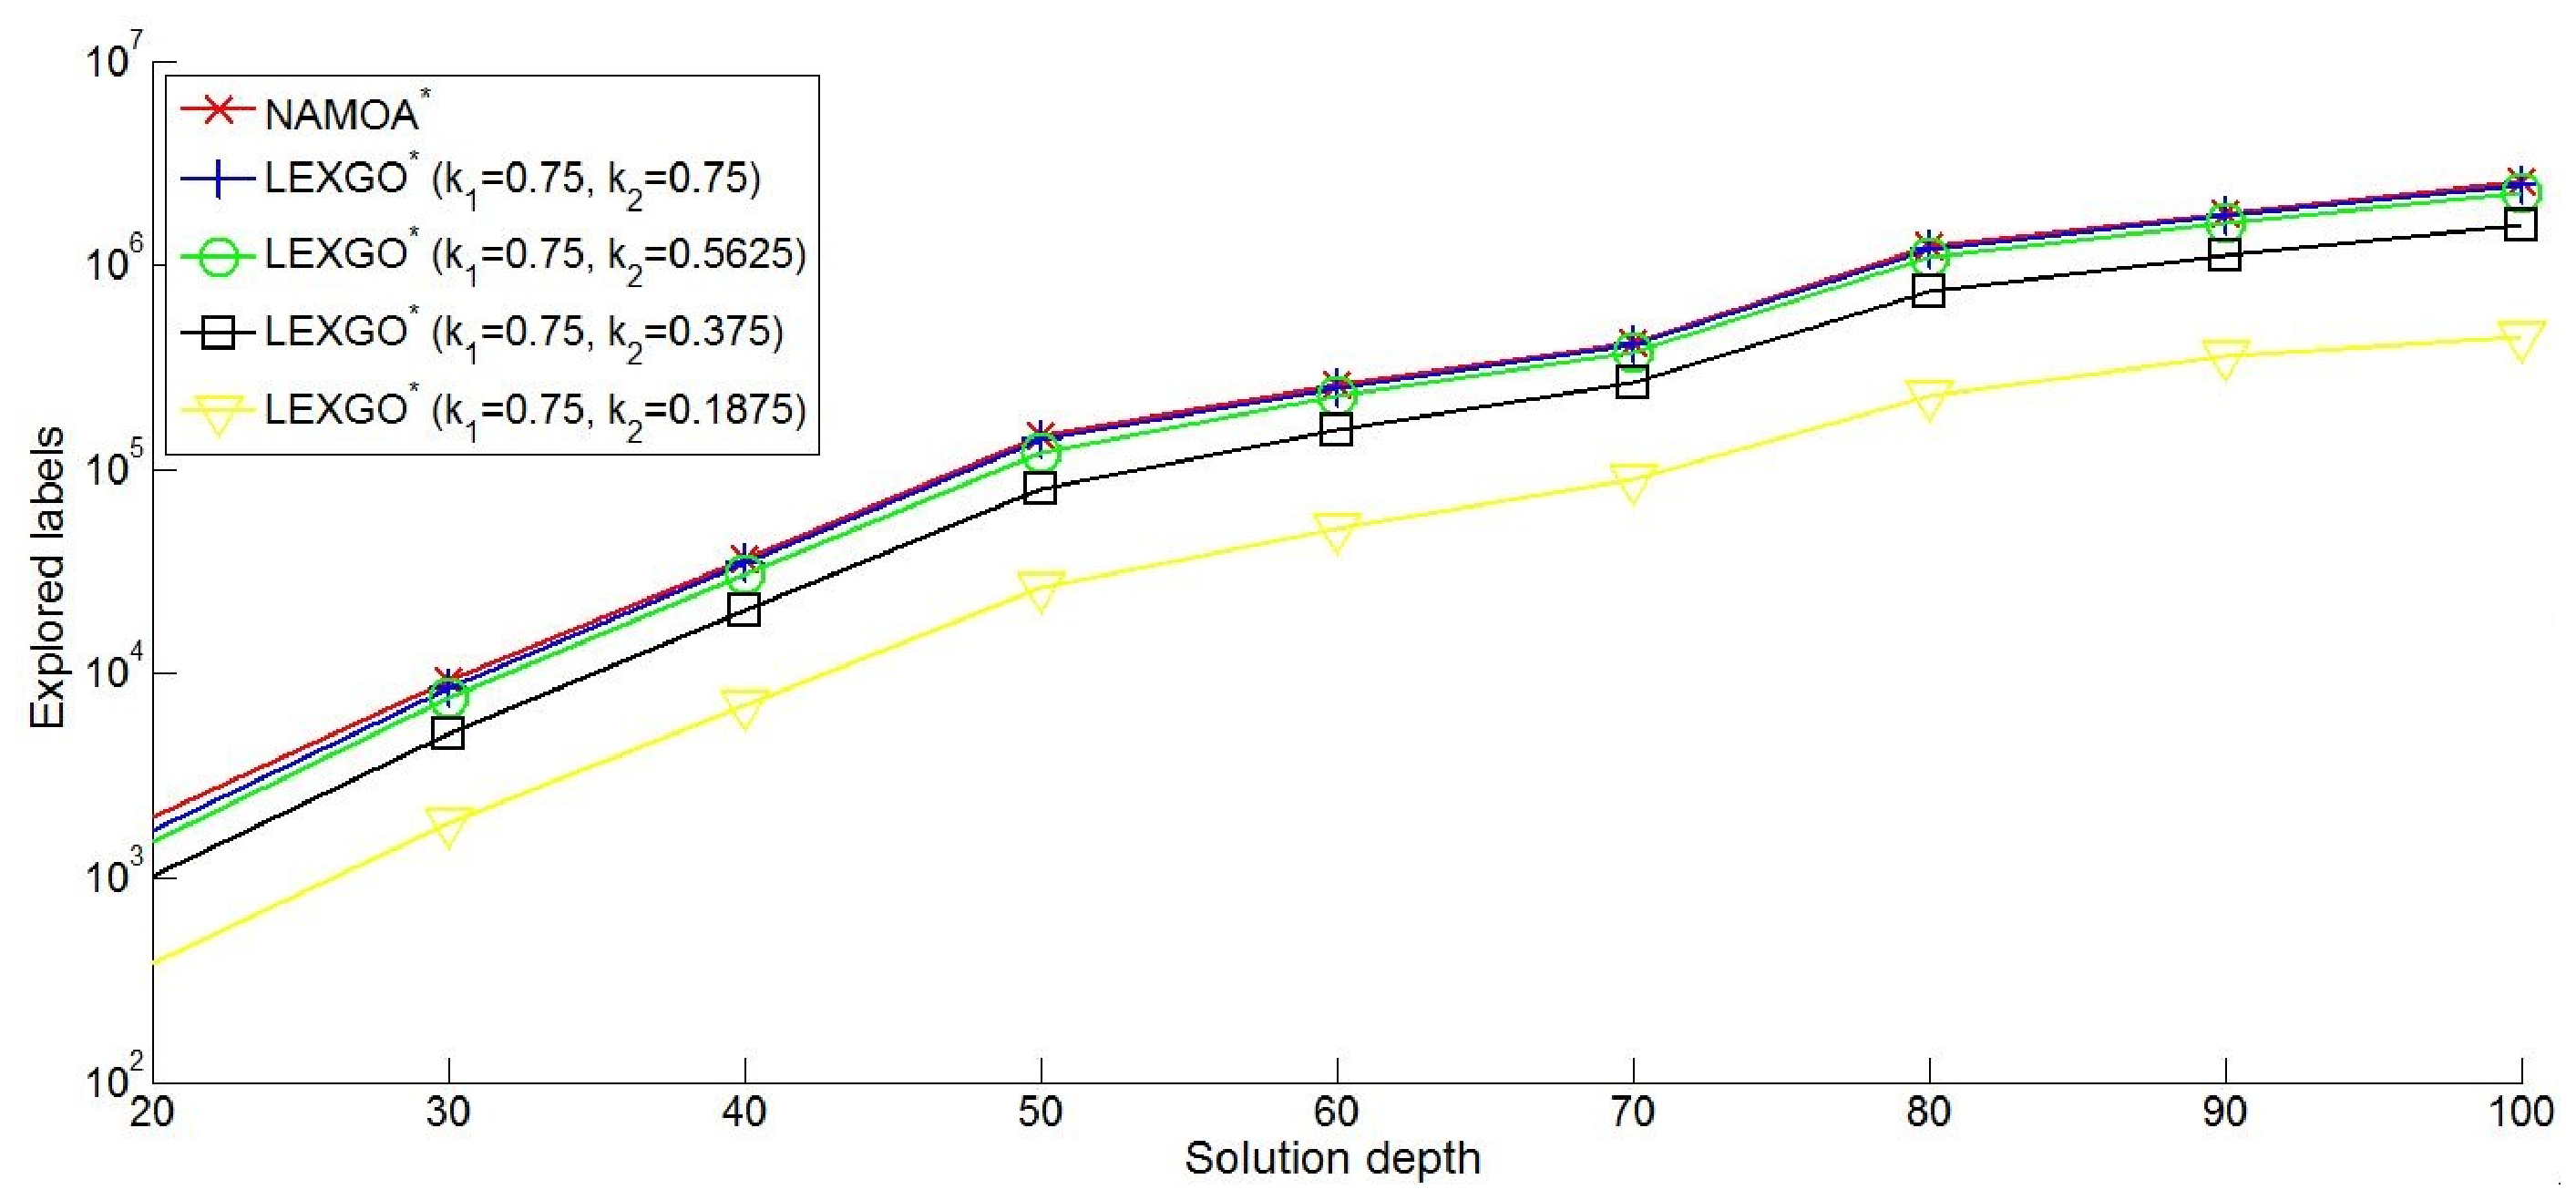
\includegraphics[width=0.95\textwidth]{Images/Chapter6/class2-labels075-lex}
        }\\ %  ------- End of the first row ----------------------%
\vspace{0.025\textwidth}      
		\subfigure[$k_1 = 0.5$]{%
         \label{fig:6-4b}  
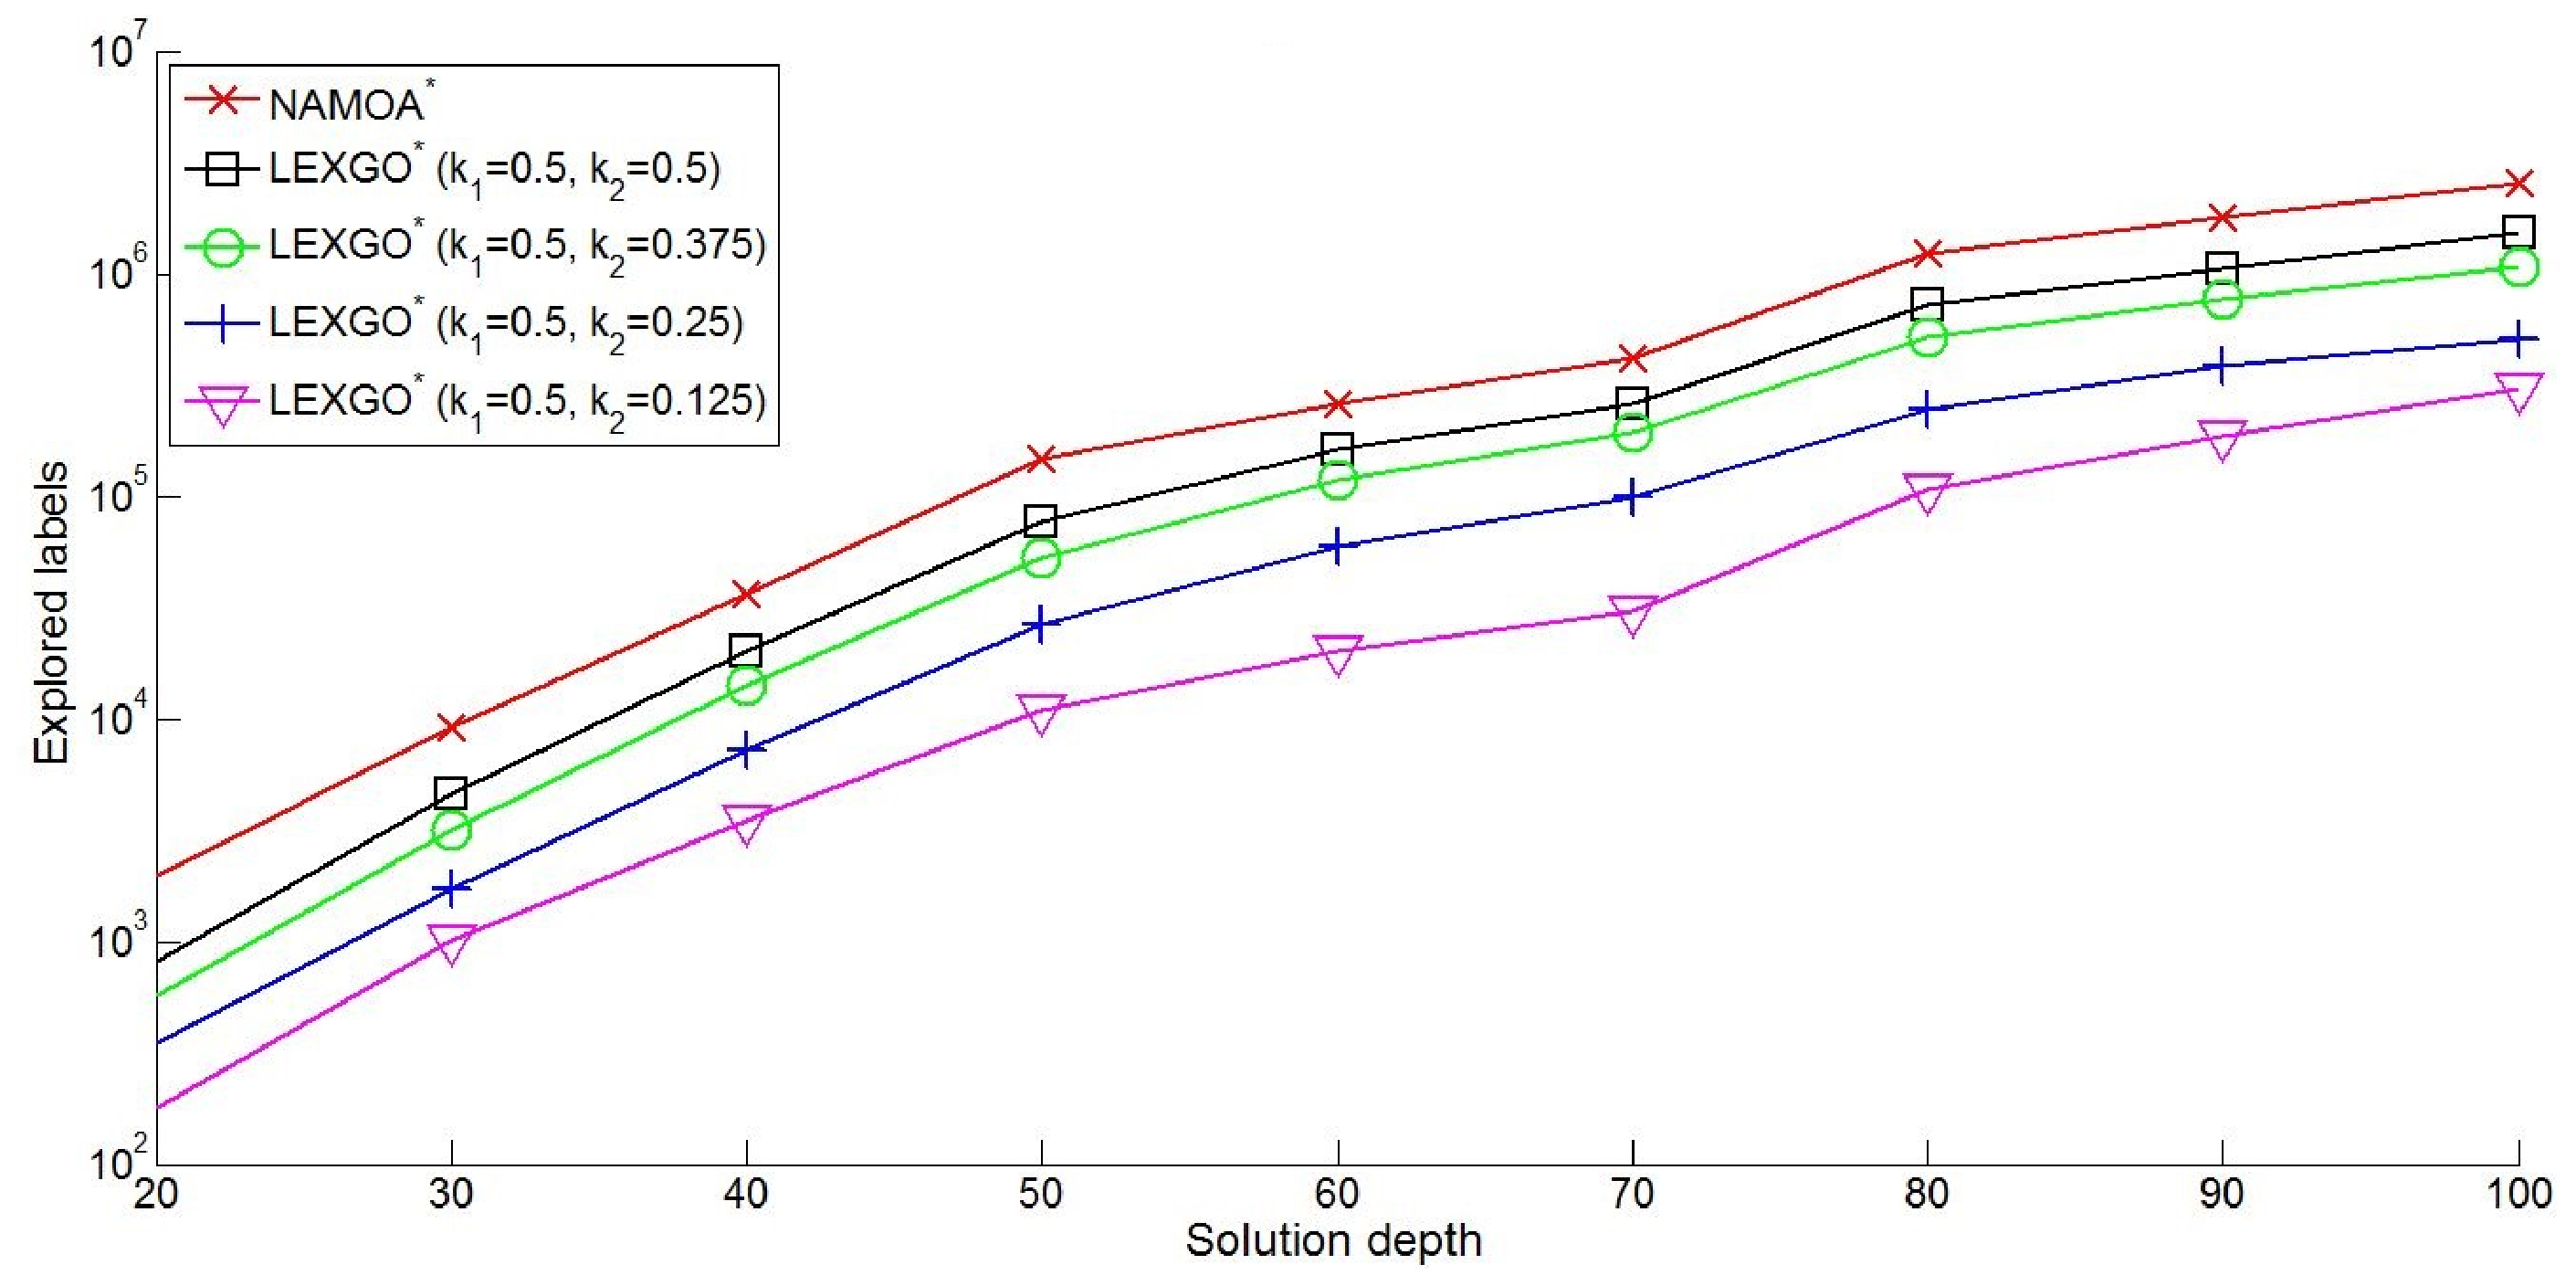
\includegraphics[width=0.95\textwidth]{Images/Chapter6/class2-labels05-lex}
        }\\ %  ------- End of the first row ----------------------%
    \end{center}
    \vspace{-0.25in} 
    \caption{%
Class II experiments on grids, average scanned labels per solution depth for \namoa \ and \lexgo \ with lexicographic selection order.  
    }%
    \label{fig:6-4}
\end{figure}

Table \ref{tab:6-5} displays the relative percentage of \lexgo \ runtimes to \namoa \ employing lexicographic and linear selection orders. In a graphical manner, Figures \ref{fig:6-5} and \ref{fig:6-6} show, respectively, average runtimes for  $k_1 = 0.75$ and $k_1 = 0.5$ with lexicographic and linear selection orders.

\begin{table}
\caption{%
Class II experiments on grids, \lexgo \ runtimes (in seconds) percentage relative to \namoa.
     }%
\begin{center}
        \subtable[Lexicographic selection order]{%
\label{tab:6-5a}
\scalebox{.95}{
\begin{tabular}{rrrrrrrrrrr}
\hline \noalign{\smallskip}
 & & \multicolumn{8}{c}{\lexgolex} & \\
\noalign{\smallskip} \cline{3-10}
\multicolumn{2}{c}{} & \multicolumn{4}{c|}{0.75} & \multicolumn{4}{c}{0.5} & \multicolumn{1}{c}{$k_1$}\\
 & \namoalex & 0.75 & 0.5625 & 0.375 & \multicolumn{1}{c|}{0.1875} & 0.5 & 0.375 & 0.25 & 0.125 & \multicolumn{1}{c}{$k_2$}\\
\noalign{\smallskip} 
$d$ & Runtime (s) & \% & \% & \% & \% & \% & \% & \% & \% & \\
\cline{1-10} \noalign{\smallskip} 
20 & 0.06 & 100.0 & 66.6 & 50.0 & 16.6 & 33.3 & 16.6 & 1.6 & 1.6 \\ 
30 & 0.4 & 112.5 & 95.0 & 55.0 & 17.5 & 47.5 & 30.0 & 17.5 & 12.5 \\ 
40 & 3.5 & 91.4 & 68.5 & 34.2 & 8.5 & 34.2 & 20.0 & 8.5 & 5.7 \\ 
50 & 36.8 & 84.7 & 60.0 & 25.8 & 4.6 & 22.8 & 12.5 & 4.8 & 1.9 \\ 
60 & 86.9 & 90.6 & 67.4 & 29.4 & 4.4 & 30.4 & 16.6 & 5.8 & 1.8 \\  
70 & 178.5 & 88.4 & 67.5 & 31.2 & 4.9 & 28.1 & 15.1 & 5.3 & 1.4 \\
80 & 1,164.1 & 92.2 & 69.5 & 27.8 & 3.4 & 23.5 & 11.6 & 3.4 & 1.4 \\ 
90 & 2,030.0 & 87.7 & 69.0 & 31.4 & 3.7 & 24.1 & 12.6 & 3.9 & 1.9 \\ 
100 & 3,662.9 & 92.3 & 66.7 & 27.6 & 2.9 & 22.3 & 11.1 & 3.3 & 2.1 \\ 
\hline
\end{tabular}
}
        }%
\vspace{0.05\textwidth} % To get a little bit of space between the figures
        \subtable[linear aggregation selection order]{%
\label{tab:6-5b}
\scalebox{.95}{
\begin{tabular}{rrrrrrrrrrr}
\hline \noalign{\smallskip}
 & & \multicolumn{8}{c}{\lexgolin} & \\
\noalign{\smallskip} \cline{3-10}
\multicolumn{2}{c}{} & \multicolumn{4}{c|}{0.75} & \multicolumn{4}{c}{0.5} & \multicolumn{1}{c}{$k_1$}\\
 & \namoalin & 0.75 & 0.5625 & 0.375 & \multicolumn{1}{c|}{0.1875} & 0.5 & 0.375 & 0.25 & 0.125 & \multicolumn{1}{c}{$k_2$}\\
\noalign{\smallskip} 
$d$ & Runtime (s) & \% & \% & \% & \% & \% & \% & \% & \% & \\
\cline{1-10} \noalign{\smallskip} 
20 & 0.04 & 160.3 & 146.6 & 100.4 & 40.2 & 66.2 & 46.6 & 32.9 & 19.7 \\ 
30 & 0.3 & 138.4 & 149.5 & 99.9 & 30.8 & 83.8 & 58.1 & 28.2 & 16.3 \\ 
40 & 2.3 & 131.3 & 174.6 & 104.2 & 25.4 & 99.7 & 62.7 & 26.3 & 11.5 \\ 
50 & 18.3 & 113.6 & 144.0 & 92.5 & 17.6 & 79.2 & 50.4 & 18.1 & 5.3 \\ 
60 & 43.8 & 108.8 & 138.6 & 95.8 & 16.1 & 90.2 & 61.9 & 22.6 & 4.8 \\  
70 & 83.3 & 104.4 & 117.4 & 101.3 & 19.5 & 72.6 & 56.9 & 21.2 & 4.2 \\
80 & 533.8 & 105.5 & 138.3 & 96.4 & 13.8 & 72.6 & 49.6 & 14.6 & 4.0 \\ 
90 & 981.3 & 102.6 & 121.4 & 92.4 & 12.8 & 63.3 & 48.2 & 15.5 & 4.8 \\ 
100 & 1,754.4 & 105.3 & 130.2 & 98.0 & 11.1 & 65.3 & 46.1 & 13.1 & 5.3 \\ 
\hline
\end{tabular}
}
        }\\ %  ------- End of the first row ----------------------%
\end{center}
\label{tab:6-5}
\end{table}

\begin{figure}
    \begin{center}
%
      \subfigure[$k_1 = 0.75$]{%
         \label{fig:6-5a}
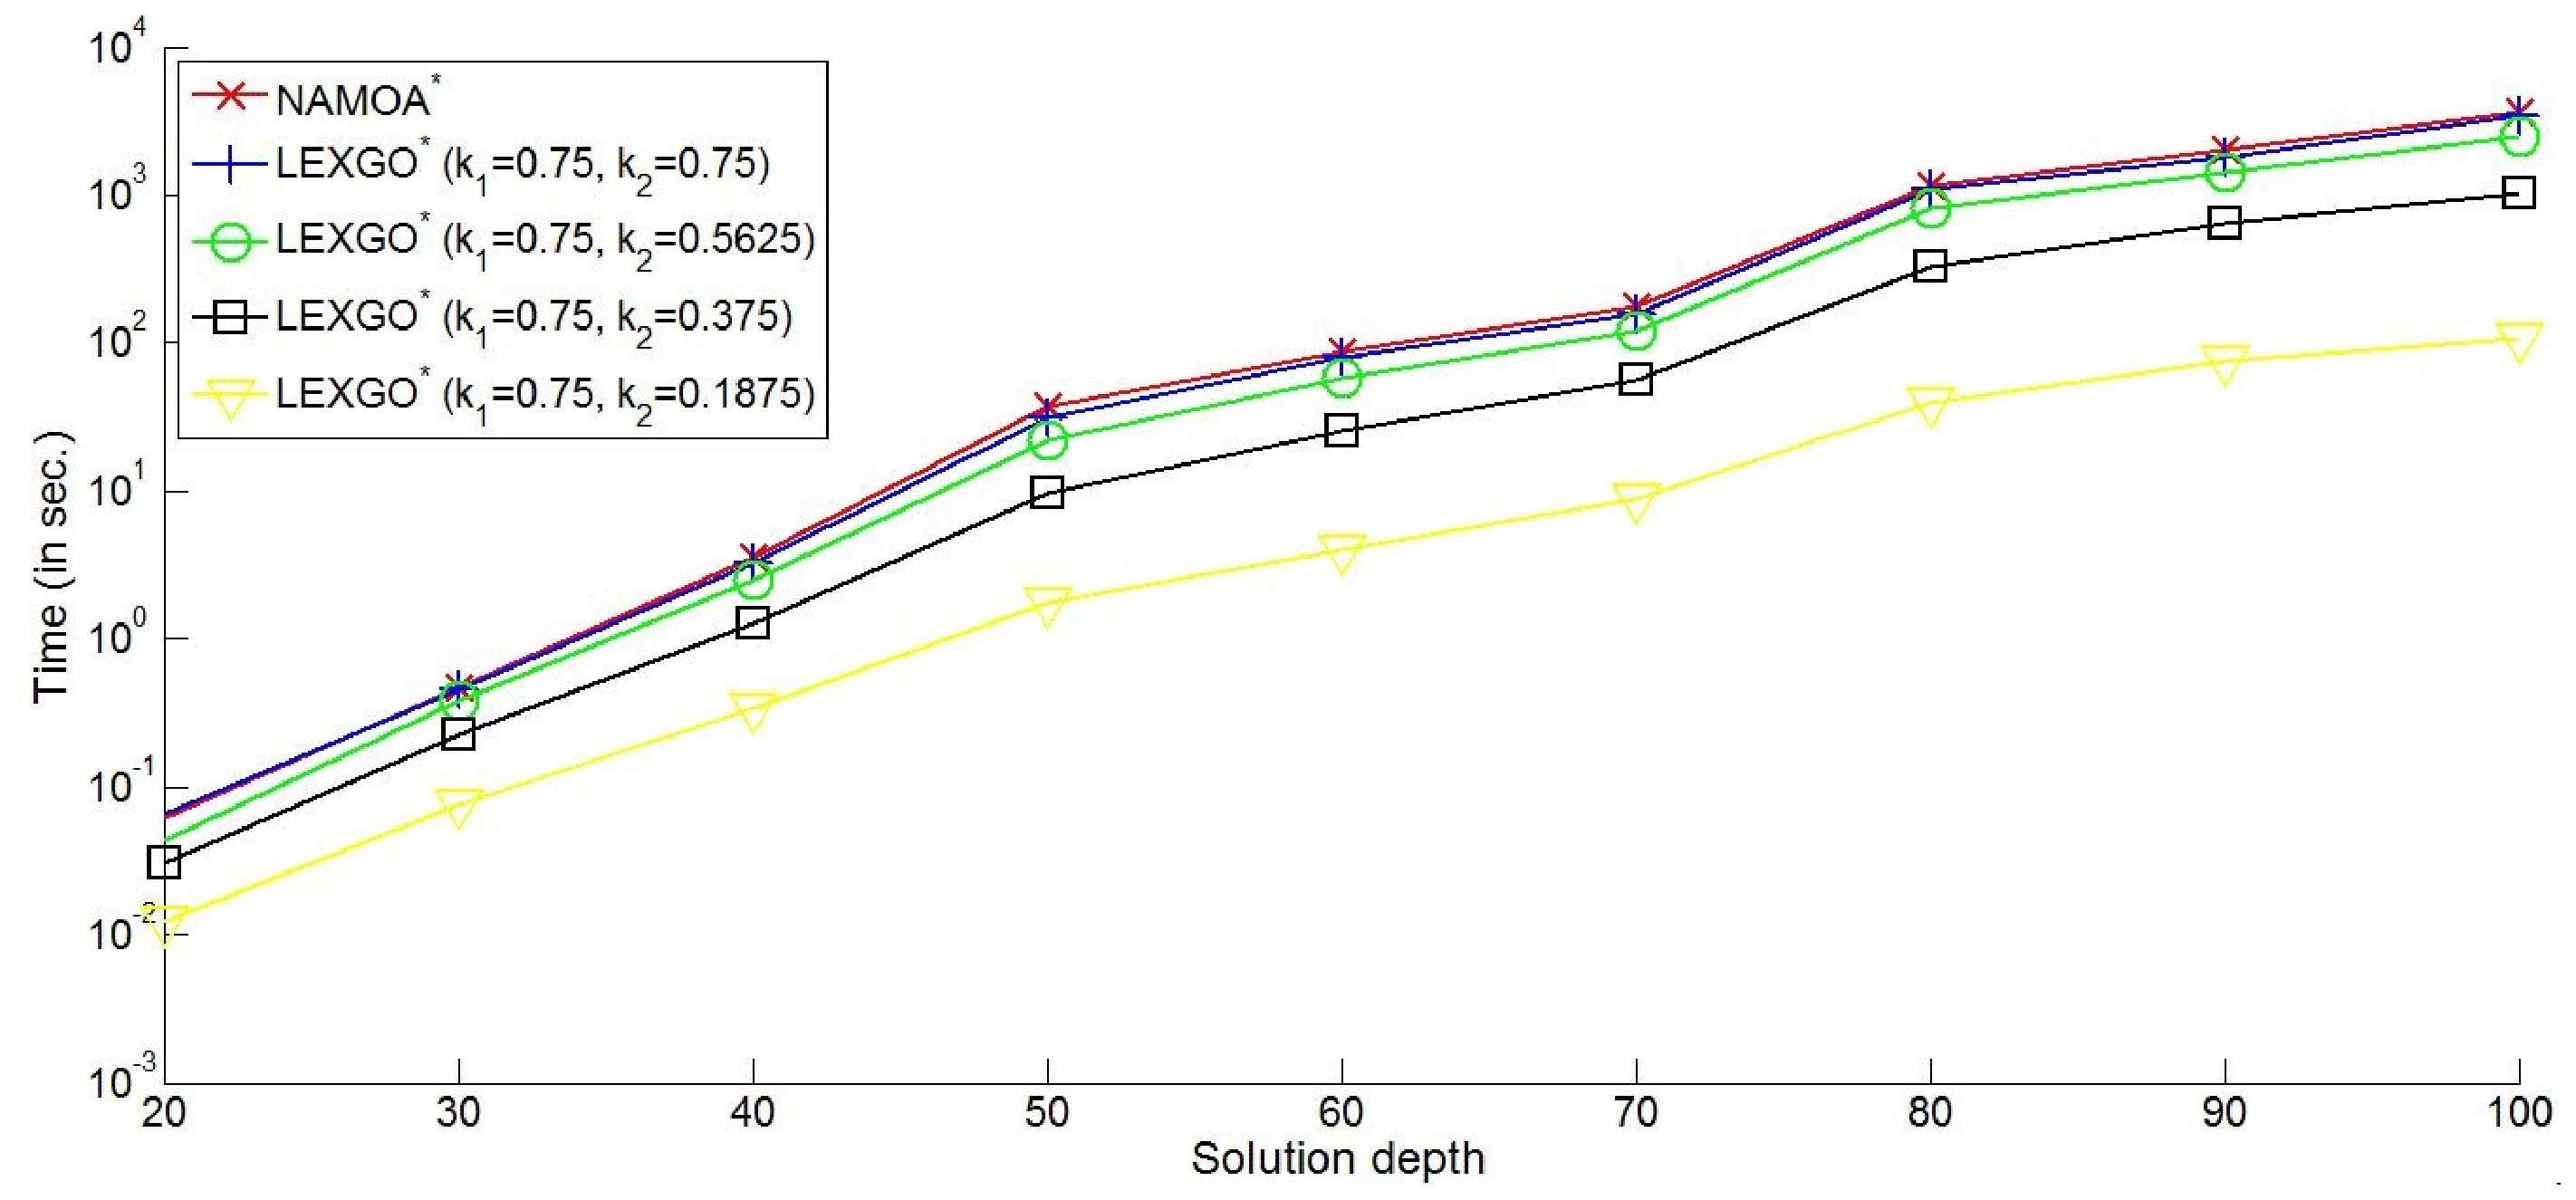
\includegraphics[width=0.95\textwidth]{Images/Chapter6/class2-exe075-lex}
        }\\ %  ------- End of the first row ----------------------%
\vspace{0.025\textwidth}      
		\subfigure[$k_1 = 0.5$]{%
         \label{fig:6-5b}  
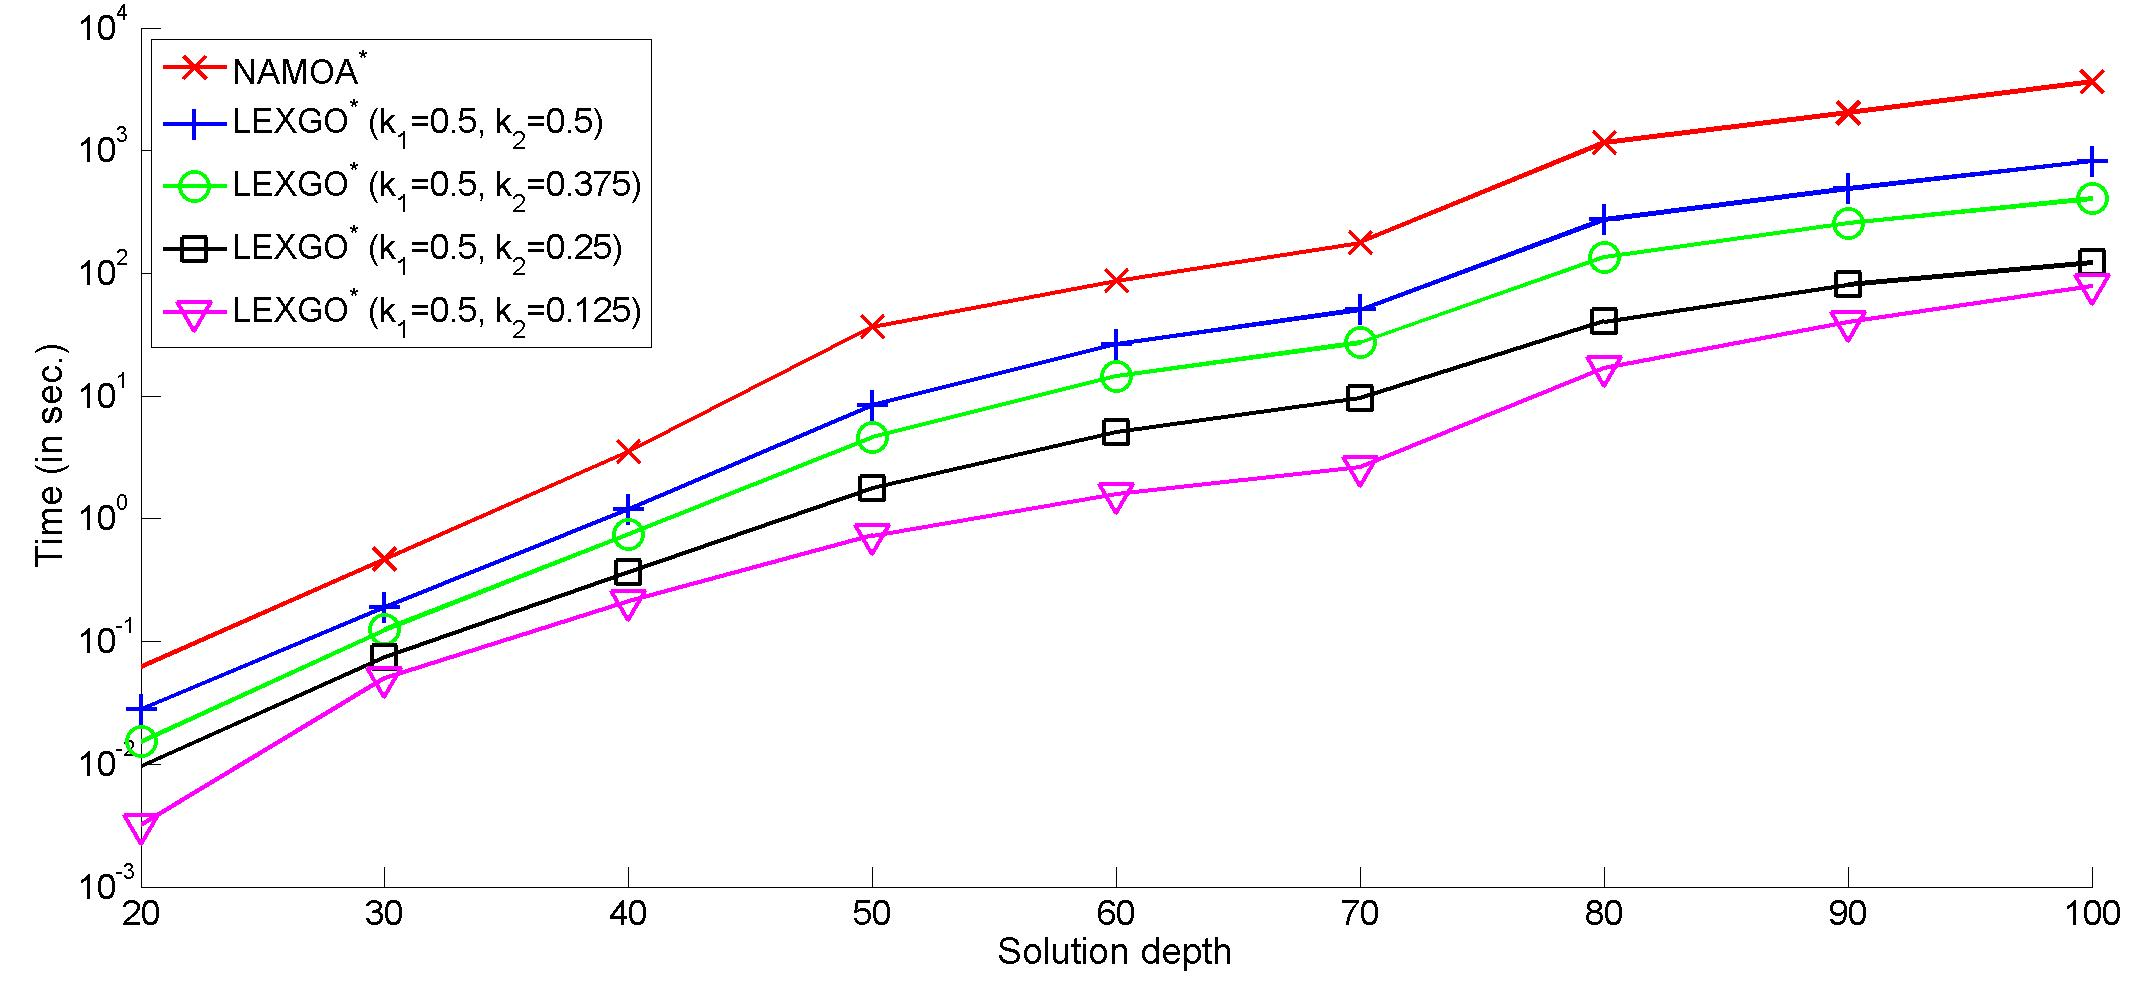
\includegraphics[width=0.95\textwidth]{Images/Chapter6/class2-exe05-lex}
        }\\ %  ------- End of the first row ----------------------%
    \end{center}
    \vspace{-0.25in} 
    \caption{%
Class II experiments on grids, average runtime (in seconds) per solution depth for \lexgo \ and \namoa \ with lexicographic selection order. 
    }%
    \label{fig:6-5}
\end{figure}

\begin{figure}
    \begin{center}
%
      \subfigure[$k_1 = 0.75$]{%
         \label{fig:6-6a}
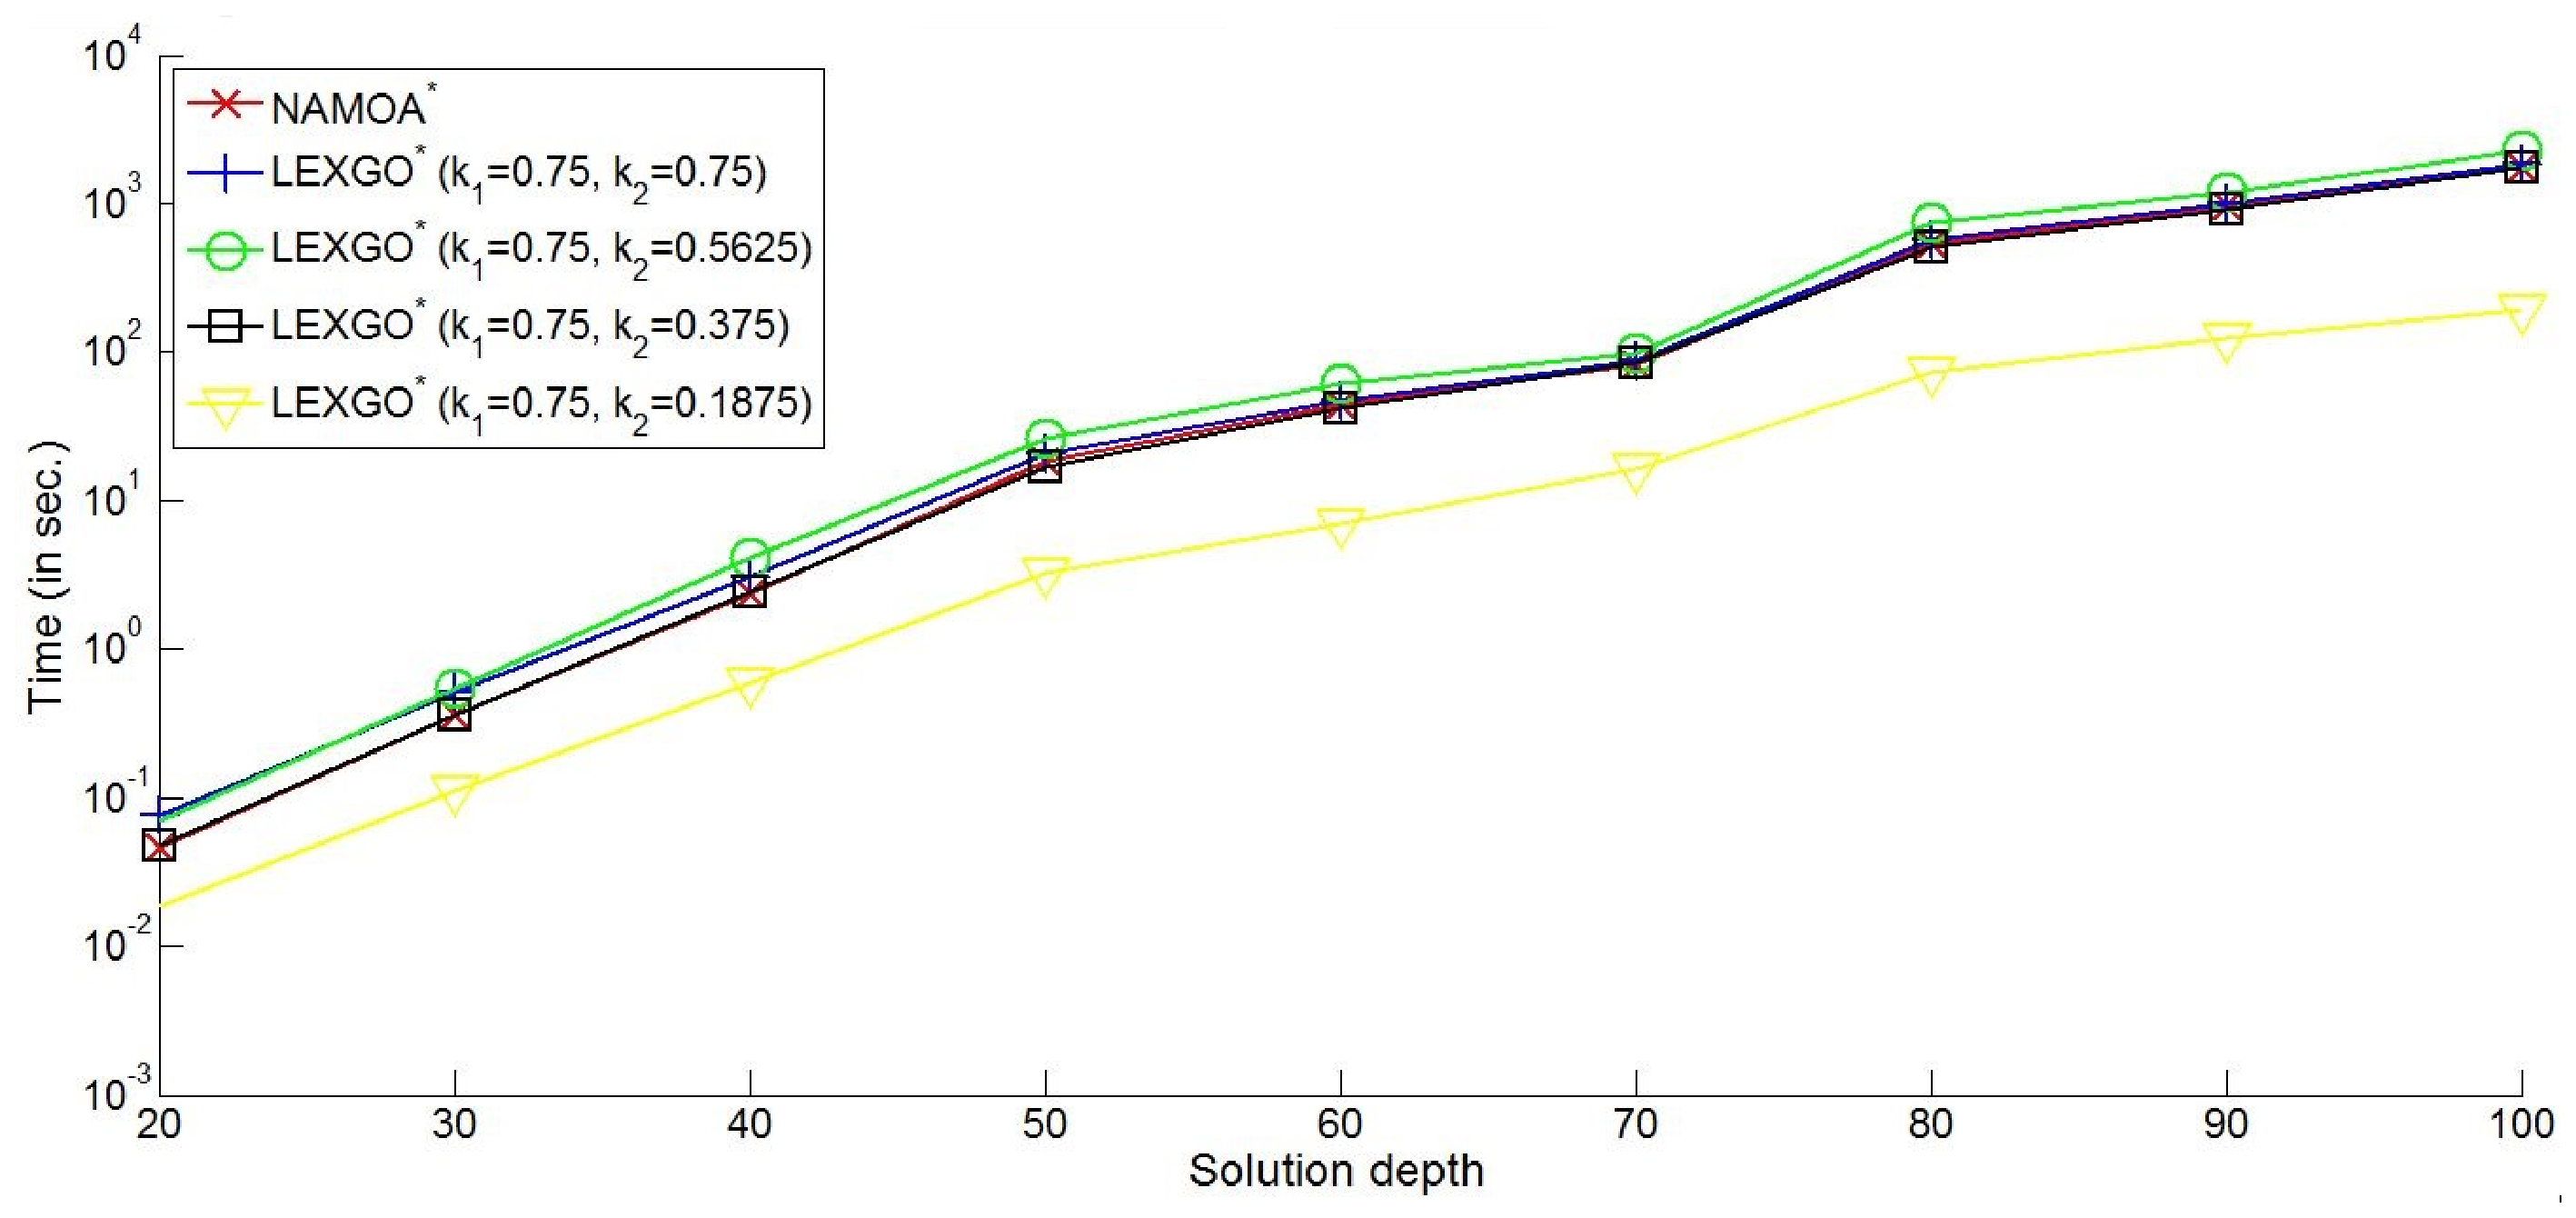
\includegraphics[width=0.95\textwidth]{Images/Chapter6/class2-exe075-lin}
        }\\ %  ------- End of the first row ----------------------%
\vspace{0.025\textwidth}      
		\subfigure[$k_1 = 0.5$]{%
         \label{fig:6-6b}  
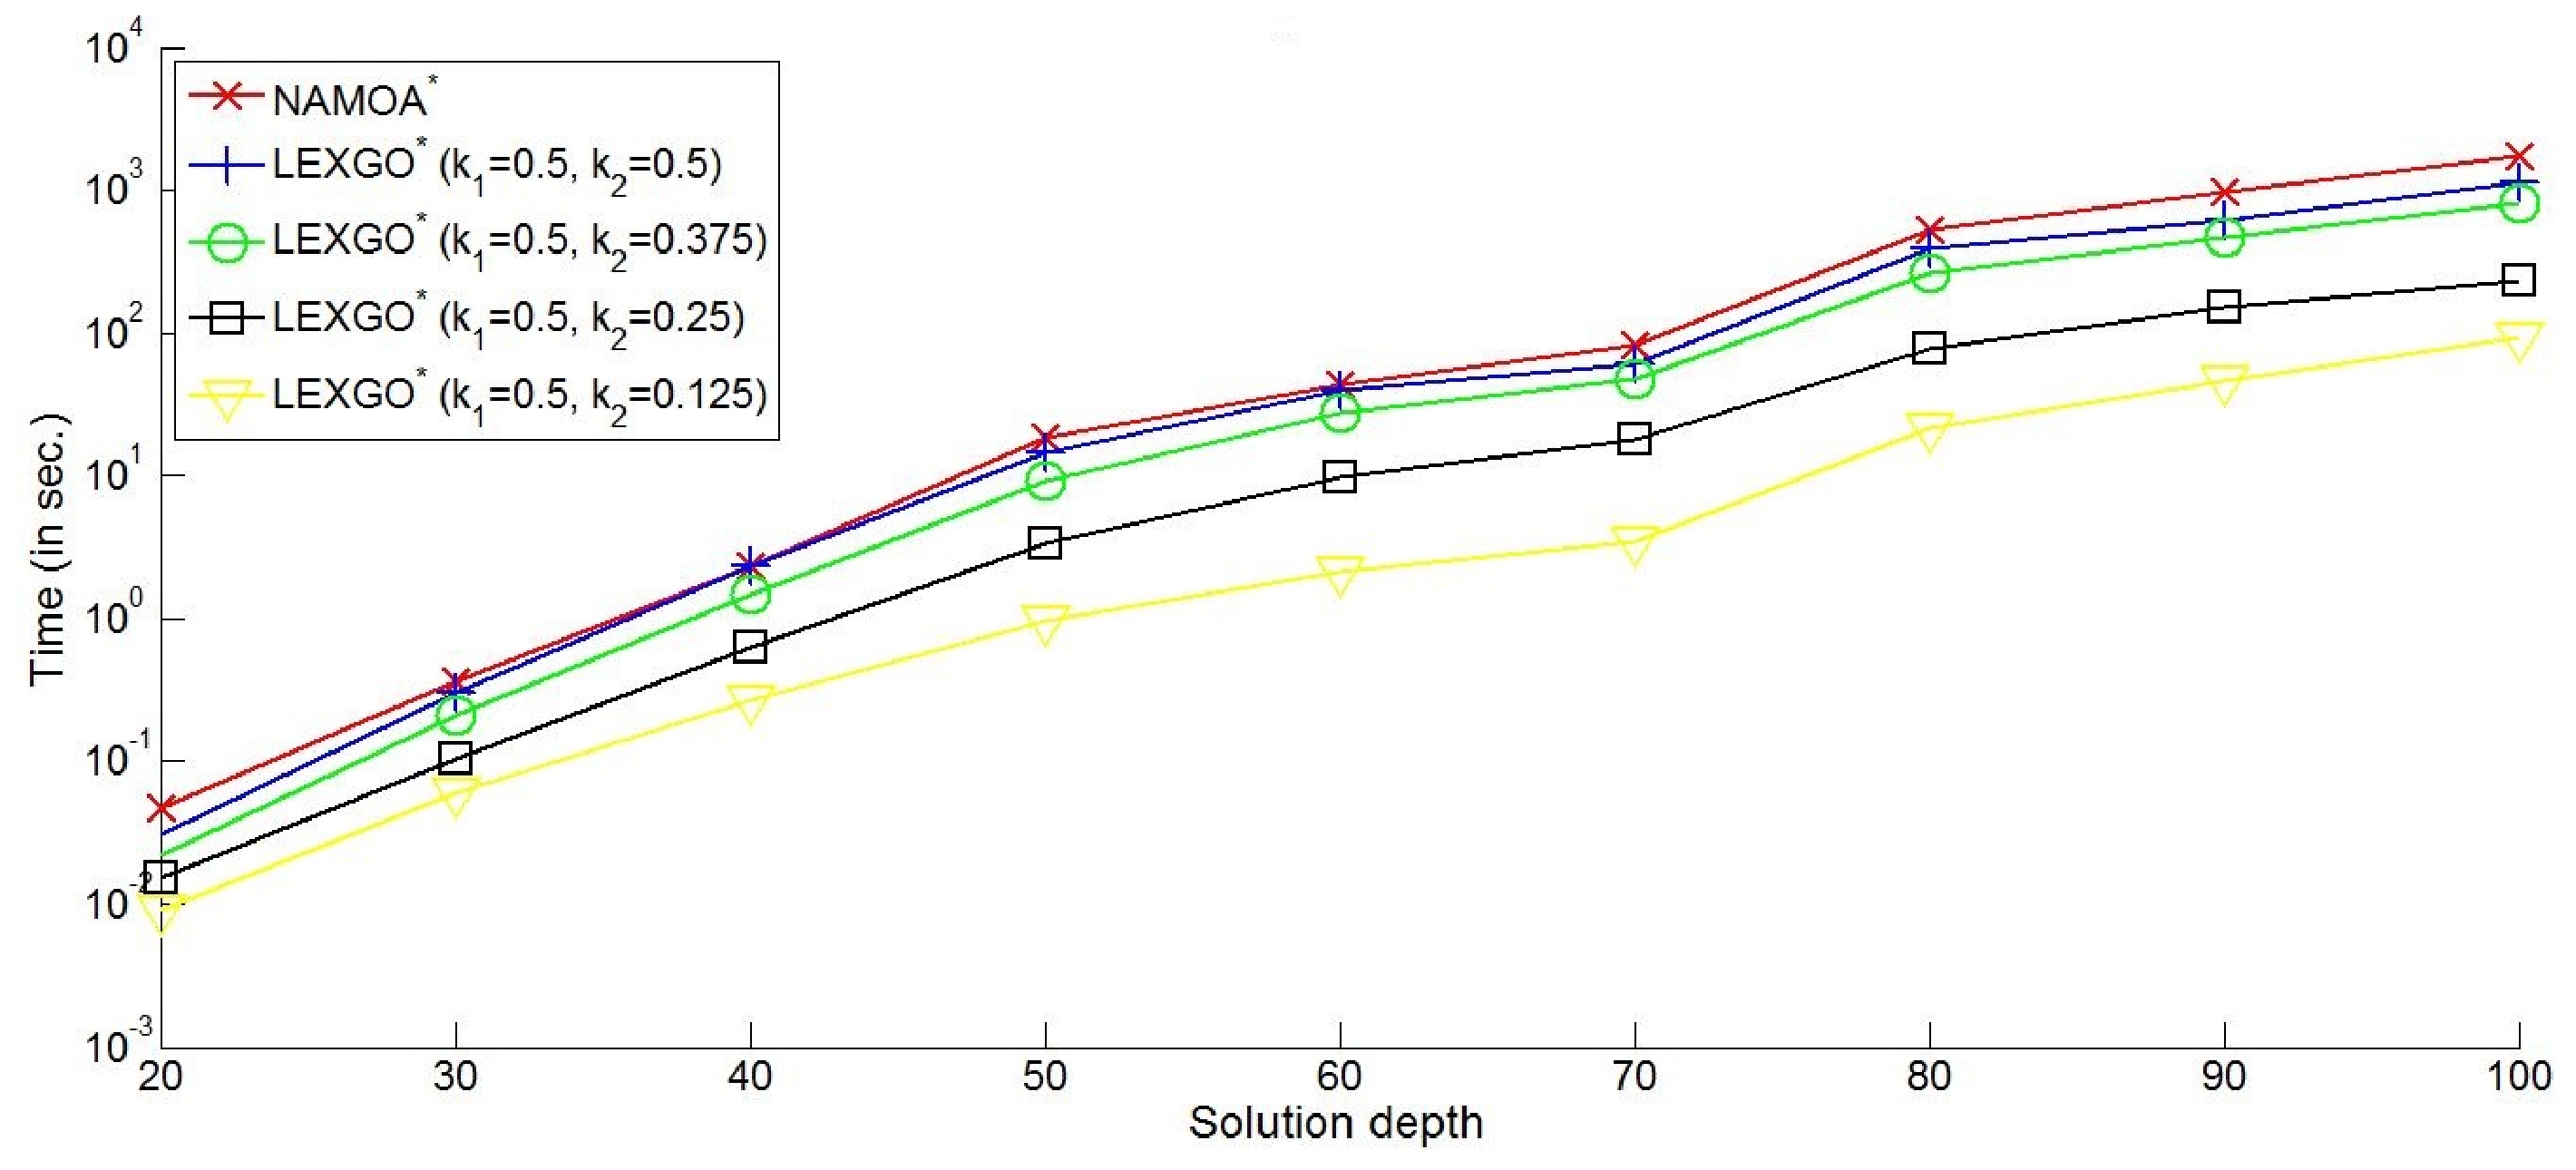
\includegraphics[width=0.95\textwidth]{Images/Chapter6/class2-exe05-lin}
        }\\ %  ------- End of the first row ----------------------%
    \end{center}
    \vspace{-0.25in} 
    \caption{%
Class II experiments on grids, average runtime (in seconds) per solution depth for \lexgo \ and \namoa \ with linear aggregation selection order. 
    }%
    \label{fig:6-6}
\end{figure}

A progressive reduction in scanned labels and runtimes is observed as the value of $k_2$ decreases. For $d=100$ and $k_2=0.75$, \lexgo \ explores around 97\% of labels explored by \namoa, but for $k_2=0.1875$ this value drops to only around 17.5\%. Similarly, when $k_2=0.5$ \ \lexgo explores around 60\% of labels explored by \namoa, but for $k_2=0.125$ this value falls to around 12\%. The percentage of Pareto goal-optimal solution costs returned also drops sharply as $k_2$ decreases. For $k_1=0.5$ and $k_2=0.125$, some problem instances could not satisfy all goals. 

Regarding the differences between the lexicographic and linear selection orders, we observed a better comparative performance of \lexgolex when compared to \namoalex \ than \lexgolin \ to \namoalin. The linear order introduces a particular case when $k_1=0.75$ and $k_2=0.5625$, since its runtime performance is worse than $k_1=0.75$ and $k_2=0.75$. The former performs a smaller number of label expansions but a much higher number of deviation pruning comparisons than the latter.

%-------------------------------------------------------------------
\subsection{Analysis on the pruning condition}
\label{chapEmpiricalAnalysis:subsec:analysisgridspruning}
%-------------------------------------------------------------------

Figures \ref{fig:6-7} and \ref{fig:6-8} compare average runtimes and scanned labels by \lexgo, with lexicographic selection order, with and without deviation pruning (see Equation \ref{eq:cond-prune-new}), respectively. Only the results with the lexicographic order are shown, since the results with the linear order are practically identical. These are results for the first set of experiments and $k_1 = 0$, where goals are not satisfied and deviation pruning is most effective. Values for \namoa \ are also displayed as reference. As soon as goals are satisfied, deviation pruning loses pruning power. For $k_1 = 0.25$ a smaller advantage is achieved. For larger values of $k_1$, deviation pruning does not offer practical advantage.

These results show where goals could be satisfied, i.e. $k_1 = \{0.5, 0.75, 1 \}$, deviation pruning does not improve performance in practice. However, for those values of $k_1$, i.e. $k_1 = \{0, 0.25\}$, where goals cannot be satisfied, deviation pruning can make a difference, specially for $k_1 = 0$. Figure \ref{fig:6-8} shows up to three orders of magnitude of improvement in runtime, that can be attributed to a reduction of two orders of magnitude in scanned labels (see Figure \ref{fig:6-7}). This can be explained by the fact that when goals are satisfied, values of deviation vectors of expanded labels are $\vec 0$ and deviation pruning is barely triggered. On the other hand, unsatisfied goals cause greater deviation values and hence, a greater number of pruning opportunities. Therefore, the higher deviation from goals, the more effective deviation pruning.  

\begin{figure}
\centering
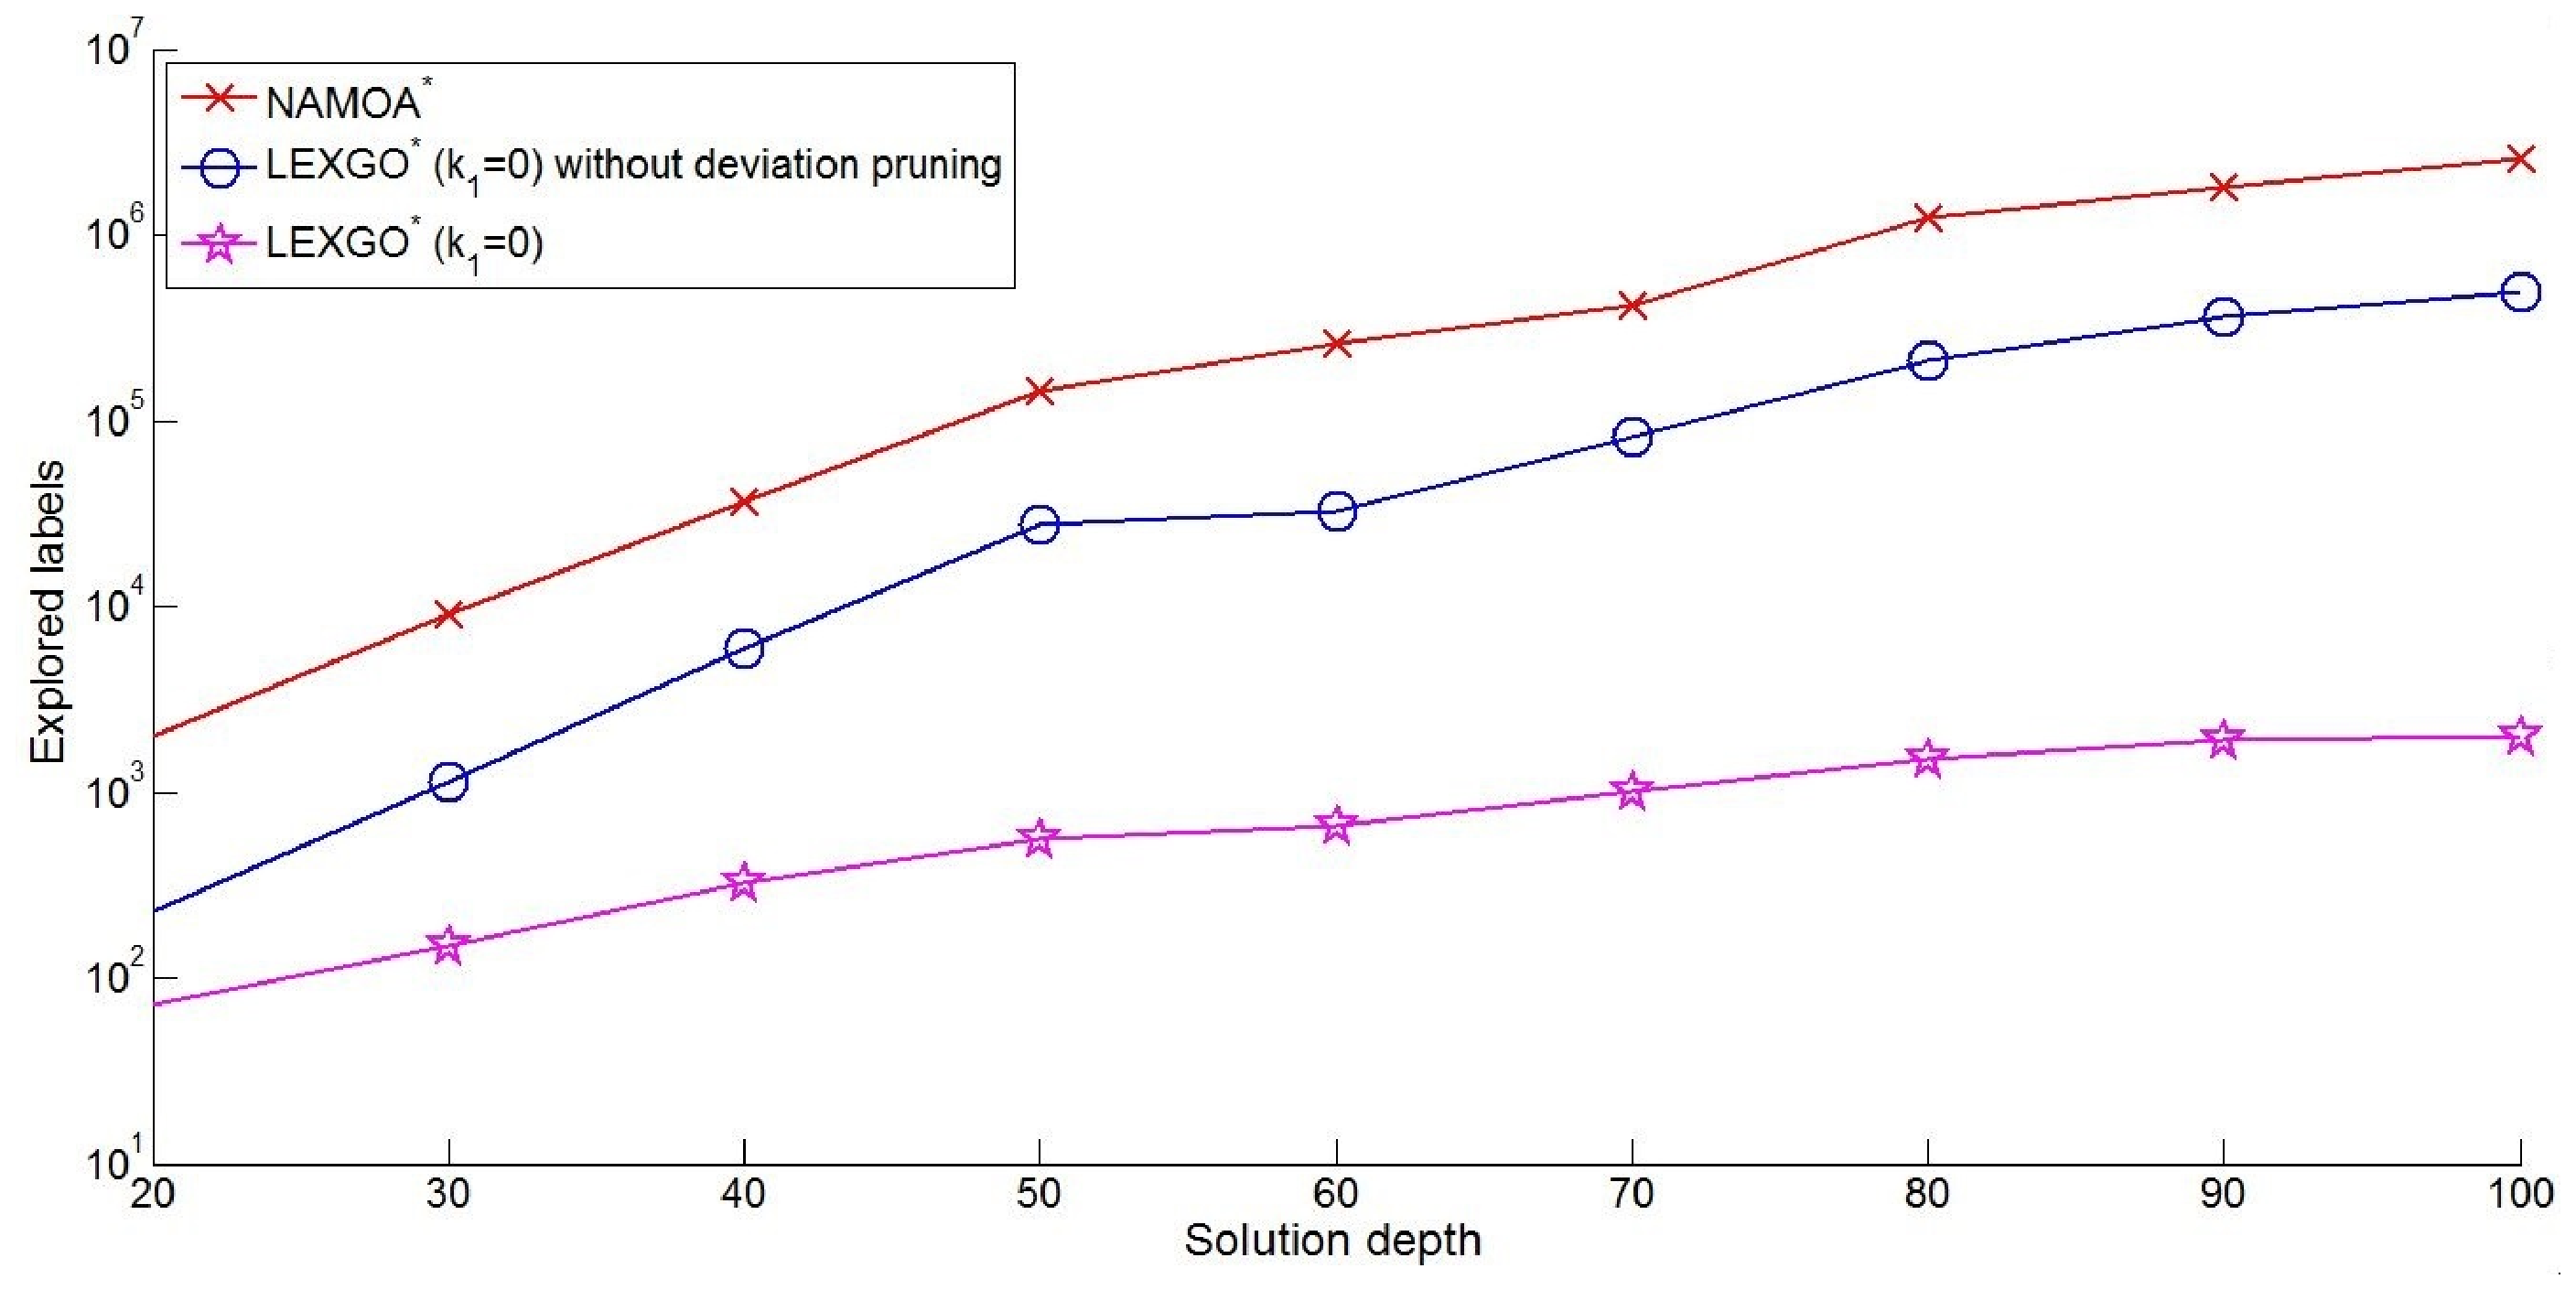
\includegraphics[width=1\textwidth]{Images/Chapter6/dev-pruning-labels0}
\caption{Class I experiments on grids, average explored labels per solution depth to \lexgo \ $(k_1 = 0)$ with and without deviation pruning.}
\label{fig:6-7}
\end{figure}

\begin{figure}
\centering
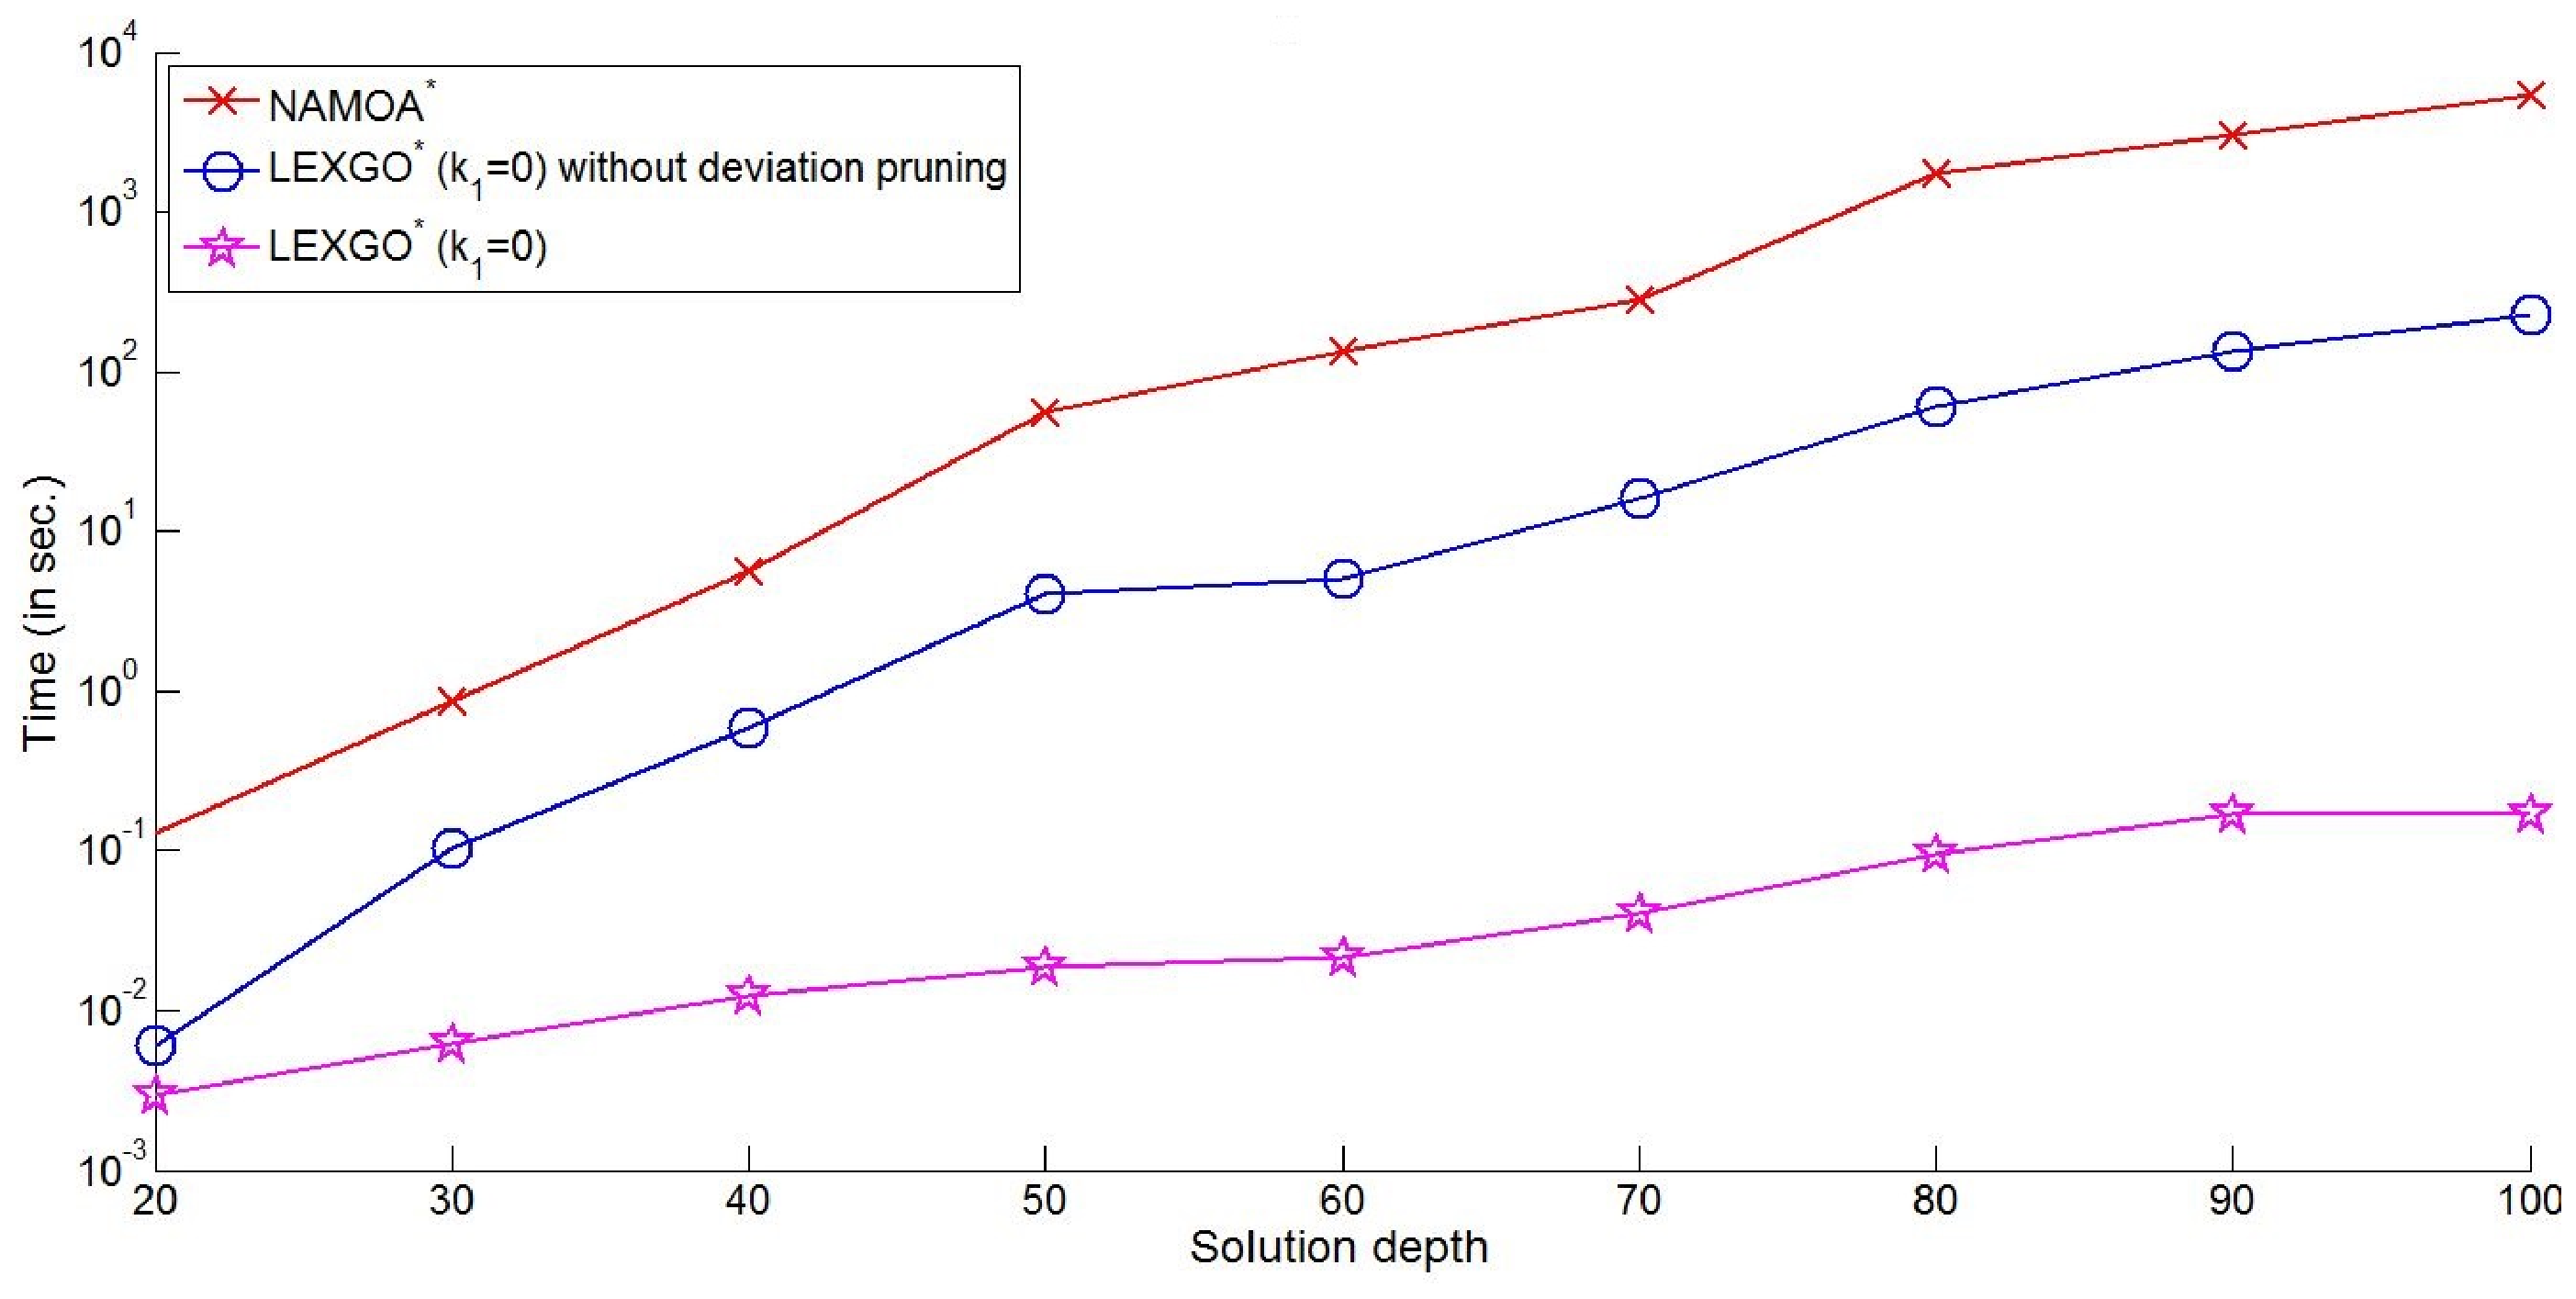
\includegraphics[width=1\textwidth]{Images/Chapter6/dev-pruning-exe0}
\caption{Class I experiments on grids, average runtimes in seconds per solution depth to \lexgo \ $(k_1 = 0)$ with and without deviation pruning.}
\label{fig:6-8}
\end{figure}

%-------------------------------------------------------------------
\subsection{Summary}
\label{chapEmpiricalAnalysis:subsec:summarygridslexgo}
%-------------------------------------------------------------------

We present a deeper study than the experiments already presented by the author in \citet{Pulido2014}. We have also added to the experimental set the linear aggregation order to both algorithms, \namoa \ and \lexgo, as well as $k_1=0.75$ for class II experiments. \namoalin \ outperforms \namoalex \ in all cases, by approximately a factor of two. Several studies have reported the same results for \namoa \ on the lexicographic and linear selection orders.  

Regarding \lexgolex \ and \lexgolin, the latter performs faster when the number of goal-optimal solution costs is bigger, i.e. when $k_1=\{1, 0.75\}$, by an approximate factor of 1.8, due to the fact that linear version finds the solutions at a later stage and therefore, a smaller number of filtering comparisons is needed. However, \lexgolex \ outperforms \lexgolin \ when the number of goal-optimal solution vectors is smaller, i.e. when $k_1=0.5$. Moreover, \lexgolex \ has a slightly better performance when goals cannot be satisfied, i.e. when $k_1=\{0.25, 0\}$. In the latter case, the relative performance is problem-dependent.

The comparative performance between \lexgolex \ vs \namoalex, and \lexgolin \ vs \namoalin \ turns out to be very similar in explored labels. However, the lexicographic order is comparatively more advantageous in runtime for \lexgo \ than the linear, having a smaller time overhead and better comparative performance. Even so, both \lexgo \ alternatives run faster than \namoa \ for $k_1=0.5$, they run several orders of magnitude faster for $k_1=0$ and around two orders of magnitude when $k_1=0.25$, regardless the selection order. 

%-------------------------------------------------------------------
\section{\texorpdfstring{\namoate}{NAMOA*dr} \ vs \texorpdfstring{\namoa}{NAMOA*}}
\label{chapEmpiricalAnalysis:sec:resultsgridsnamoate}
%-------------------------------------------------------------------

In this section, we analyze the runtime performance of two different versions of the \namoa \ algorithm: the standard version, and the newly introduced one. A description of these algorithms can be found in Sections \ref{chapMultiObjAlg:subsec:namoa} and \ref{chapMultiObjAlg:subsec:namoate}, respectively. \namoa \ and \namoate \ were presented in Section \ref{chapMultiObjAlg:subsec:namoa} and Section \ref{chapMultiObjAlg:subsec:namoate}, respectively. 

The experiments presented in this section analyze the impact of the dimensionality reduction technique on the sets of random grid problems previously used with $q=3$. Extra problem sets with $q=4$ and $q=5$ objectives have been added to the experimental evaluation of these algorithms. The solution depths considered for these new experiments are $d = \{20, 30, 40, 50 \}$ and $d = \{20, 30, 40 \}$ for $q=4$ and $q=5$, respectively.

These two versions of \namoa \ differ in the order of selection of OPEN labels and in the way dominance is checked in filtering and cl-pruning operations. The first analyzed variants are \namoalex \ and \namoalin, which use, to the best of our knowledge, the usual dominance pruning and filtering techniques in previously reported experimental evaluations of multiobjective search algorithms. The second algorithm analyzed, \namoate \ uses a lexicographic order of selection and the t-discarding technique for filtering and cl-pruning, as described in Section \ref{chapMultiObjAlg:sec:Time-efficient-MSalg}.

%-------------------------------------------------------------------
\subsection{Analysis}
\label{chapEmpiricalAnalysis:subsec:analysisgridsnamoate}
%-------------------------------------------------------------------

Table \ref{tab:6-6} shows the average size of relevant sets of labels for the execution of \namoate \ on random grid problems. The first column ($q$) indicates the number of objectives. The second column ($d$) displays solution depth. The third column (Max OPEN) displays the maximum cardinality of the set of open labels. The fourth column, $\sum G_{cl}$, displays the total number of closed (permanent) labels at termination, calculated as the sum of the number of labels at the $G_{cl}$ sets of all visited nodes. This is also the total number of labels expanded by the algorithm. The fifth column shows for comparison the sum of sizes of the corresponding sets of truncated labels, i.e. $\sum T(G_{cl})$. The sixth column displays the percentage ratio between columns four and five. For example, for $d = 20$, the average number of label expansions by \namoate \ was 1,985, while the average number of labels in the truncated sets was only 476, this results in a percentage ratio of 23.98\%.   

\begin{table}
\caption{Average size of relevant sets of labels for random grid problems solved by \namoate.}
\begin{center}
\begin{tabular}{crrrrrrrr}
\hline \noalign{\smallskip}
$q$ & $d$ & Max OPEN & $\sum G_{cl}$ & $\sum T(G_{cl})$ & \% & $\text{C}^*$ & $T(\text{C}^*)$ & \%\\
\noalign{\smallskip} \hline 
3 & 20  & 194    & 1,985     & 476    & 23.98 & 122   & 13  & 10.66 \\
3 & 30  & 723    & 9,164     & 2,091  & 22.82 & 302   & 32  & 10.60 \\
3 & 40  & 2,233  & 36,557    & 4,923  & 13.47 & 694   & 44  &  6.34 \\
3 & 50  & 8,327  & 145,823   & 12,450 &  8.54 & 1,599 & 60  &  3.75 \\
3 & 60  & 11,091 & 257,935   & 21,026 &  8.15 & 2,007 & 80  &  3.99 \\
3 & 70  & 17,312 & 420,056   & 29,845 &  7.11 & 2,561 & 74  &  2.89 \\
3 & 80  & 38,512 & 1,231,565 & 61,457 &  4.99 & 5,423 & 108 &  1.99 \\
3 & 90  & 51,817 & 1,789,607 & 81,036 &  4.53 & 5,912 & 122 &  2.06 \\
3 & 100 & 72,062 & 2,550,354 & 97,160 &  3.81 & 8,307 & 137 &  1.65 \\
\noalign{\smallskip}
4 & 20  & 531     & 6,192     & 2,061   & 33.28 & 493    & 83    & 16.83 \\
4 & 30  & 3,183   & 49,735    & 13,150  & 26.44 & 2,230  & 320   & 14.34 \\
4 & 40  & 14,409  & 283,811   & 44,191  & 15.57 & 7,826  & 774   &  9.89 \\
4 & 50  & 72,112  & 1,542,793 & 153,639 & 9.95  & 24,942 & 1,382 &  5.54 \\
\noalign{\smallskip}
5 & 20  & 1,127   & 15,681     & 6,539    & 41.70 & 1,819   & 522   & 28.69 \\
5 & 30  & 10,019  & 172,238    & 51,145   & 29.69 & 10,830  & 1,917 & 17.70 \\
5 & 40  & 62,280  & 1,371,885  & 319,333  & 23.27 & 49,634  & 8,320 & 16.76 \\
\hline
\end{tabular} 
\end{center}
\label{tab:6-6}
\end{table}

Column 7 in Table \ref{tab:6-6} shows the average number of different non-dominated solution vectors in COSTS ($\text{C}^*$). The eighth column displays the size of the corresponding truncated set $T(\text{C}^*)$. The last column displays the percentage ratio between columns six and seven. 

Table \ref{tab:6-7} displays the average runtimes of the three considered alternatives of \namoa \ with $q \in \{3,4,5\}$ objectives for random grid problems. The last columns show the relative percentage improvement of \namoate \ over \namoalex \ and \namoalin, respectively.

\begin{table}
\caption{Average runtimes in seconds for random grid problems.}
\begin{center}
\scalebox{.80}{
\begin{tabular}{crrrrrrrrr}
\hline \noalign{\smallskip}
$q$ & $d$ & \namoalex & $\sigma_{lex}$ & \namoalin & $\sigma_{lin}$ & \namoate & $\sigma_{dr}$ & $(\frac{dr}{lex})$\% & $(\frac{dr}{lin})$\% \\
\noalign{\smallskip} \hline 
3 & 20  & 0.06  & 0.02    & 0.04  & 0.01 & 0.0622  & 0.01 & 99.67 & 132.91 \\
3 & 30  & 0.46   & 0.26     & 0.36   & 0.18 & 0.293    & 0.11 & 62.74 & 80.23 \\
3 & 40  & 3.53    & 1.21     & 2.36    & 0.74 & 1.32     & 0.30 & 37.39 & 56.13 \\
3 & 50  & 36.83   & 15.56    & 18.37   & 5.67 & 6.87     & 2.02 & 18.65 & 37.41 \\
3 & 60  & 86.93   & 49.57    & 43.83   & 22.94 & 11.94   & 4.48 & 13.73 & 27.26 \\
3 & 70  & 178.53  & 106.75   & 83.37   & 47.77 & 20.93   & 7.69 & 11.72 & 25.11 \\
3 & 80  & 1,164.11 & 293.72   & 533.79  & 135.96 & 76.01  & 14.22 & 6.52 & 14.24 \\
3 & 90  & 2,030.06 & 730.05   & 981.32  & 313.79 & 120.66 & 33.19 & 5.94 & 12.30 \\
3 & 100 & 3,662.93 & 1,100.91 & 1,754.43 & 583.28 & 196.13 & 52.74 & 5.35 & 11.18 \\
\noalign{\smallskip}
4 & 20  & 0.39   & 0.14     & 0.30    & 0.11     & 0.23   & 0.07 & 58.52 & 76.66 \\    
4 & 30  & 11.64   & 4.22     & 8.88    & 3.87     & 4.31   & 1.97 & 37.02 & 48.53 \\     
4 & 40  & 292.17  & 188.27   & 166.36  & 105.31   & 50.41  & 29.47 & 17.25 & 30.30 \\     
4 & 50  & 5,604.29 & 2,356.35 & 3,173.81 & 1,171.11 & 645.37 & 195.84 & 11.51 & 20.33 \\
\noalign{\smallskip}
5 & 20  & 4.01     & 1.51     & 2.99     & 1.14     & 2.20    & 0.76 &  54.86 & 73.57 \\  
5 & 30  & 204.69   & 135.77   & 114.91   & 73.32    & 57.89   & 34.61 &  28.28 & 50.37 \\    
5 & 40  & 10,848.24 & 7,404.86 & 6,141.63  & 4,212.81 & 1,919.56 & 1,269.98 &  17.69 & 31.25 \\ 
\hline
\end{tabular} 
}
\end{center}
\label{tab:6-7}
\end{table} 

All evaluated algorithms perform op-pruning in the same way. However, \namoate \ uses a different technique for cl-pruning and filtering. Figure \ref{fig:6-9} displays some results of the execution of \namoate: the percentage of labels pruned by $G_{op}$ (op-pruning), truncated closed node labels $T(G_{cl})$ (cl-pruning), and filtered by  $T(\text{C}^*)$ over the total number of discarded labels. Results are displayed as a function of solution depth $d$, (a) for $q=3$ objectives, (b) for $q=4$ objectives, and (c) for $q=5$ objectives. 

\begin{figure}
    \begin{center}
%
      \subfigure[$q = 3$]{%
            \label{fig:6-9a}
        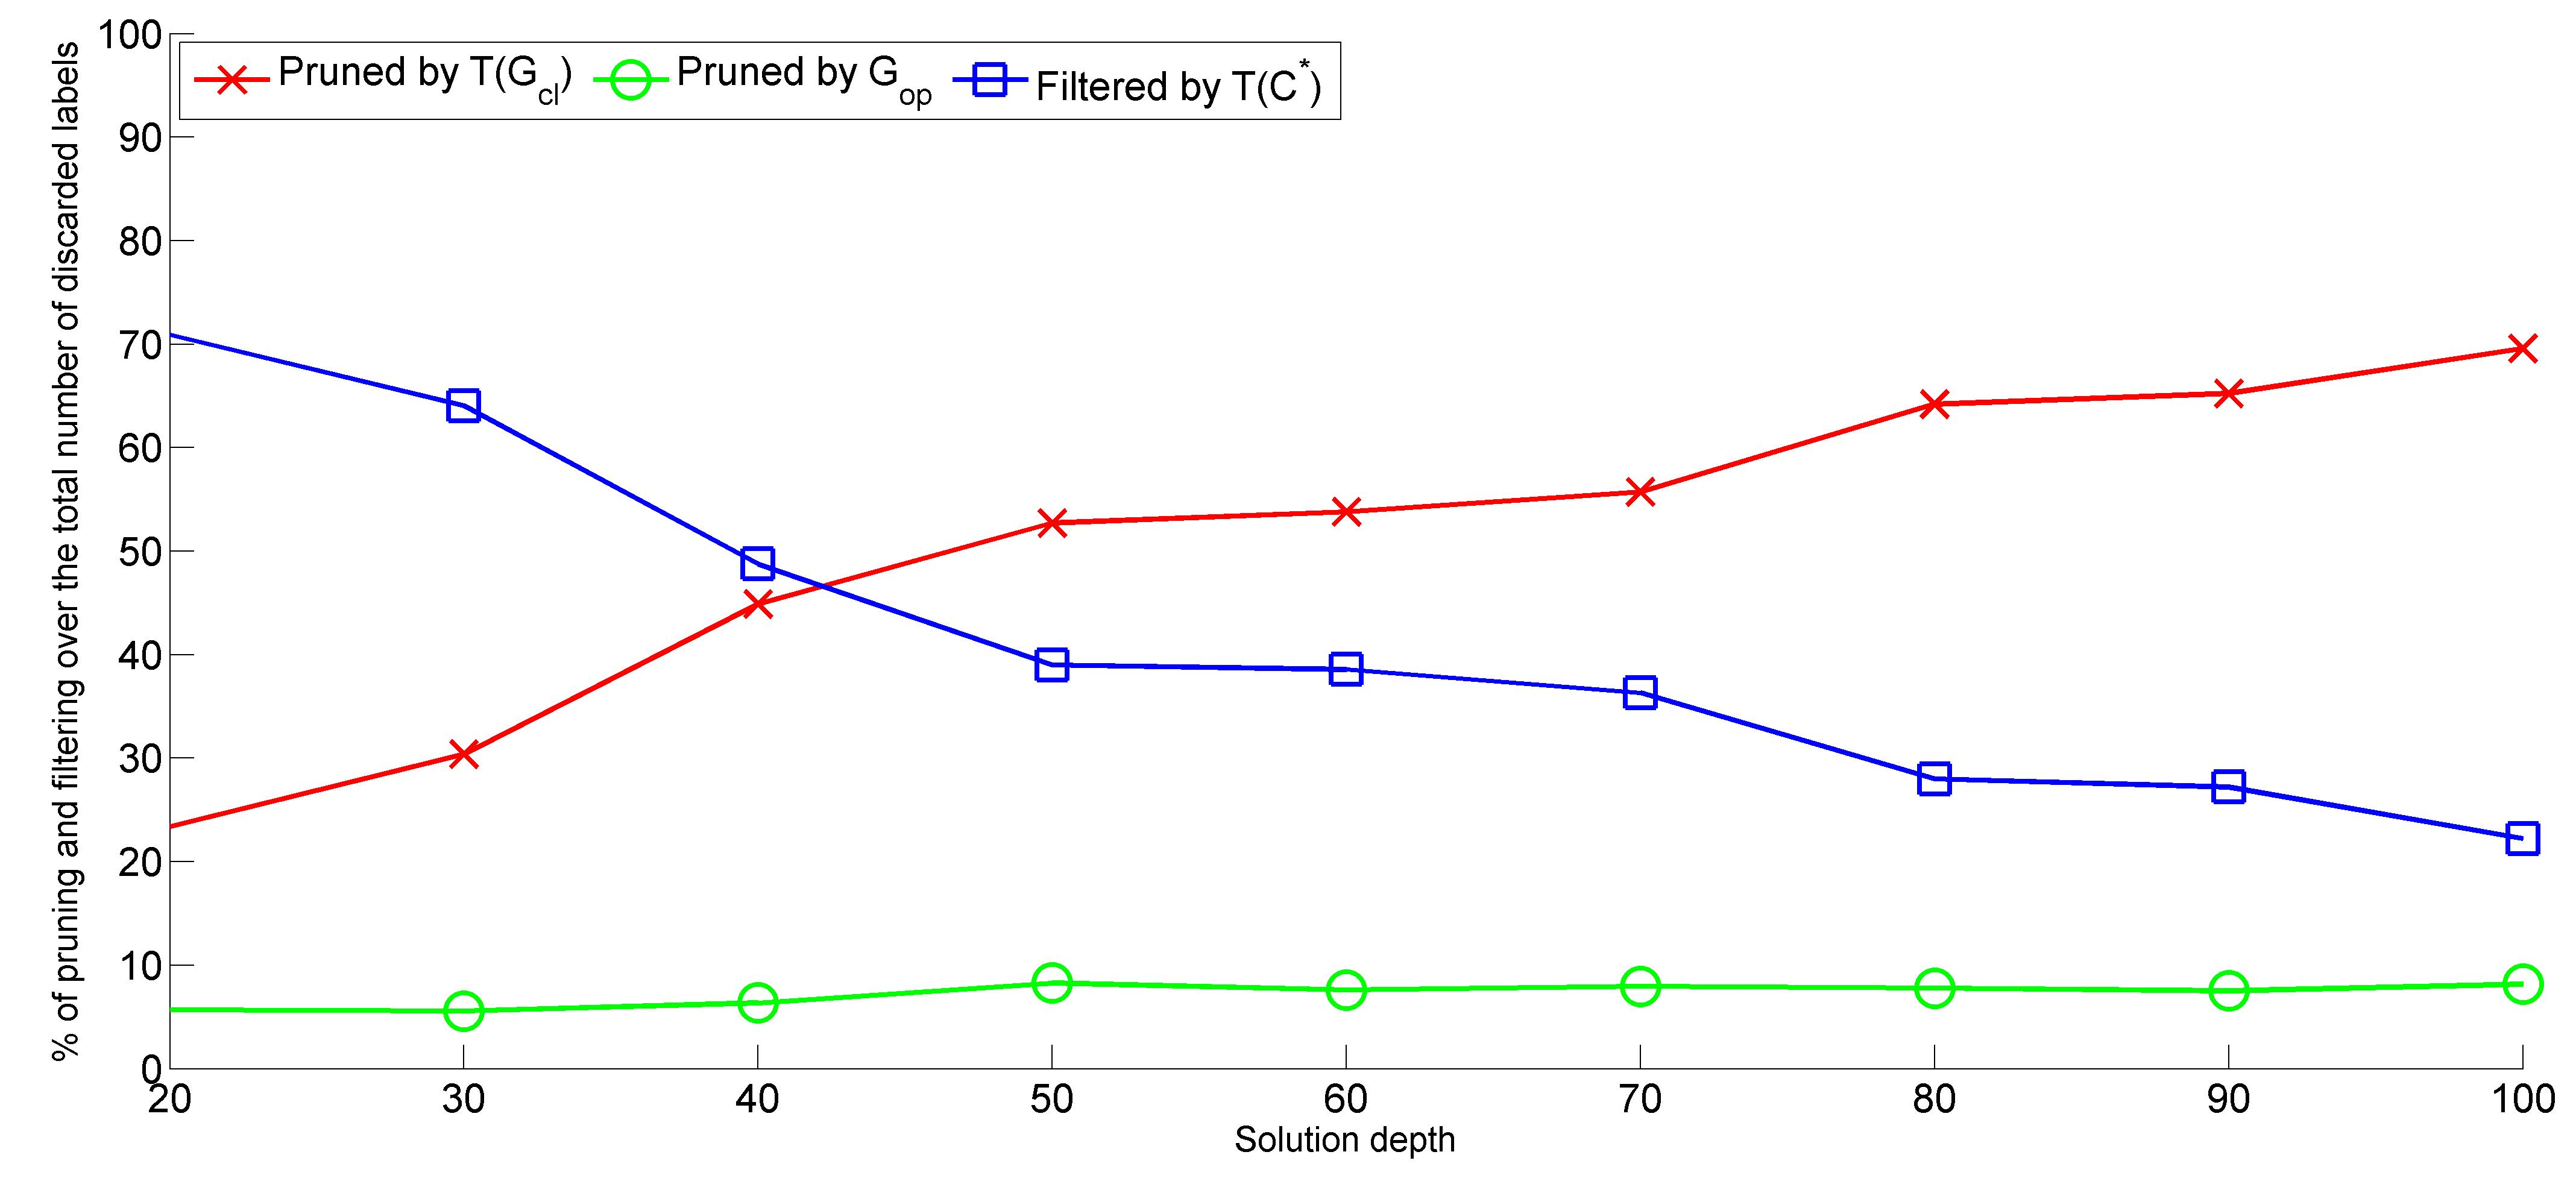
\includegraphics[width=0.95\textwidth]{Images/Chapter6/pruned-filtered-labels-grids-perc-a}
        }\\ %  ------- End of the first row ----------------------%
      \subfigure[$q = 
            4$]{%
       		\label{fig:6-9b}  
 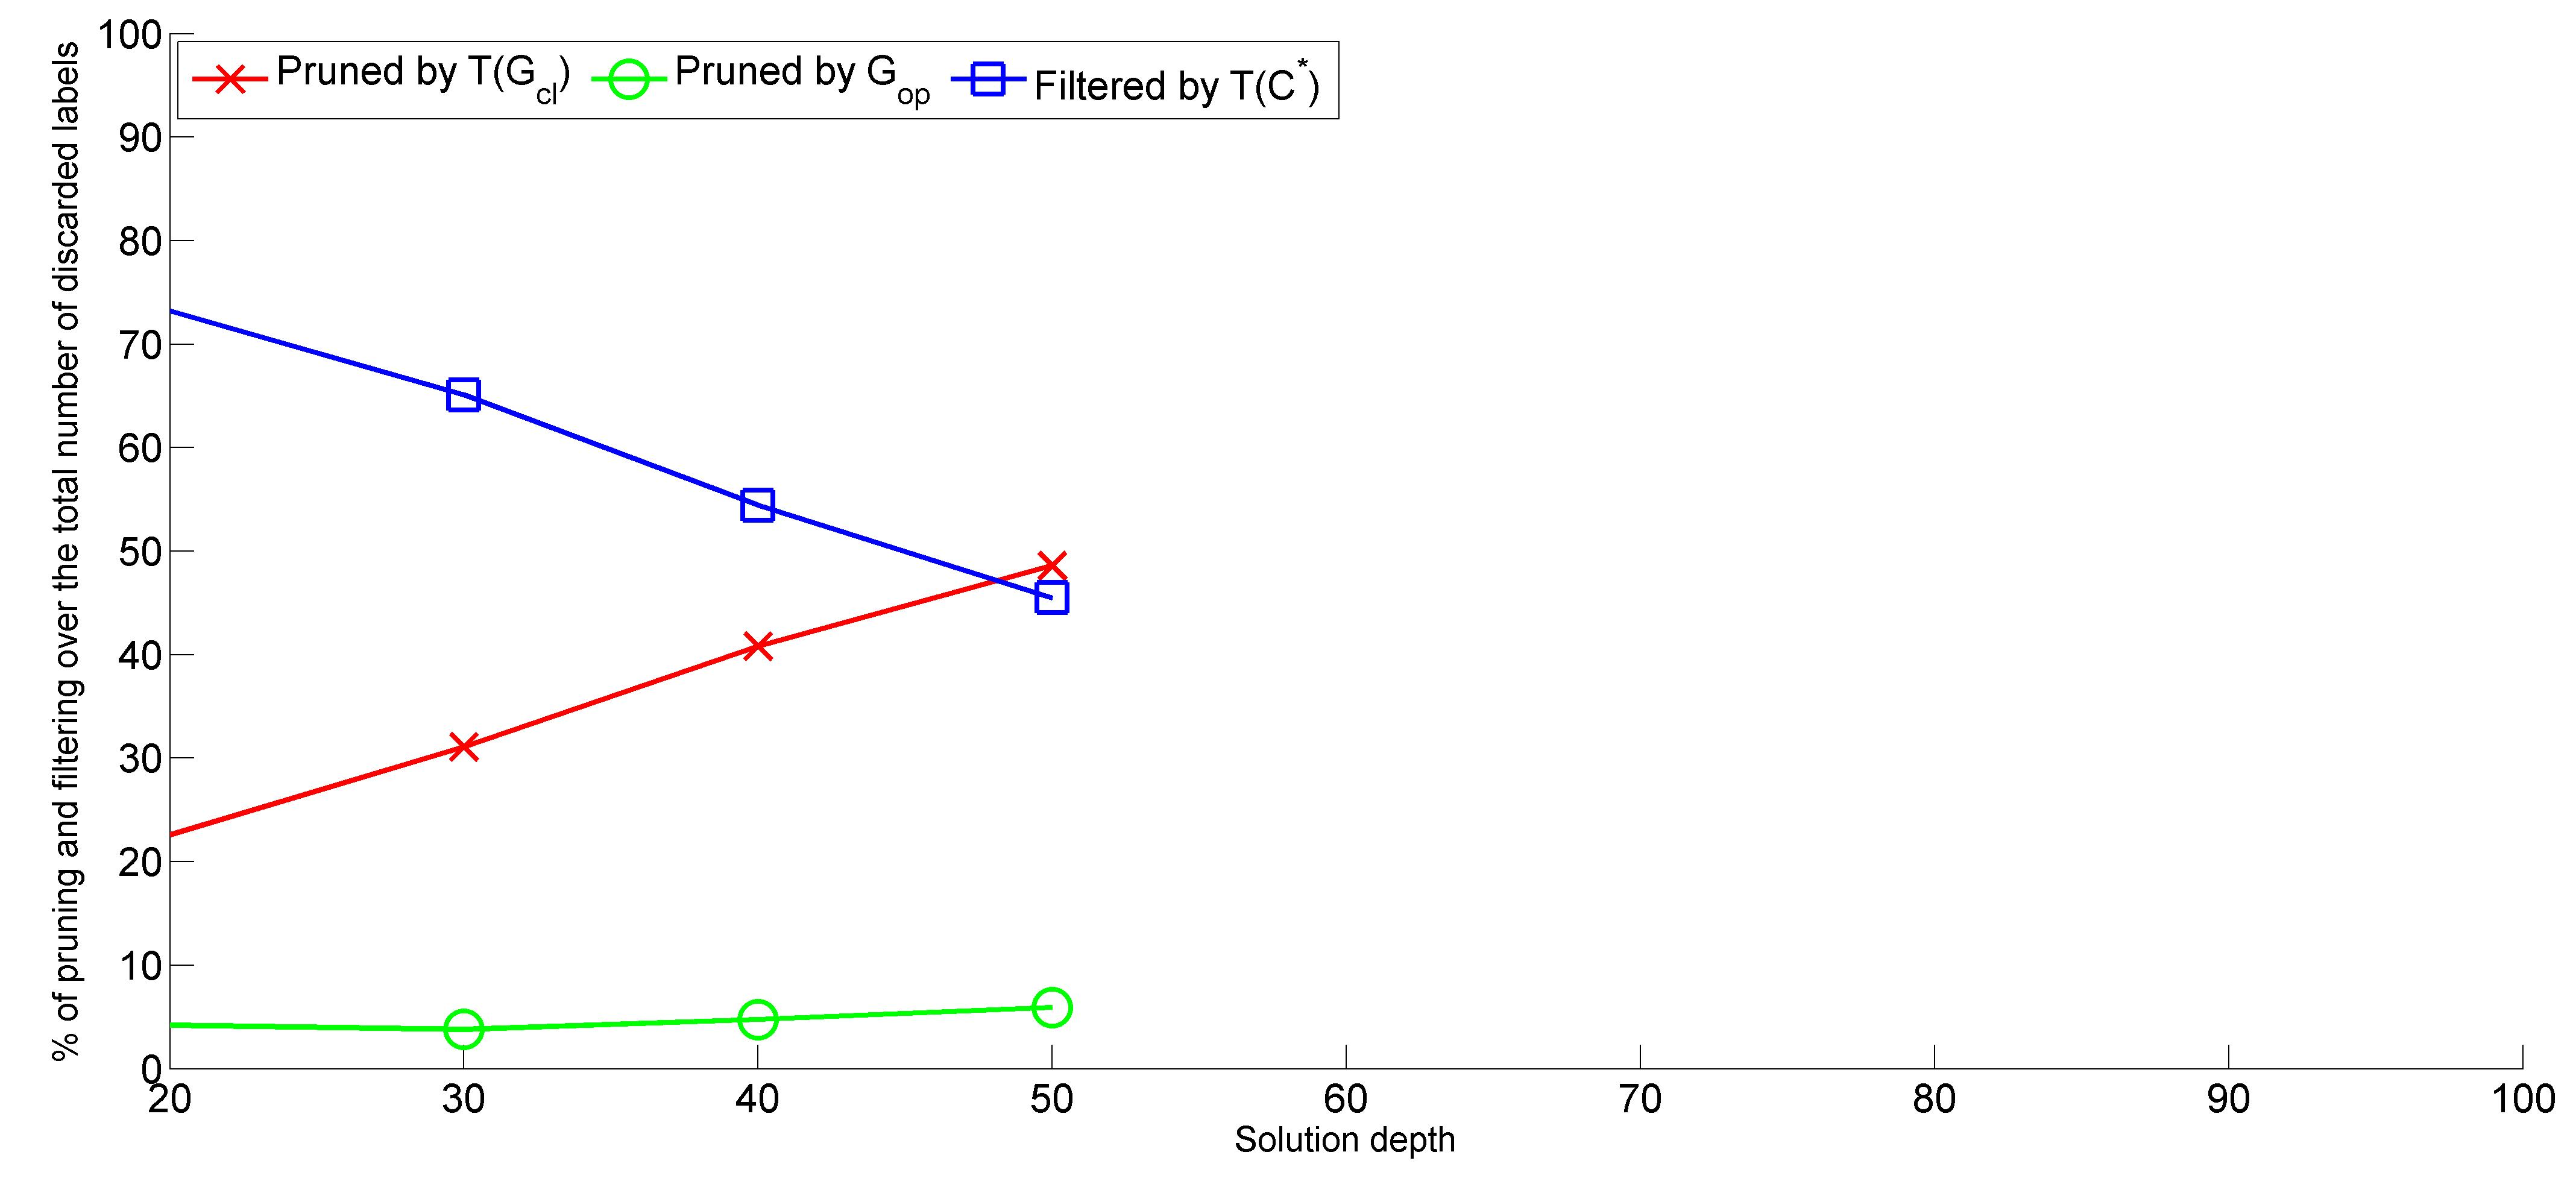
\includegraphics[width=0.95\textwidth]{Images/Chapter6/pruned-filtered-labels-grids-perc-b}
        }\\ %  ------- End of the first row ----------------------%
      \subfigure[$q = 5$]{%
            \label{fig:6-9c}
        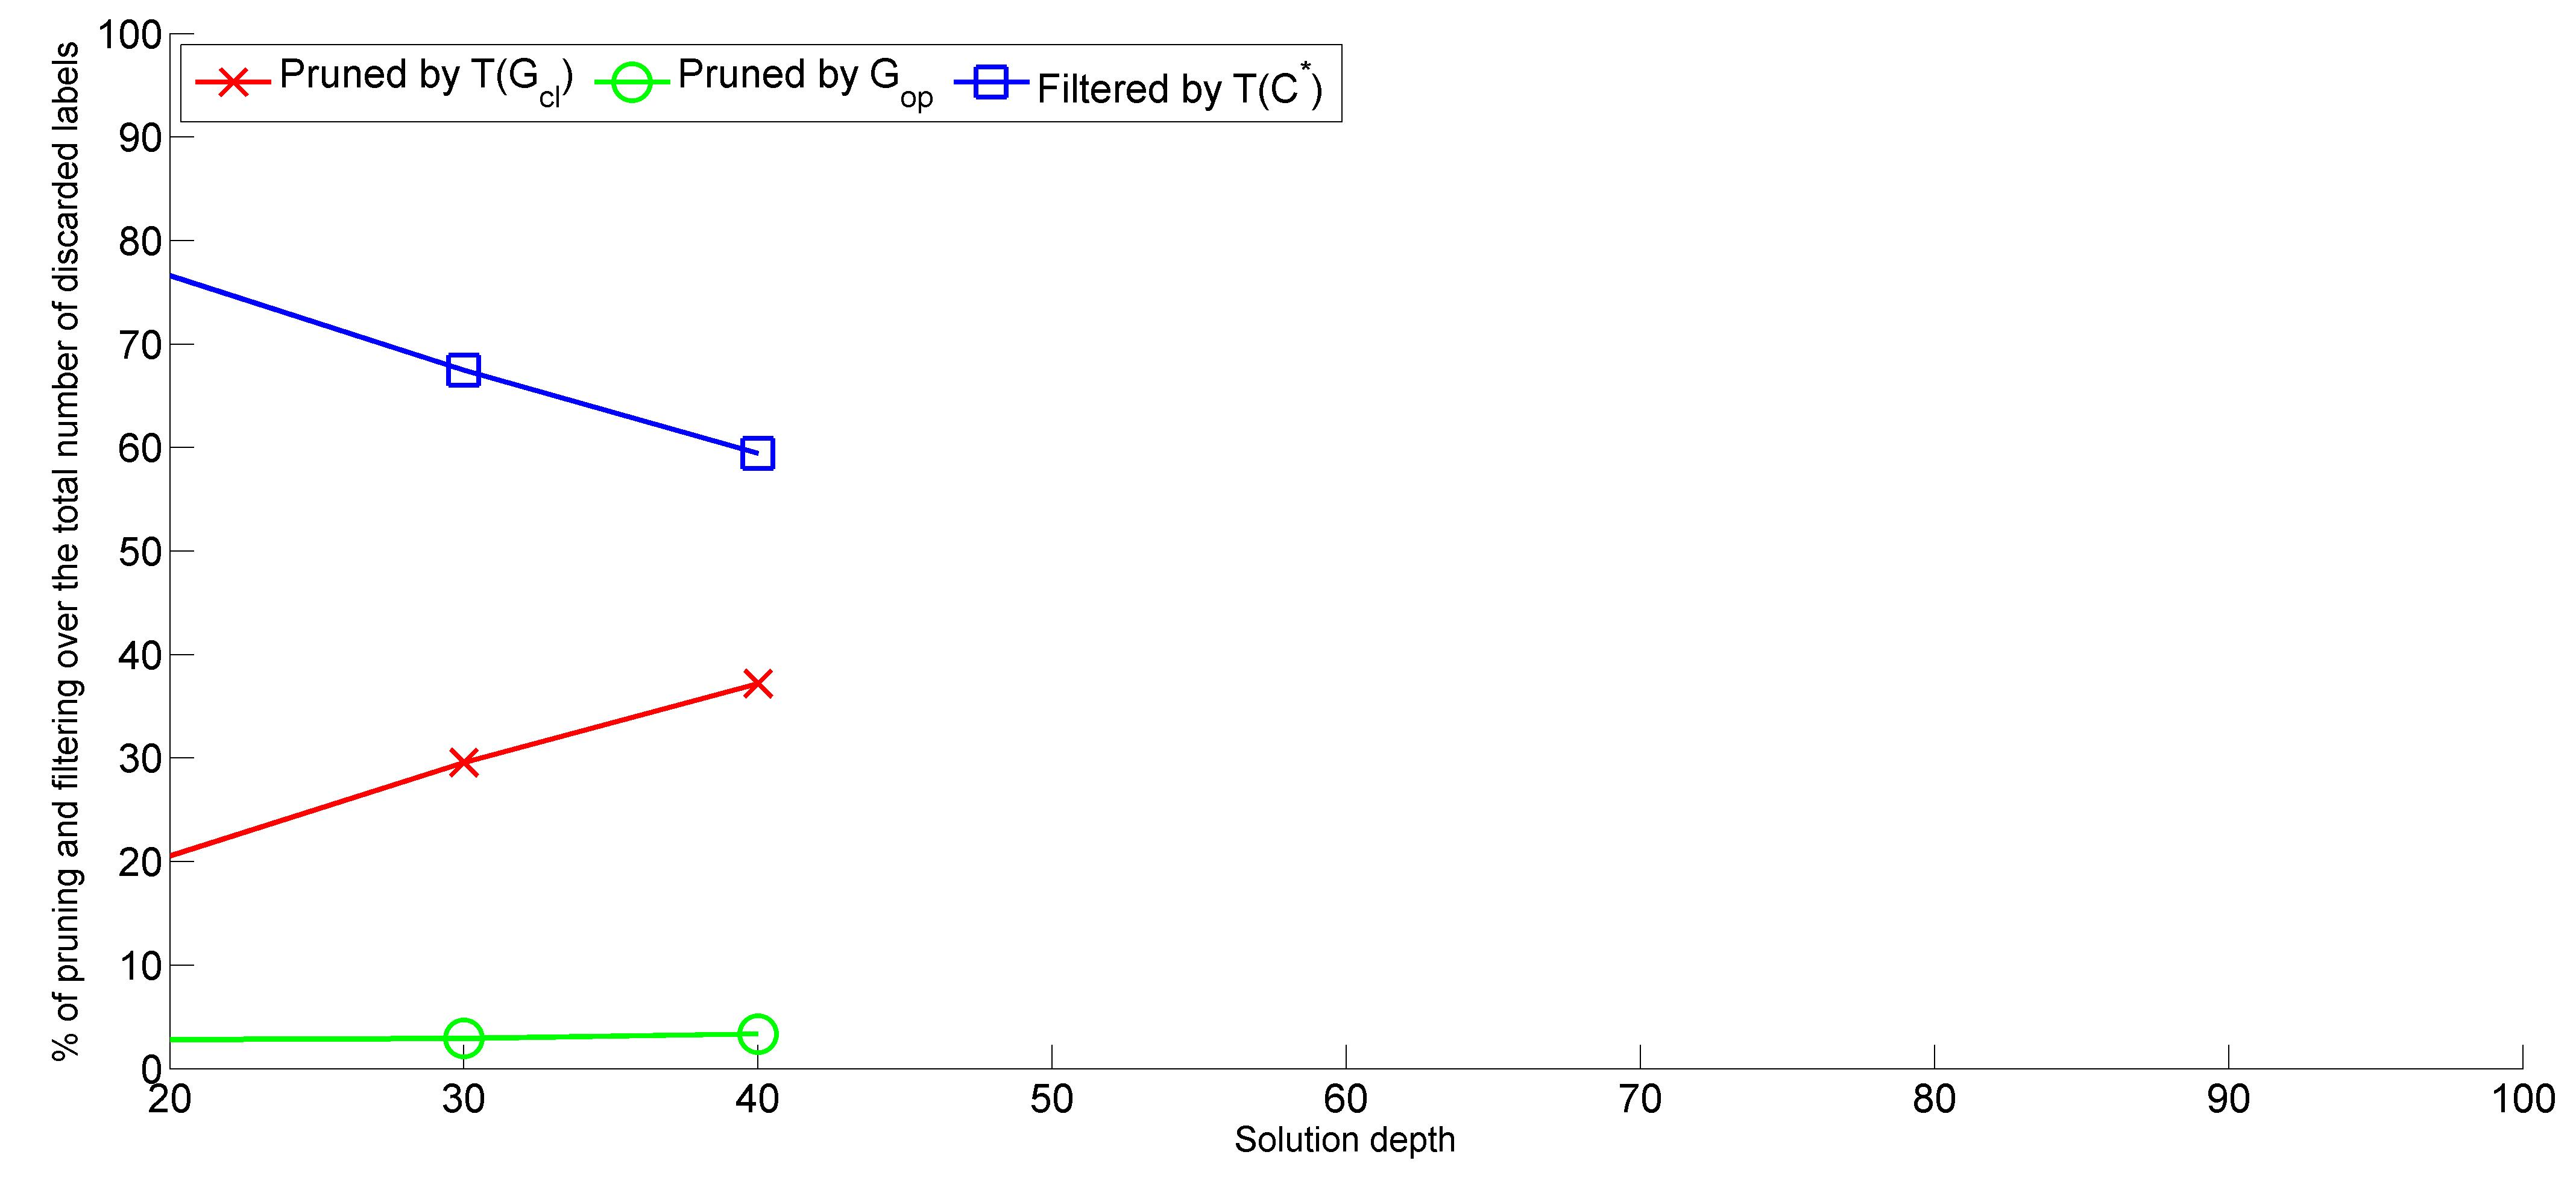
\includegraphics[width=0.95\textwidth]{Images/Chapter6/pruned-filtered-labels-grids-perc-c}
      }%
    \end{center}
    \vspace{-0.25in} 
    \caption{%
Percentage of pruned and filtered labels over the total number of discarded labels by \namoate \ per solution depth for $q \in \{3,4,5\}$ objectives in grid problems.  
    }%
    \label{fig:6-9}

\end{figure}

Figure \ref{fig:6-10} shows runtimes of \namoalex, \ \namoalin \ and \namoate \ in logarithmic scale against solution depth for $q=\{3,4,5\}$ objectives. The items in the legend indicate the version of the algorithm and the objectives, e.g. dr(4) indicates \namoate \ with $q=4$. Finally, Figure \ref{fig:6-11} displays the percentage of runtimes of \namoate \ and \namoalin \ over \namoalex \ for $q = 3$ experiments displayed as a function of solution depth. 

\begin{figure}%[ht]
\centering
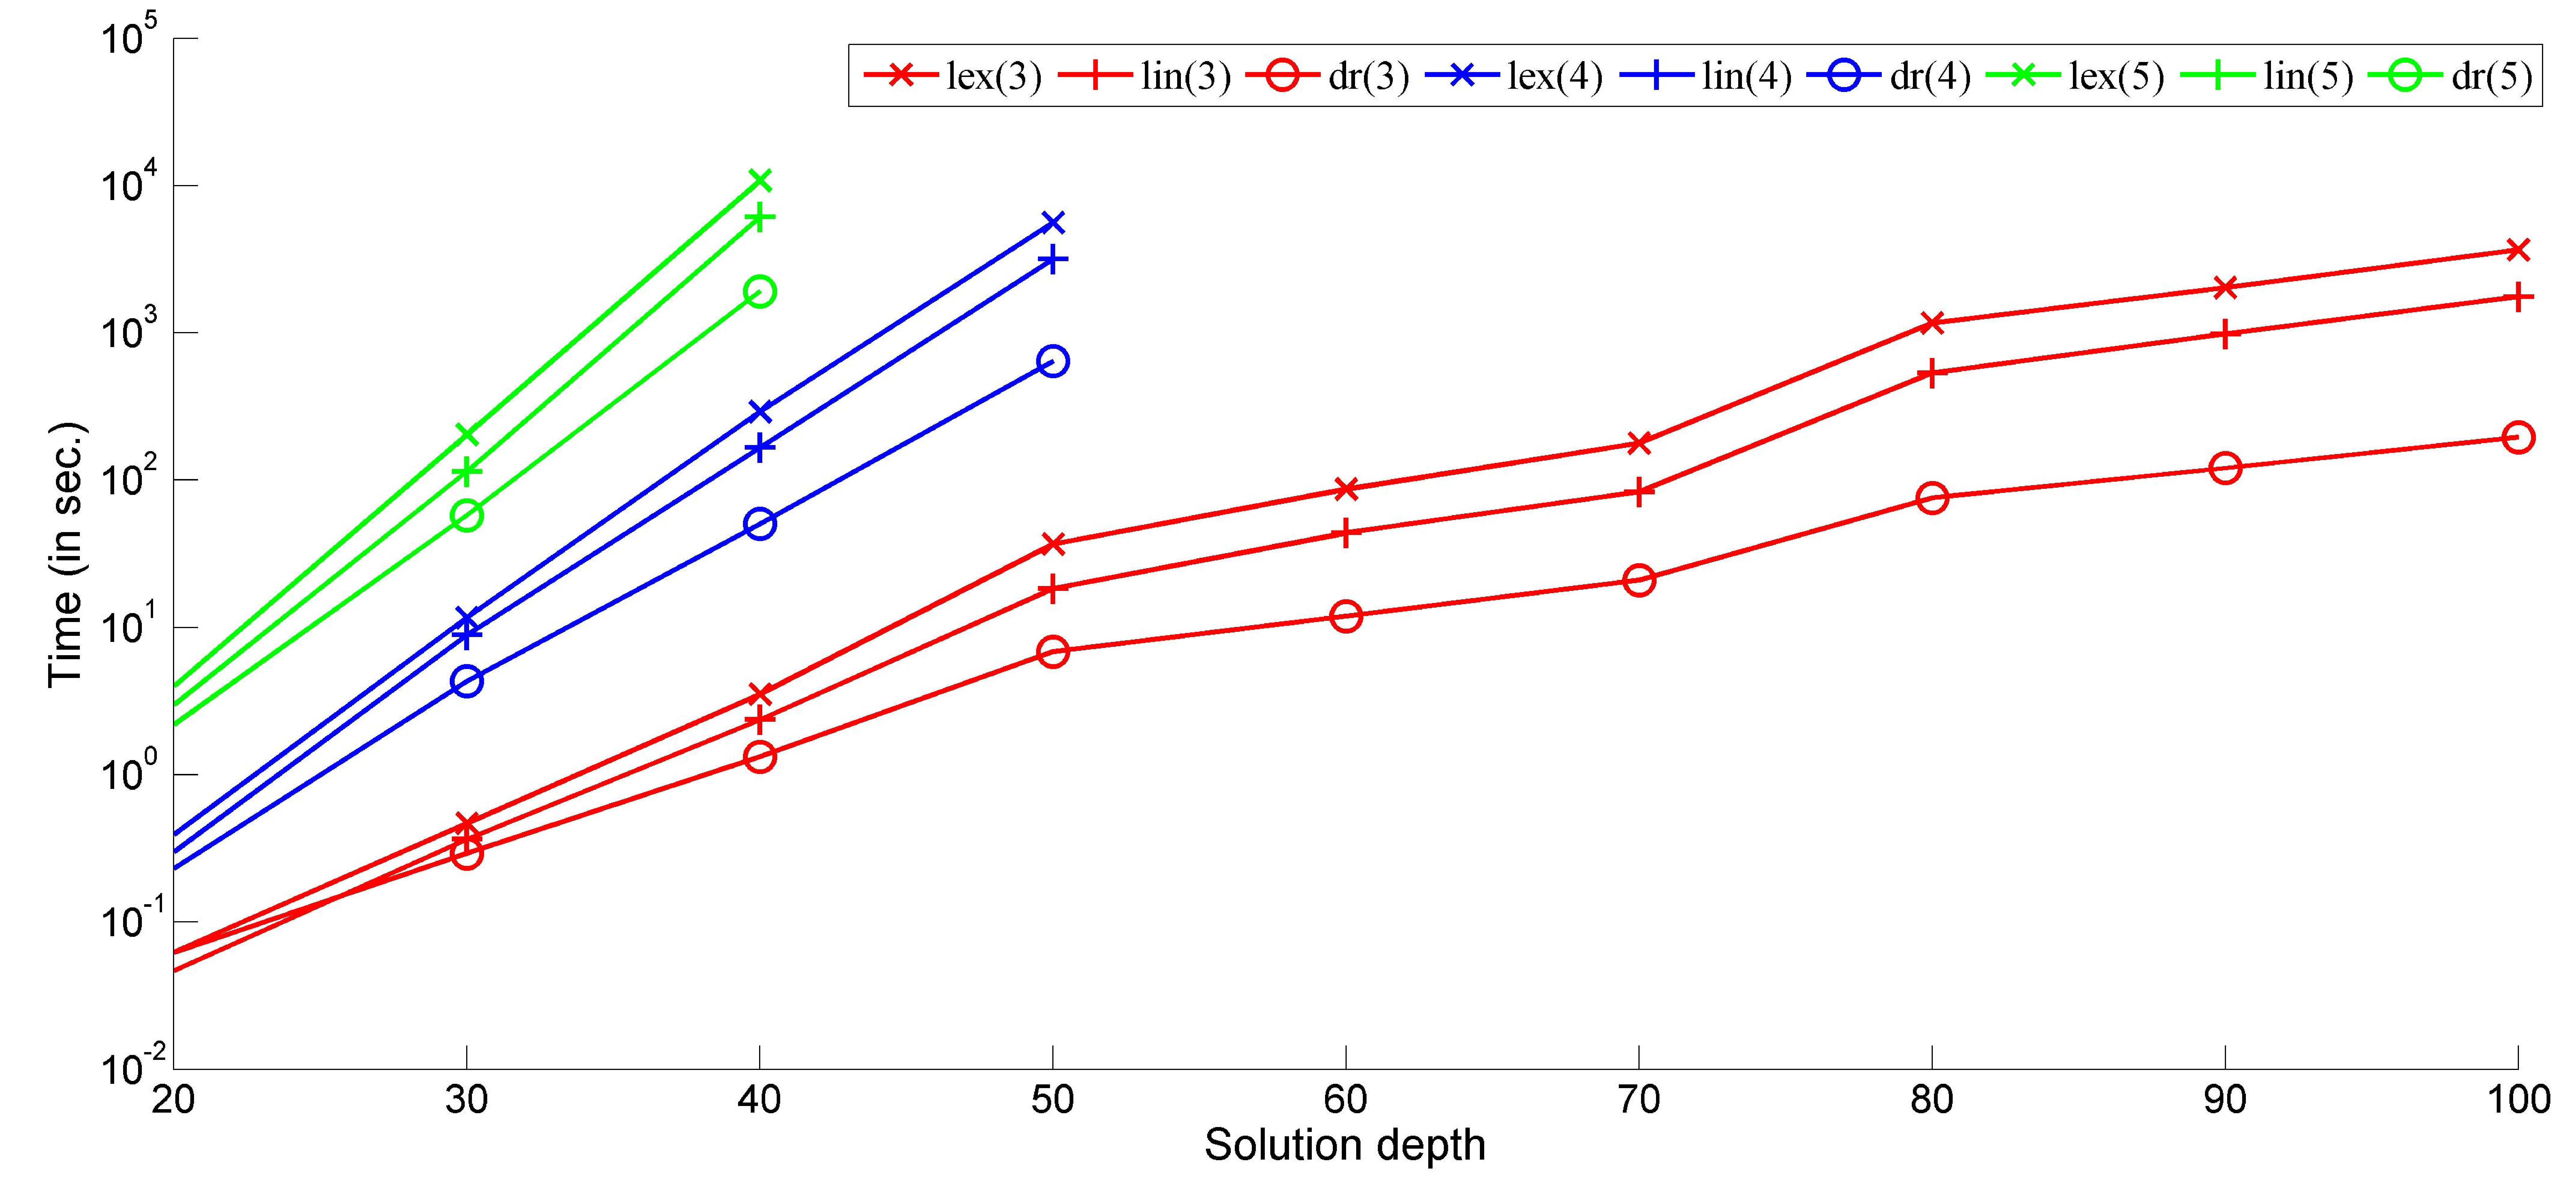
\includegraphics[width=1\textwidth]{Images/Chapter6/exe-time-grids-namoas}
\caption{Average runtimes for $q \in  \{3,4,5\}$ objectives per solution depth in grid problems.}
\label{fig:6-10}
\end{figure}

\begin{figure}%[ht]
\centering
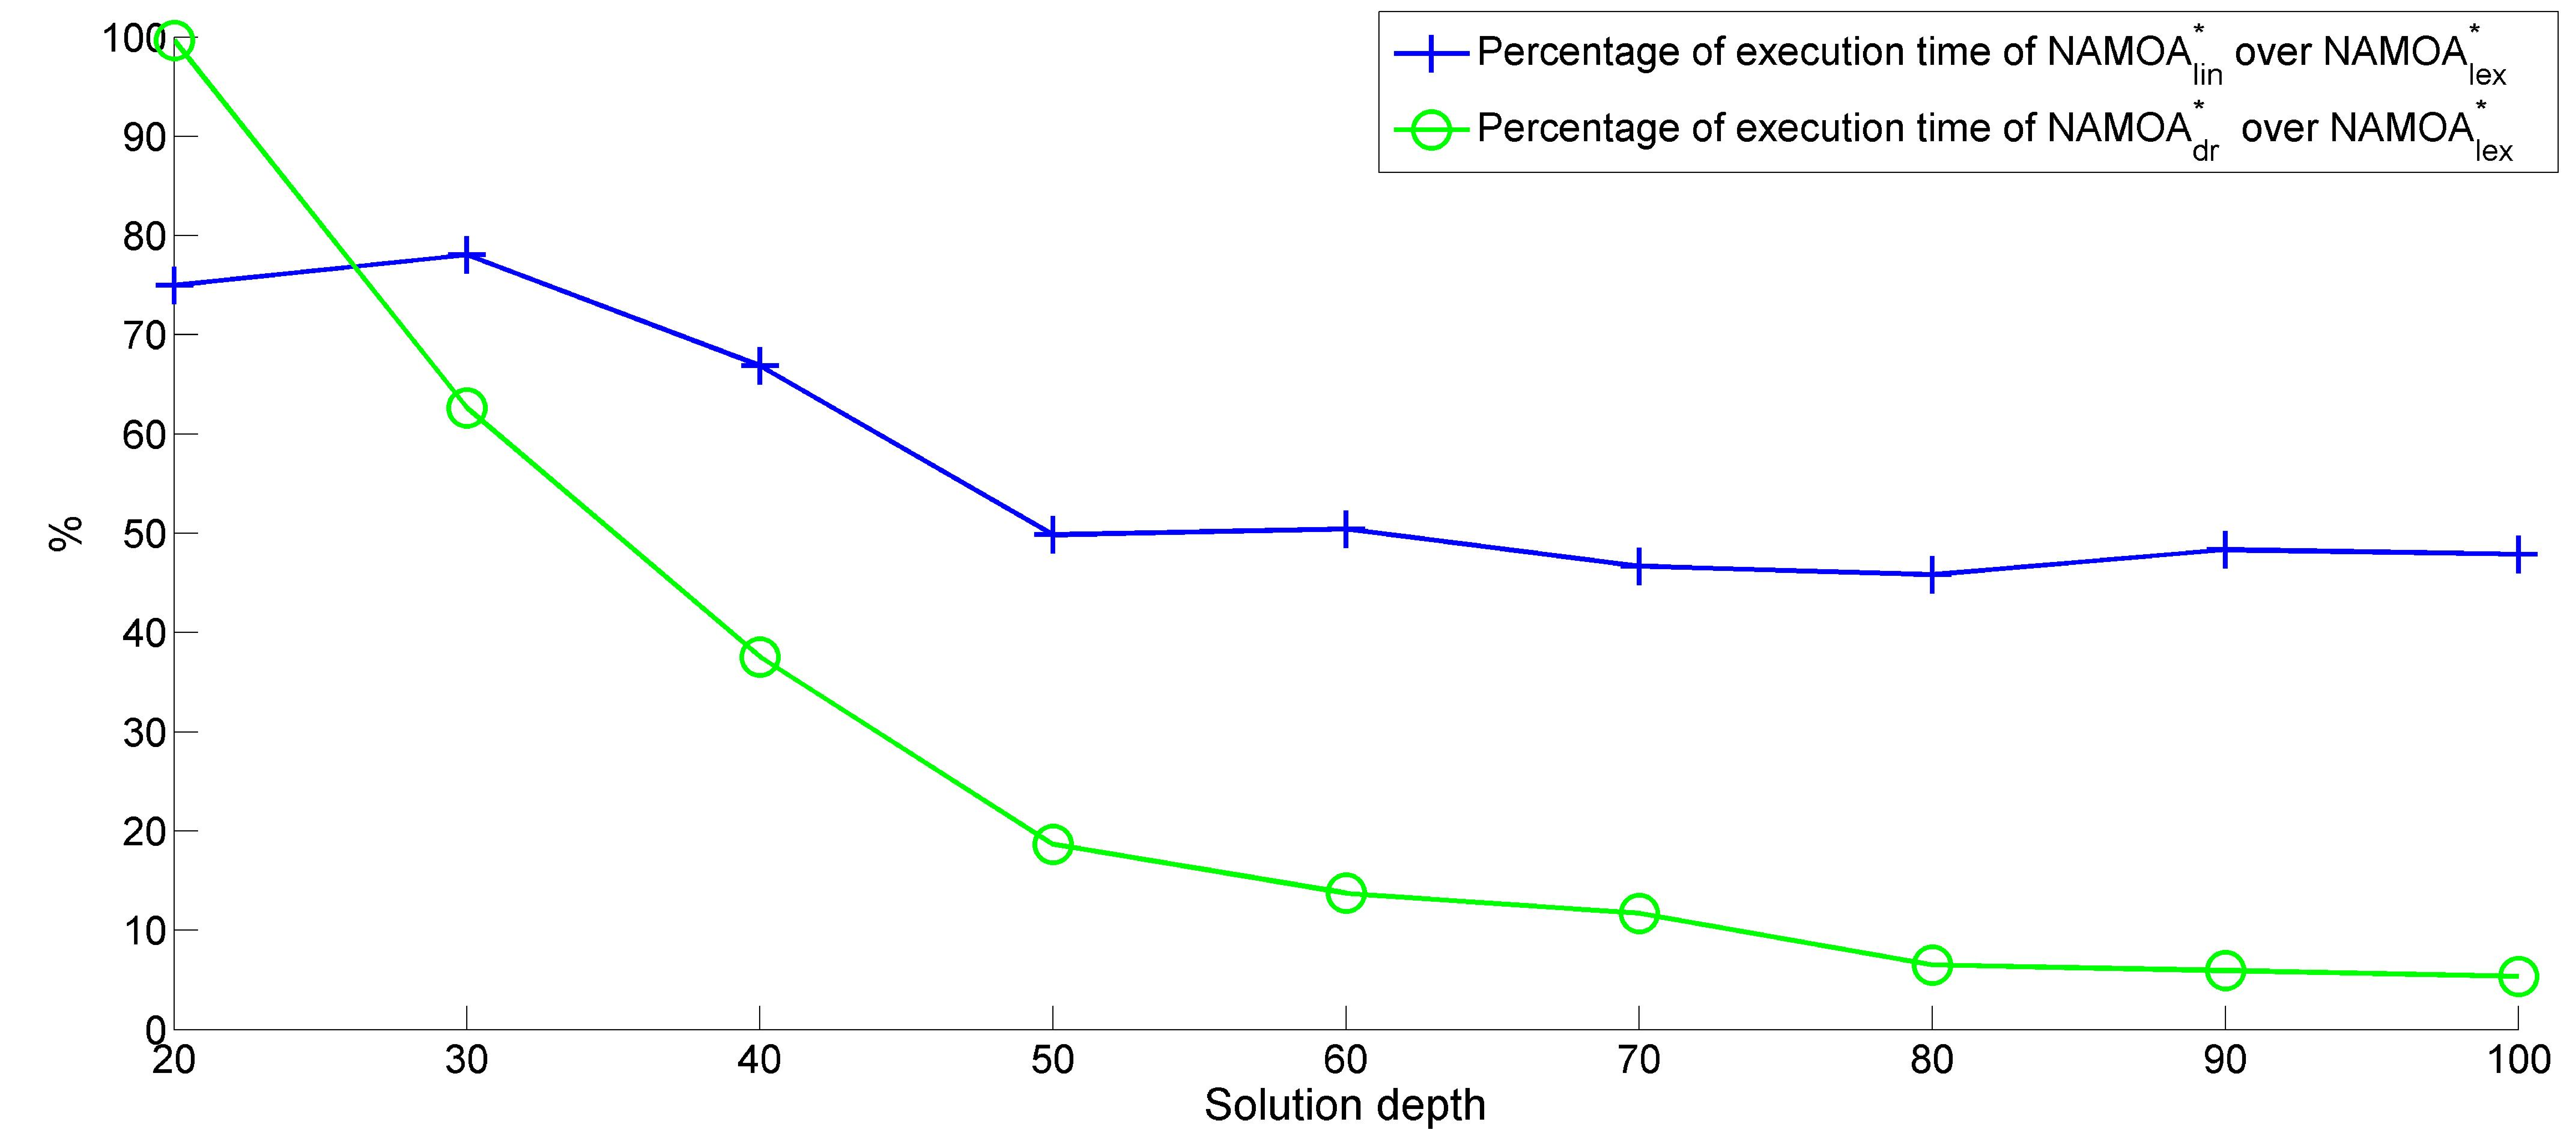
\includegraphics[width=1\textwidth]{Images/Chapter6/perc-exe-time-grids-namoas}
\caption{Percentage of average runtime of \namoate \ and \namoalin \ over \namoalex \ for $q = 3$ grid problems.}
\label{fig:6-11}
\end{figure}

%-------------------------------------------------------------------
\subsection{Summary}
\label{chapEmpiricalAnalysis:subsec:summarygridsnamoate}
%-------------------------------------------------------------------

A linear aggregation selection function is consistently more efficient in runtime than a lexicographic function when both are applied to standard \namoa. However, the lexicographic order can be exploited by the t-discarding technique for filtering and cl-pruning (\namoate). Results over grid problems reveal a dramatic improvement in runtime performance of over an order of magnitude for three-objective problems (see Figure \ref{fig:6-10}). The speedup of \namoate \ over \namoalex \ and \namoalin \ even grows with problem difficulty (see Table \ref{tab:6-7} and Figure \ref{fig:6-11}), reducing time requirements over 90\% for the harder $q = 3$ problems. When more objectives are considered, $q=\{4,5\}$, similar results can be observed, although a smaller number of experiments can be presented due to the increasing computational difficulty.  

As expected, multiobjective label-setting search spends most of the time performing dominance checks between labels. Every new label has to be checked for op-pruning, cl-pruning, and filtering. Figure \ref{fig:6-9} shows that, for the harder grid problems, cl-pruning is the operation that tends to discard most labels for deeper solutions. The same tendency can be observed regardless the number of objectives. 

While the ratio of labels discarded by filtering decreases with problem difficulty, it was always larger than the ratio of those discarded by op-pruning in our grid experiments. This is important for the efficiency of \namoate, since cl-pruning and filtering can both benefit from t-discarding. Table \ref{tab:6-6} reveals that the truncated sets of labels used by t-discarding are significantly smaller than the original ones, and their relative size even decreases with problem difficulty. For example, with solution depth $d = 100$ and $q = 3$, a label is checked against a set of 8,307 labels for filtering in the worst case with the standard procedure, while with t-discarding the worst case involves only a set of 137 labels (or 1.65\%). 

%-------------------------------------------------------------------
\section{\texorpdfstring{\lexgote}{LEXGO*dr} \ vs \texorpdfstring{\lexgo}{LEXGO*}}
\label{chapEmpiricalAnalysis:sec:resultsgridslexgote}
%-------------------------------------------------------------------

In this section we examine the performance of the dimensionality reduction technique applied to \lexgo, called \lexgote. A detailed description of \lexgo \ and \lexgote \ are presented in Section \ref{chapMultiObjAlg:subsec:lexgo} and Section \ref{chapMultiObjAlg:subsec:lexgote}, respectively. The experiments presented below are applied to the random grid problems with three objectives and goals defined in Section \ref{chapEmpiricalAnalysis:sec:grids}.

%-------------------------------------------------------------------
\subsection{Analysis on class I experiments}
\label{chapEmpiricalAnalysis:subsec:analysisgridslexgotec1}
%-------------------------------------------------------------------

Table \ref{tab:6-8} displays average runtimes for \lexgolex, \lexgolin, and \lexgote \ for depth $d = 100$. The last column shows the speed-up obtained by \lexgote \ over the best version of standard \lexgo \ for each value of $k_1$. \lexgote \ achieves important reductions in runtime when goals can be satisfied, i.e. when $k_1=\{1, 0.75, 0.5\}$ and it barely affects runtimes when goals cannot be satisfied, i.e. $k_1=\{0.25, 0\}$. Figure \ref{fig:6-12} shows graphically the relative runtime performance of \lexgote \ over the best previous runtimes of \lexgo, as a function of solution depth. Values corresponding to $k_1=0$ are not shown since they are practically zero. 

\begin{table}
\caption{Class I experiments on grids, average runtimes in seconds of \lexgolex, \lexgolin \ and \lexgote \ for $d = 100$. Speed-up of \lexgote \ over the best standard version of \lexgo.}
\centering
\begin{tabular}{rrrrr}
\cline{2-5} \noalign{\smallskip}
$k_1$ & \lexgolex & \lexgolin & \lexgote & Speedup\\
\noalign{\smallskip} \hline
1 & 3,763.78 & 2,114.18 & 254.40 & 8.31 \\
0.75 & 3,381.33 & 1,847.88 & 300.86 & 6.14\\
0.5 & 819.28 & 1,145.15 & 282.49 & 2.90 \\
0.25 & 33.47 & 37.45 & 35.37 & 0.94 \\
0 & 0.07 & 0.09 & 0.10 & 0.77\\
\hline
\end{tabular}
\label{tab:6-8}
\end{table}

\begin{figure}%[!ht]
\centering
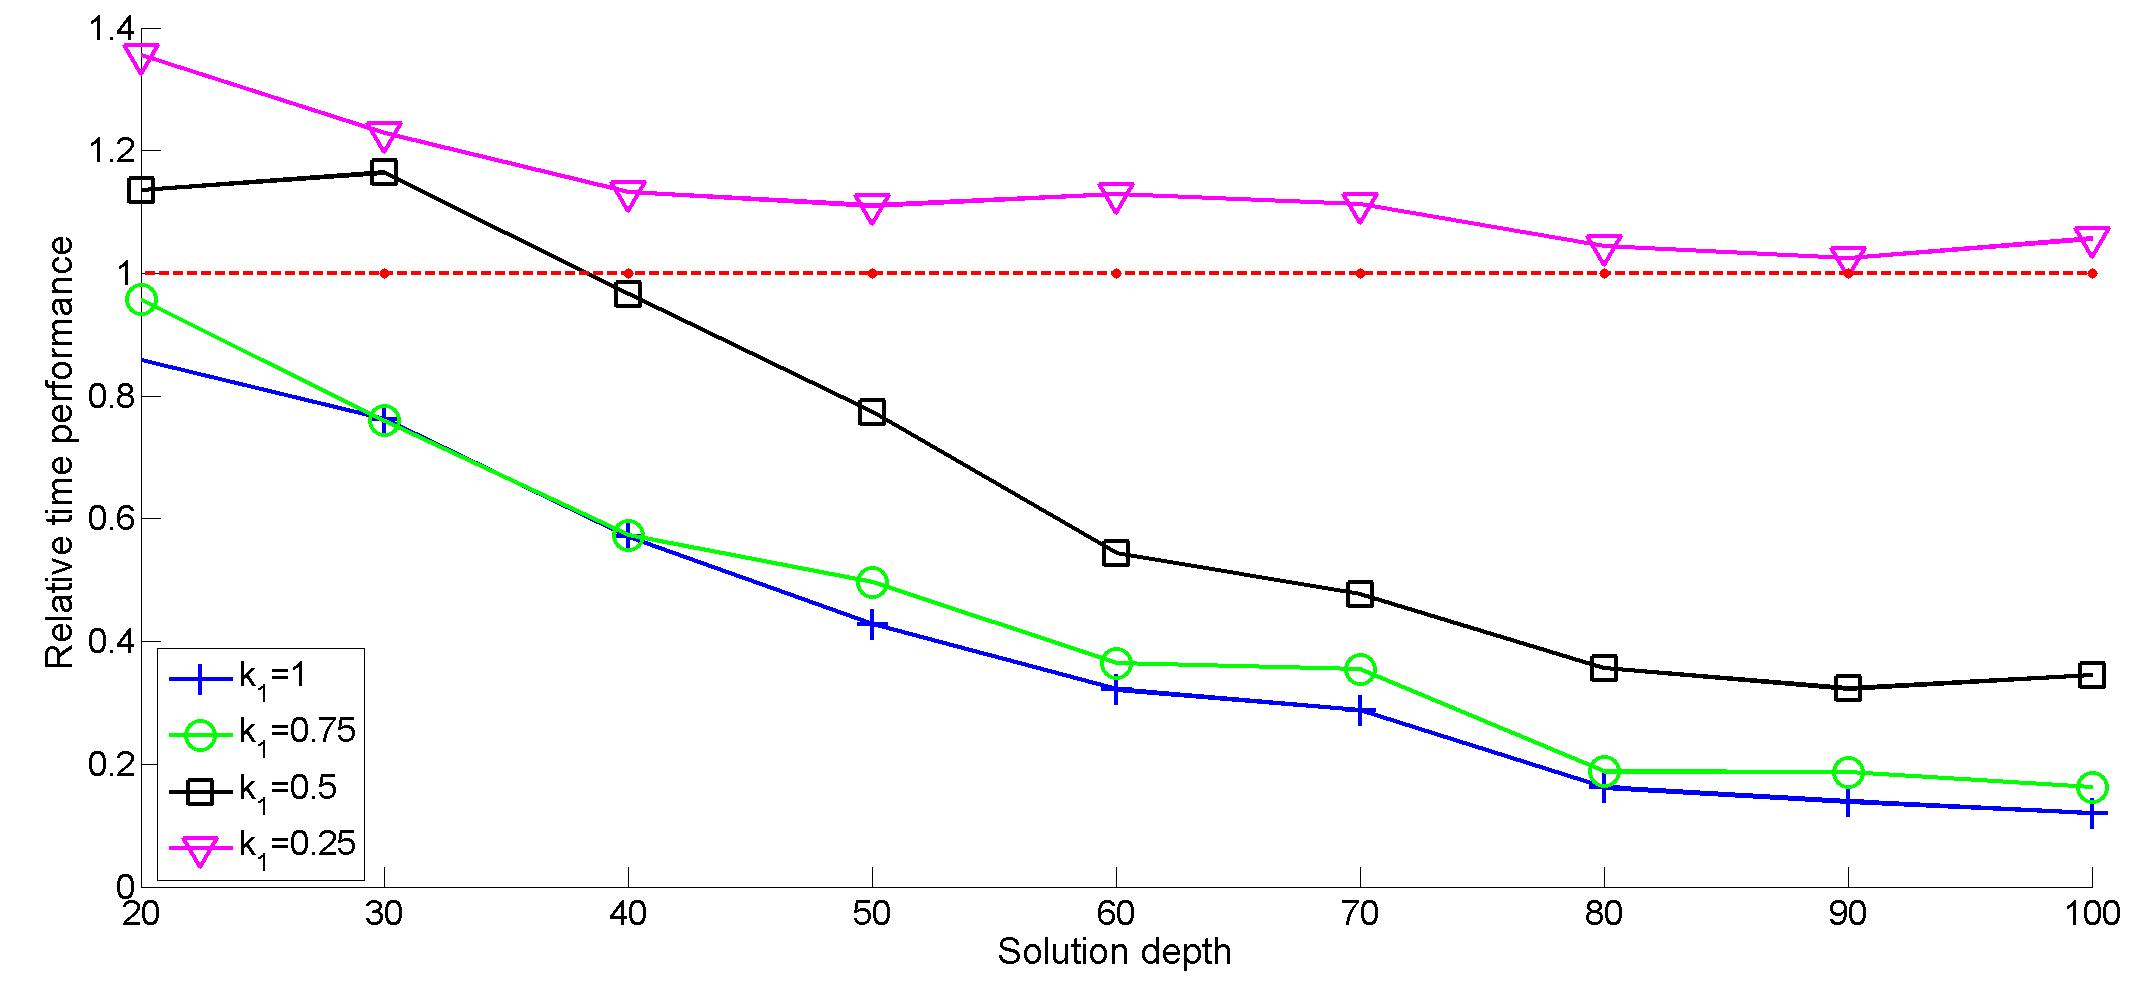
\includegraphics[width=1\textwidth]{Images/Chapter6/class1-exe-time-lexgo-te}
\caption{Class I experiments on grids, relative runtime performance of \lexgote \ over the best runtimes of standard \lexgo.}
\label{fig:6-12}
\end{figure}

%-------------------------------------------------------------------
\subsection{Analysis on class II experiments}
\label{chapEmpiricalAnalysis:subsec:analysisgridslexgotec2}
%-------------------------------------------------------------------

Table \ref{tab:6-9} shows the average runtimes of \lexgote \ for all possible values of $k_2$ with  $k_1=0.75$ and $k_1=0.5$. Figures \ref{fig:6-13a} and \ref{fig:6-13b} display, as a function of solution depth, the relative runtime performance of \lexgote \ over the best previous runtimes of \lexgo \ in $k_1=0.75$ and $k_1=0.5$, respectively.

Just as in the case of class I experiments, \lexgote \ obtains a better efficiency when the number of goal-optimal solution costs is greater. Thus, the relative runtime for $k_1=0.75$ is around 20\% and for $k_1=0.5$ around 30\% to 70\% of \lexgolin, the fastest version of the \lexgo \ algorithm so far. The sole case when \lexgote \ does not show improvement in practice is when  $k_1=0.5$ and  $k_2=0.125$. We can observe in Table \ref{tab:6-3} that in this case the goals are rarely satisfied by any problem instance.

\begin{table}
\caption{Class II experiments on grids, \lexgote \ runtimes in seconds.}
\centering
\begin{tabular}{rrrrrrrrrr}
\hline \noalign{\smallskip}
 & \multicolumn{8}{c}{\lexgote} & \\
\noalign{\smallskip} \cline{2-9}
 & \multicolumn{4}{c|}{0.75} & \multicolumn{4}{c}{0.5} & \multicolumn{1}{c}{$k_1$}\\
\multicolumn{1}{c}{$d$} & 0.75 & 0.5625 & 0.375 & \multicolumn{1}{c|}{0.1875} & 0.5 & 0.375 & 0.25 & 0.125 & \multicolumn{1}{c}{$k_2$}\\
\cline{1-9} \noalign{\smallskip} 
\multicolumn{1}{c}{20} & 0.07 & 0.06 & 0.04 & 0.01 & 0.03 & 0.02 & 0.01 & <0.01 \\ 
\multicolumn{1}{c}{30} & 0.38 & 0.35 & 0.23 & 0.09 & 0.22 & 0.15 & 0.08 & 0.05 \\ 
\multicolumn{1}{c}{40} & 1.7 & 1.6 & 1.1 & 0.38 & 1.1 & 0.81 & 0.42 & 0.24 &  \\ 
\multicolumn{1}{c}{50} & 10.3 & 10.6 & 6.5 & 1.7 & 6.5 & 4.2 & 1.9 & 0.84 \\ 
\multicolumn{1}{c}{60} & 17.3 & 19.3 & 13.5 & 3.6 & 14.4 & 10.3 & 4.8 & 1.8 \\  
\multicolumn{1}{c}{70} & 30.8 & 32.2 & 22.8 & 6.8 & 24.0 & 17.7 & 8.5 & 2.9 \\
\multicolumn{1}{c}{80} & 105.9 & 133.1 & 95.0 & 24.0 & 97.8 & 68.5 & 29.4 & 17.4 \\ 
\multicolumn{1}{c}{90} & 187.9 & 219.8 & 156.5 & 41.2 & 158.7 & 117.8 & 53.3 & 40.0 \\ 
\multicolumn{1}{c}{100} & 300.8 & 389.6 & 283.7 & 63.4 & 282.4 & 199.1 & 84.7 & 82.1 \\ 
\hline
\end{tabular}
\label{tab:6-9}
\end{table} 

\begin{figure}
    \begin{center}
%
      \subfigure[$k_1 = 0.75$]{%
         \label{fig:6-13a}
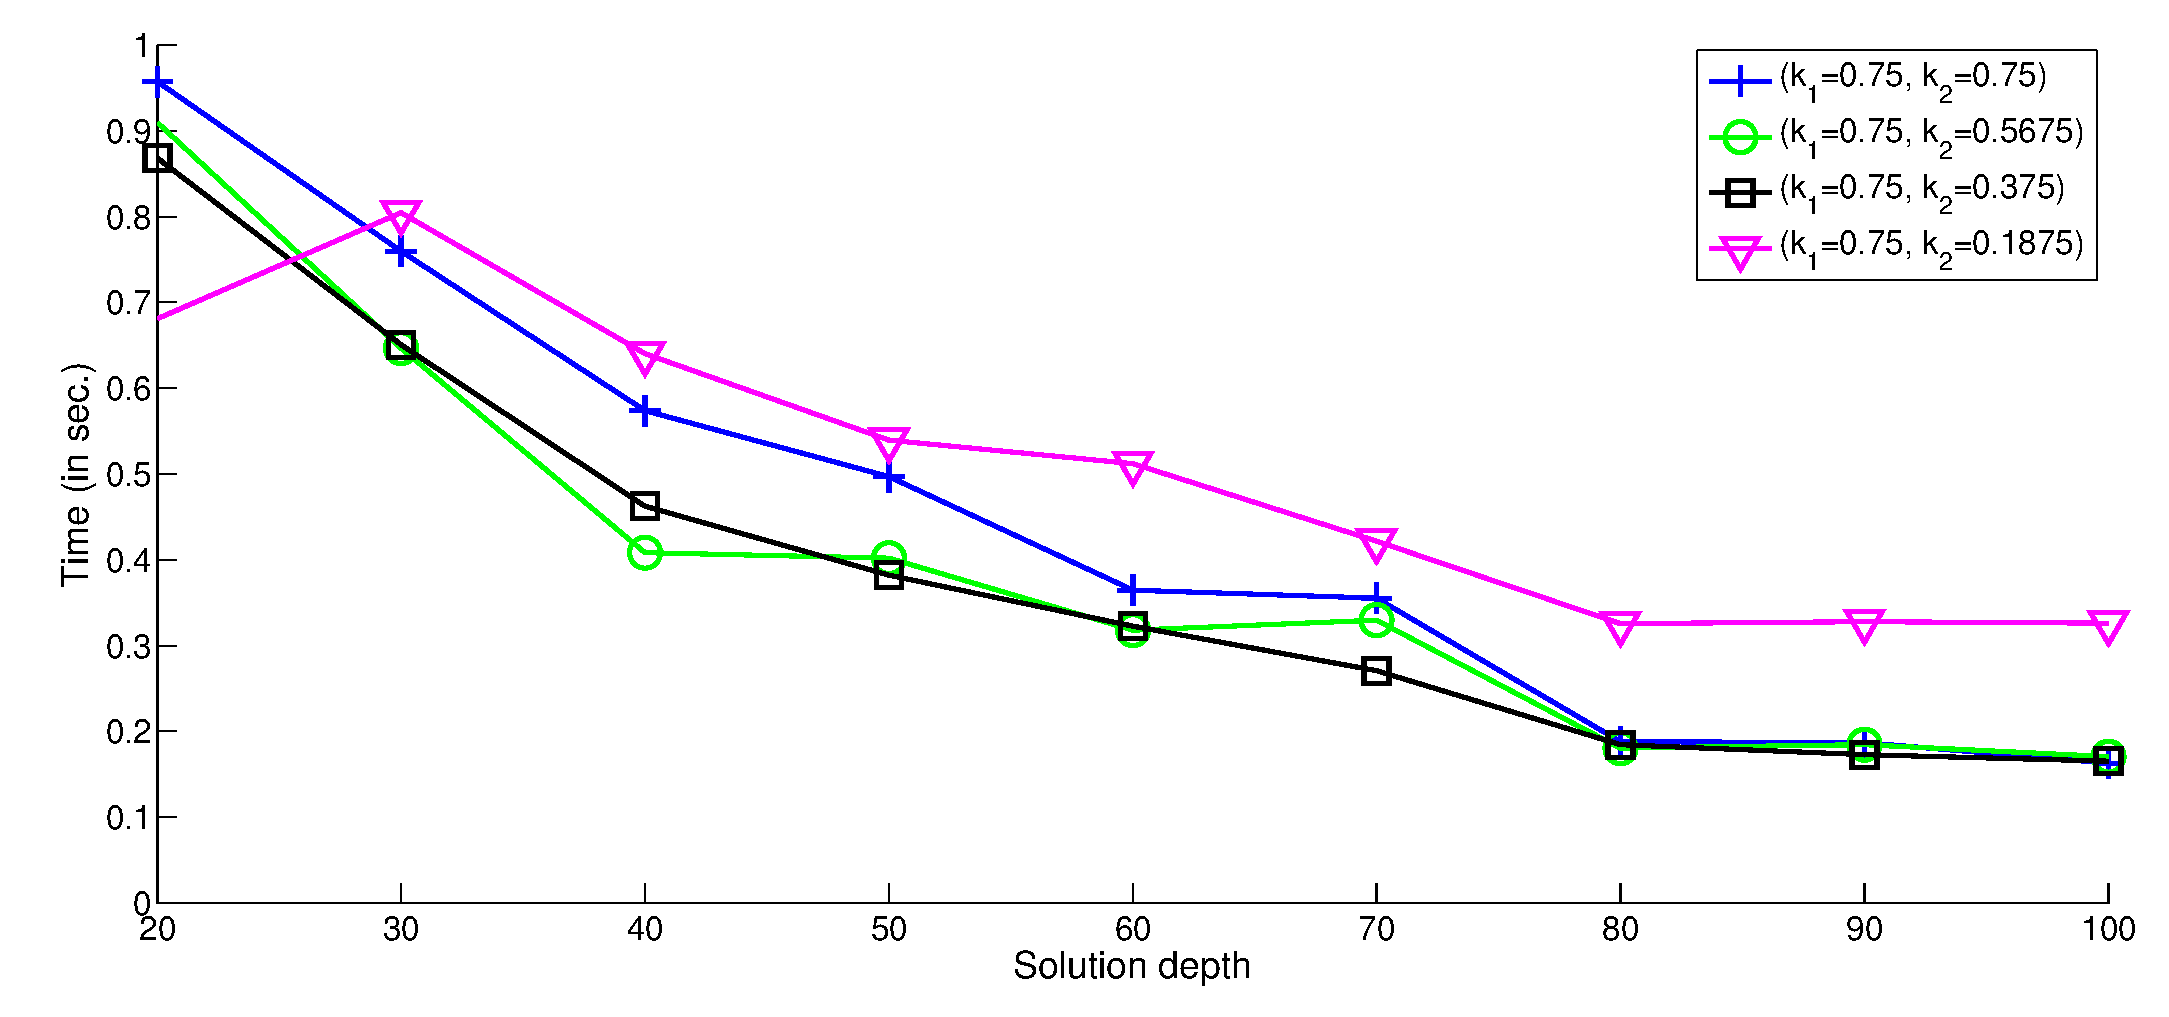
\includegraphics[width=0.95\textwidth]{Images/Chapter6/class2-exe-time-lexgo-te-a}
        }\\ %  ------- End of the first row ----------------------%
\vspace{0.025\textwidth}      
		\subfigure[$k_1 = 0.5$]{%
         \label{fig:6-13b}  
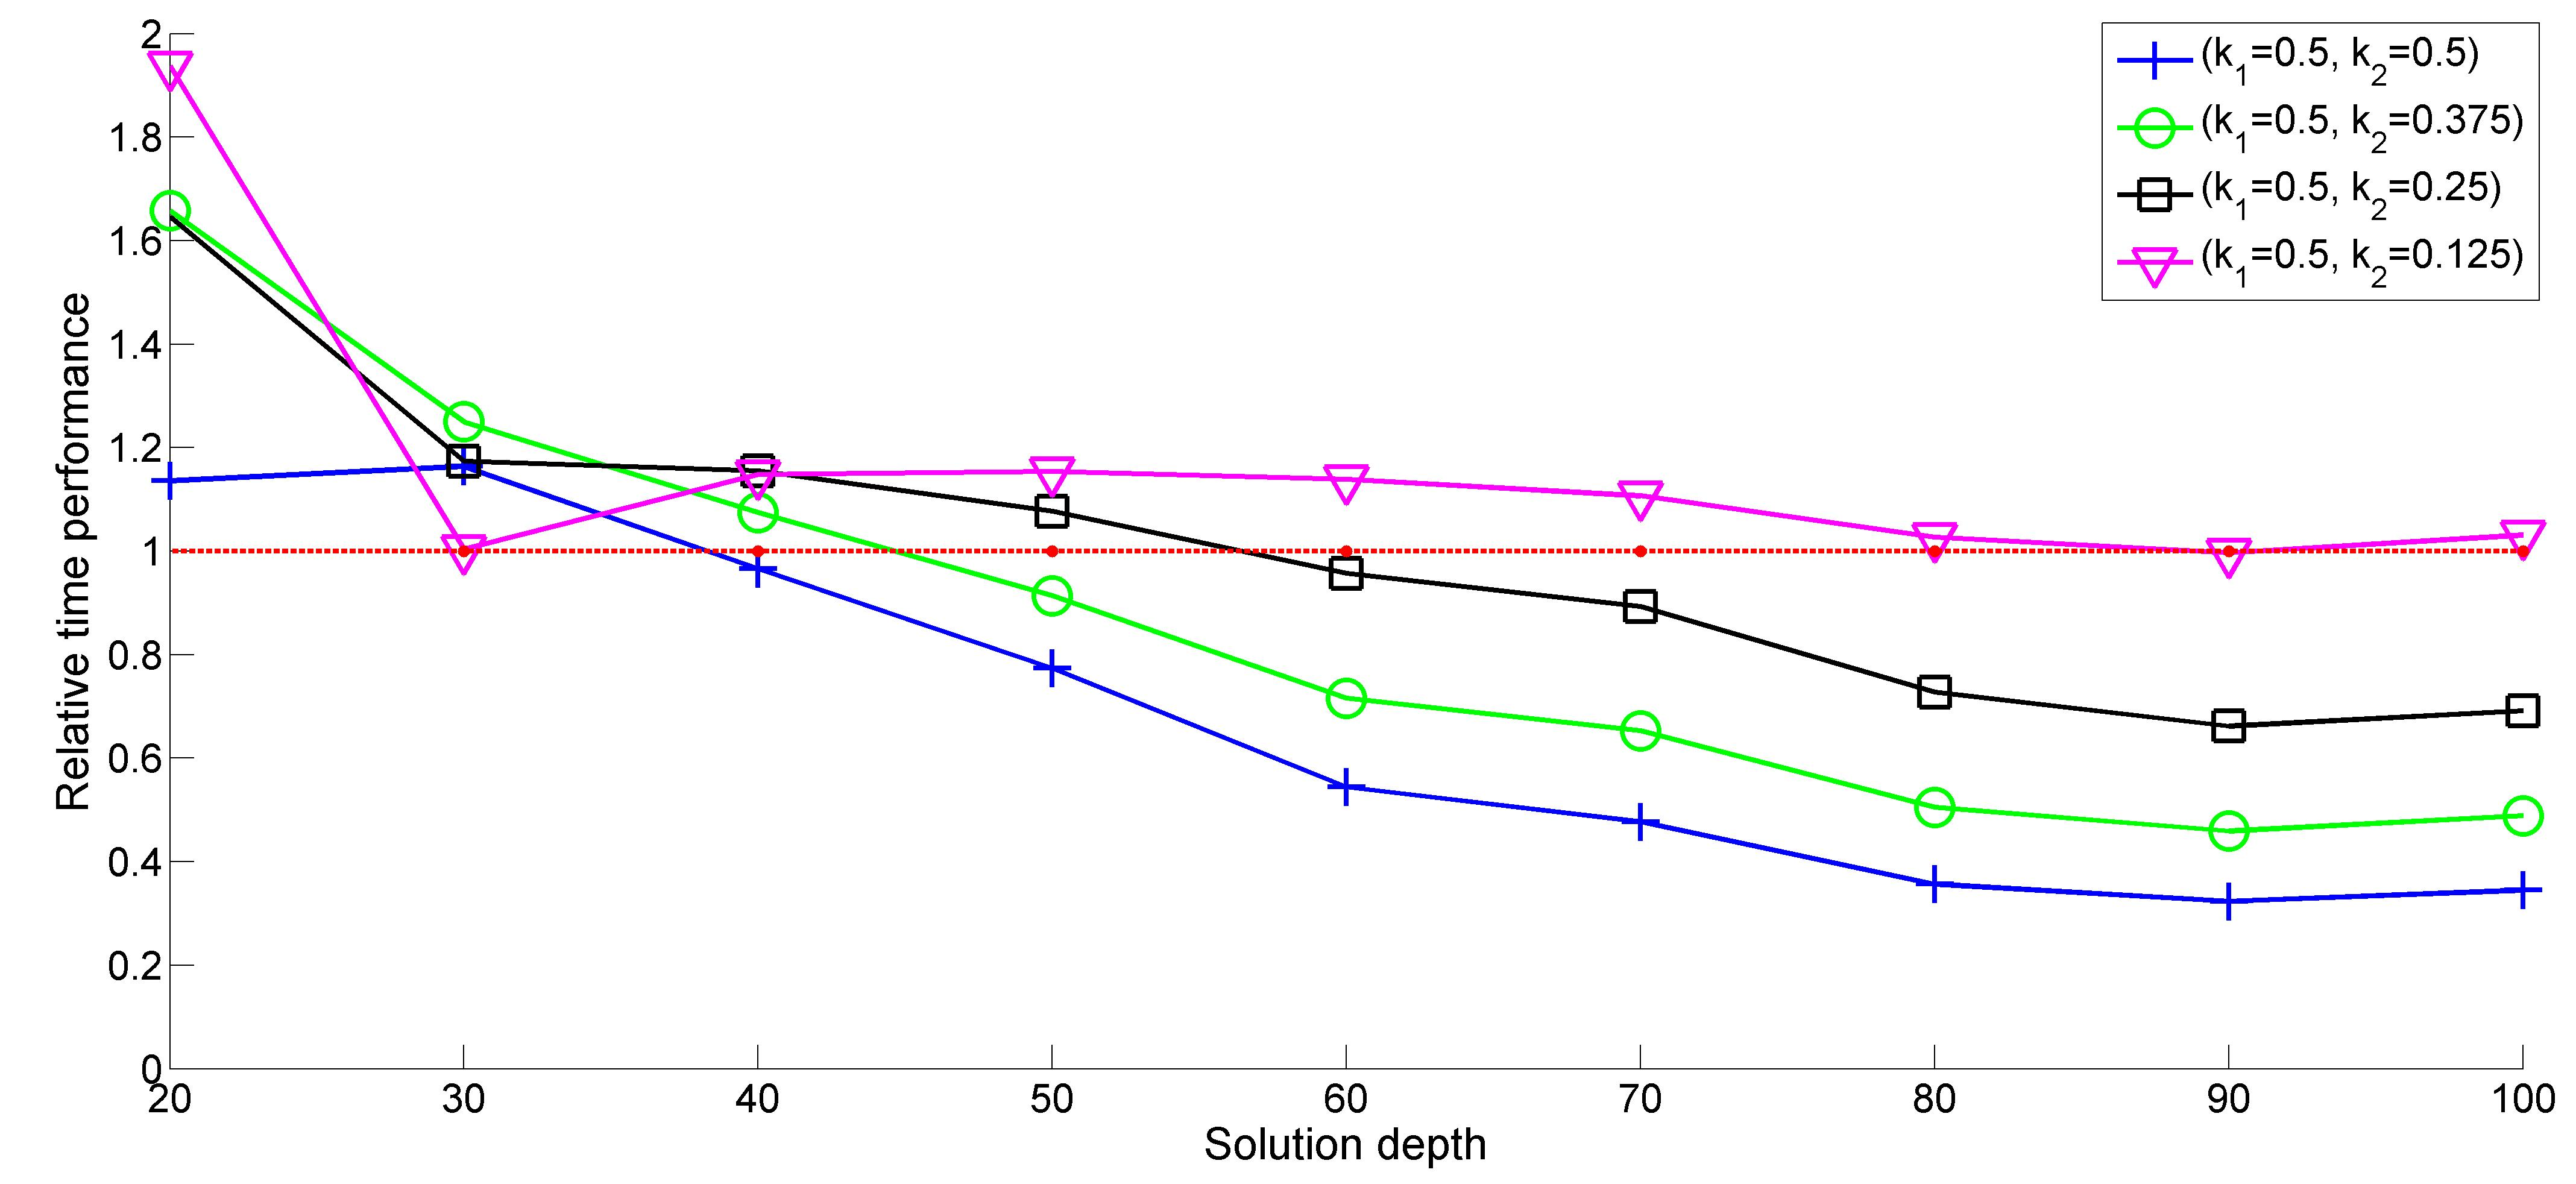
\includegraphics[width=0.95\textwidth]{Images/Chapter6/class2-exe-time-lexgo-te-b}
        }\\ %  ------- End of the first row ----------------------%
    \end{center}
    \vspace{-0.25in} 
    \caption{%
Class II experiments on grids, relative runtime performance (in seconds) of \lexgote \ over the best previous runtimes of \lexgo \ as a function of solution depth.
    }%
    \label{fig:6-13}
\end{figure}

%-------------------------------------------------------------------
\subsection{Summary}
\label{chapEmpiricalAnalysis:subsec:summarygridslexgote}
%-------------------------------------------------------------------

Just as in the case of \namoa, \lexgo \ can also be improved when applying the t-discarding method. This method can be applied to \lexgo \ when goals can be satisfied, i.e. when deviation vectors are $\vec 0$.

In a similar way as \namoate \ performs against \namoa \ (see Section \ref{chapEmpiricalAnalysis:sec:resultsgridsnamoate}), the speed-up of \lexgote \ over \lexgo \ grows with problem difficulty (see Figures \ref{fig:6-12},  and \ref{fig:6-13}), reducing time requirements over 88\% for the harder problems. In addition, \lexgote \ speed-up grows with the number of goal-optimal solution costs. Notice in Table \ref{tab:6-8} that \lexgote \ for $d=100$ runs 11\% faster with $k_1= 1$ than with $k_1=0.5$, despite of the fact that the number of label expansions is 40\% greater for $k_1=1$ than for $k_1=0.5$ (see Tables \ref{tab:6-2a} and \ref{tab:6-2b}). This is because the number of opportunities to apply t-discarding grows with the relative percentage of goal-optimal solution costs over the Pareto set. Hence, t-discarding is triggered on a more regular basis on these cases where $k_1$ is greater.

\lexgote \ does not show any improvement when goals cannot be satisfied, since the t-discarding can be barely applied to these problems. However, \lexgo \ achieves important reductions in time when goals can be satisfied, being three to eight times faster in class I experiments and up to six times faster in the second class of experiments.

%-------------------------------------------------------------------
\section{\texorpdfstring{\lexgote}{LEXGO*dr} \ vs \texorpdfstring{\namoate}{NAMOA*dr}}
\label{chapEmpiricalAnalysis:sec:resultsgridsfinal}
%-------------------------------------------------------------------

This section deals with the algorithms that employ the dimensionality reduction technique, \namoate \ and \lexgote. We have already seen the improvement of \namoate \ over \namoa, as well as \lexgote \ over \lexgo. In the following, a final time performance comparison between the two best alternatives is presented.

The experiments included in this section are applied to random grid problems with three objectives and goals described in Section \ref{chapEmpiricalAnalysis:sec:grids}.

%-------------------------------------------------------------------
\subsection{Analysis on class I experiments}
\label{chapEmpiricalAnalysis:subsec:analysisgridsfinalc1}
%-------------------------------------------------------------------

Table \ref{tab:6-10} shows the relative performance of \lexgote \ over \namoate \ for the solution depth equal to 100. \lexgote \ performs better than \namoate \ when goals cannot be satisfied, i.e. $k_1=\{0.25, 0\}$ but it is significantly slower when goals can be satisfied. It is also worth to pay attention to the relative performance when $k_1=1$ in comparison with $k_1=0.5$. The former performs around 40\% more label expansions (see Table \ref{tab:6-2}) and it is still faster than the latter. Notice that the number of scanned labels of both algorithms that employ the dimensionality reduction technique are equal to their versions without t-discarding, although the number of dominance checks is greatly reduced in \namoate \ and \lexgote.

Figure \ref{fig:6-14} displays the average runtimes of \namoate \ and \lexgote \ as a function of solution depth. The trend here is slightly in favor of \namoate \ over \lexgote \ for $k_1 \geq 0.5$.

\begin{table}
\caption{Class I experiments on grids, runtimes of \lexgote \ and \namoate \ for $d = 100$.}
\centering
\begin{tabular}{rrrrrr}
\hline \noalign{\smallskip}
 & \multicolumn{5}{c}{\lexgote} \\
\noalign{\smallskip} \cline{2-6} \noalign{\smallskip}
\namoate & $(k_1=1)$ & $(k_1=0.75)$ & $(k_1=0.5)$ & $(k_1=0.25)$ & $(k_1=0)$ \\
\noalign{\smallskip} 
Runtime (s) \\
\hline  \noalign{\smallskip} 
196.1 & 254.4 & 300.8 & 282.5 & 35.3 & 0.1 \\ 
%\hline
%\% & \% & \% & \% & \% & \% \\
%100\% & 129.7\% & 153.4\% & 144\% & 18\% & 0.04\% \\
\hline
\end{tabular}
\label{tab:6-10}
\end{table} 

\begin{figure}%[!ht]
\centering
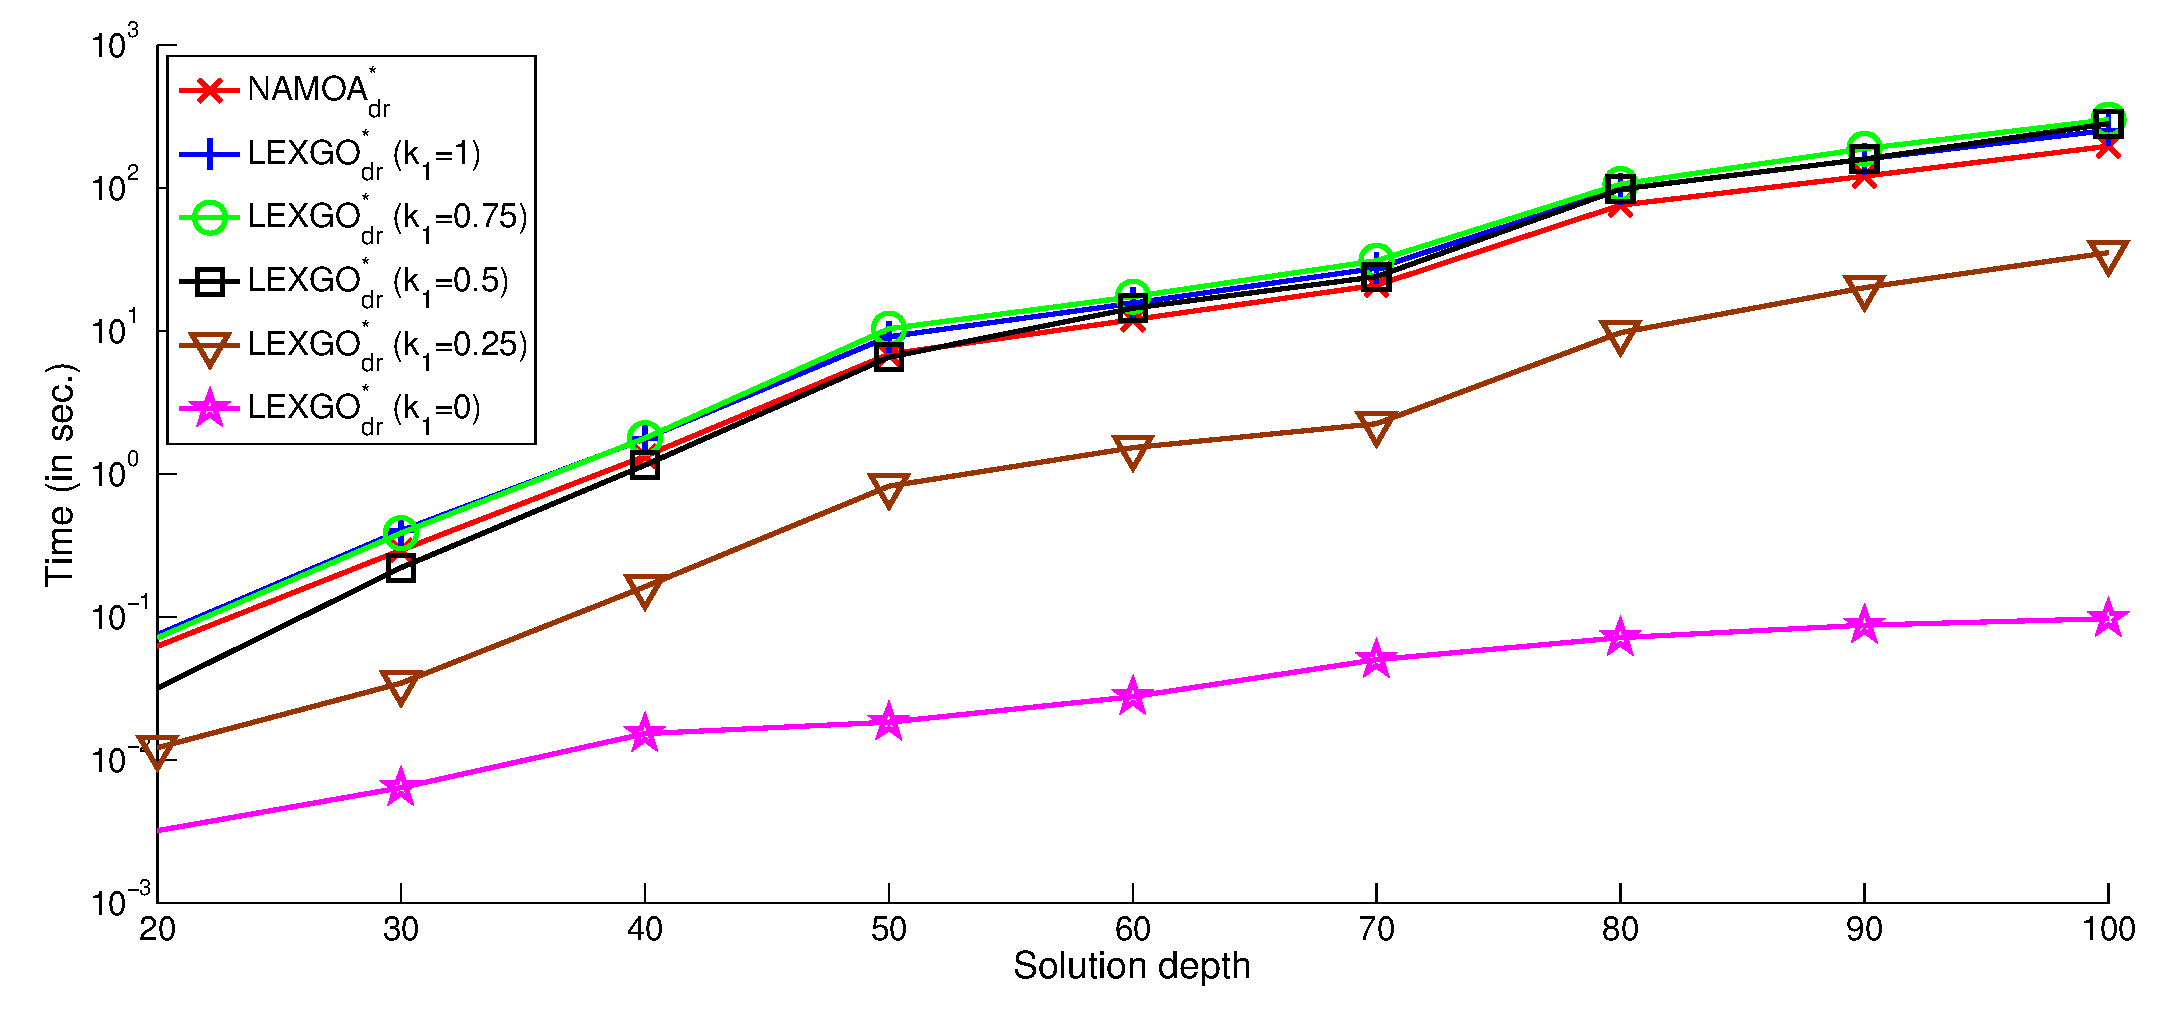
\includegraphics[width=1\textwidth]{Images/Chapter6/class1-exe-time-te}
\caption{Class I experiments on grids, average runtimes (in seconds) of \namoate \ and \lexgote \ per solution depth.}
\label{fig:6-14}
\end{figure}

%-------------------------------------------------------------------
\subsection{Analysis on class II experiments}
\label{chapEmpiricalAnalysis:subsec:analysisgridsfinalc2}
%-------------------------------------------------------------------

Regarding the second class of experiments, Table \ref{tab:6-11} shows \namoate \ and \lexgote \ runtimes for $k_1=0.75$ and $k_1=0.5$ with all $k_2$ possible values. Those cases where \lexgote \ outperforms \namoate \ are shown in bold. Figures \ref{fig:6-15a} and \ref{fig:6-15b} display the runtimes as a function of solution depth for $k_1=0.75$ and $k_1=0.5$, respectively. 

In these experiments, it can be observed that there are cases when goals are satisfiable and \lexgote \ is still faster than \namoate. On one hand, when $k_1=0.75, k_2=0.1875$ approximately 10\% of the Pareto frontier is returned (see Table \ref{tab:6-3}) and \lexgote \ is somewhat three times faster than \namoate. On the other hand, when $k_1=0.5$ and $k_2=0.25$ goals can also be satisfied and \lexgote \ outperforms \namoate. 

\begin{table}
\caption{Class II experiments on grids, \lexgote \ and \namoate \ runtimes (in seconds). Cases were \lexgote \ outperforms \namoate \ are highlighted in bold.}
\centering
\scalebox{0.9}{
\begin{tabular}{rrrrrrrrrrr}
\hline \noalign{\smallskip}
 &  & \multicolumn{8}{c}{\lexgote} & \\
\noalign{\smallskip} \cline{3-10}
 & \namoate & \multicolumn{4}{c|}{0.75} & \multicolumn{4}{c}{0.5} & \multicolumn{1}{c}{$k_1$}\\
$d$  & Runtime (s) & 0.75 & 0.5625 & 0.375 & \multicolumn{1}{c|}{0.1875} & 0.5 & 0.375 & 0.25 & 0.125 & \multicolumn{1}{c}{$k_2$}\\
\cline{1-10} \noalign{\smallskip} 
20 & 0.06 & 0.07 & \textbf{0.06} & \textbf{0.04} & \textbf{0.01} & \textbf{0.03} & \textbf{0.02} & \textbf{0.01} & \textbf{<0.01} \\ 
30 & 0.29 & 0.38 & 0.35 & \textbf{0.23} & \textbf{0.09} & \textbf{0.22} & \textbf{0.15} & \textbf{0.08} & \textbf{0.05} \\ 
40 & 1.3 & 1.7 & 1.6 & \textbf{1.1} & \textbf{0.38} & \textbf{1.1} & \textbf{0.81} & \textbf{0.42} & \textbf{0.24} \\ 
50 & 6.8 & 10.3 & 10.6 & \textbf{6.5} & \textbf{1.74} & \textbf{6.5} & \textbf{4.2} & \textbf{1.9} & \textbf{0.84} \\ 
60 & 11.9 & 17.3 & 19.3 & 13.5 & \textbf{3.6} & 14.4 & \textbf{10.4} & \textbf{4.8} & \textbf{1.8} \\  
70 & 20.9 & 30.8 & 32.2 & 22.8 & \textbf{6.8} & 24.0 & \textbf{17.7} & \textbf{8.5} & \textbf{2.9} \\
80 & 76.0 & 105.9 & 133.1 & 95.0 & \textbf{24.0} & 97.8 & \textbf{68.5} & \textbf{29.4} & \textbf{17.4} \\ 
90 & 120.6 & 187.9 & 219.8 & 156.5 & \textbf{41.2} & 158.7 & \textbf{117.8} & \textbf{53.3} & \textbf{40.0} \\ 
100 & 196.1 & 300.8 & 389.6 & 283.7 & \textbf{63.4} & 282.4 & 199.1 & \textbf{84.7} & \textbf{82.1} \\ 
\hline
\end{tabular}
}
\label{tab:6-11}
\end{table} 

\begin{figure}
    \begin{center}
%
      \subfigure[$k_1 = 0.75$]{%
         \label{fig:6-15a}
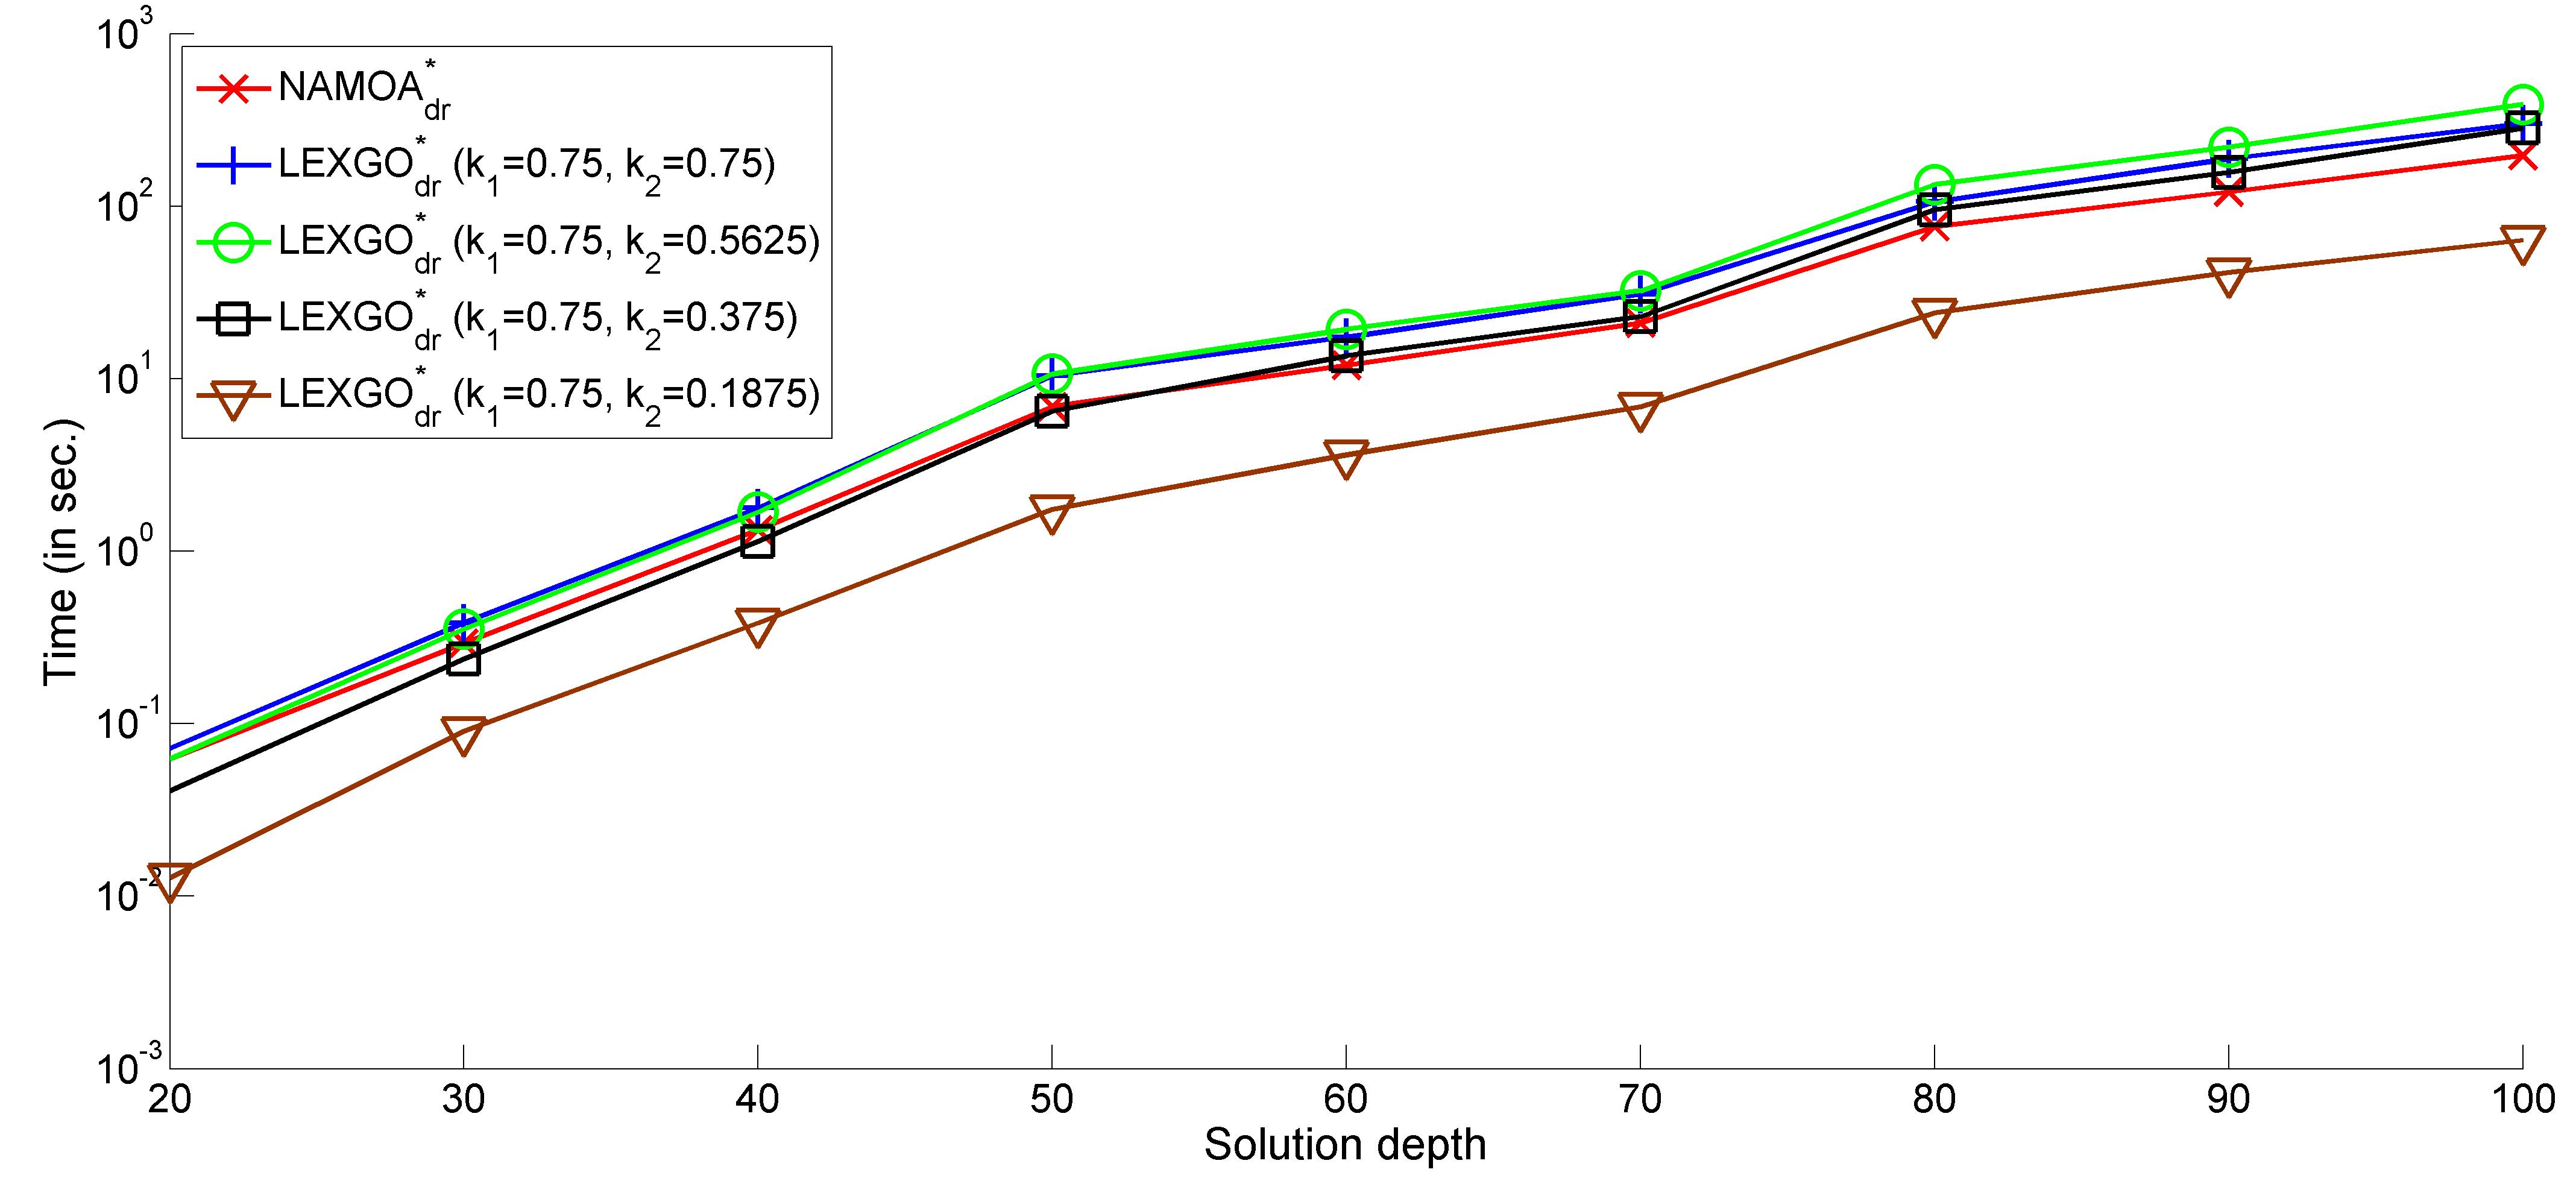
\includegraphics[width=0.95\textwidth]{Images/Chapter6/class2-exe-time-te-a}
        }\\ %  ------- End of the first row ----------------------%
\vspace{0.025\textwidth}      
		\subfigure[$k_1 = 0.5$]{%
         \label{fig:6-15b}  
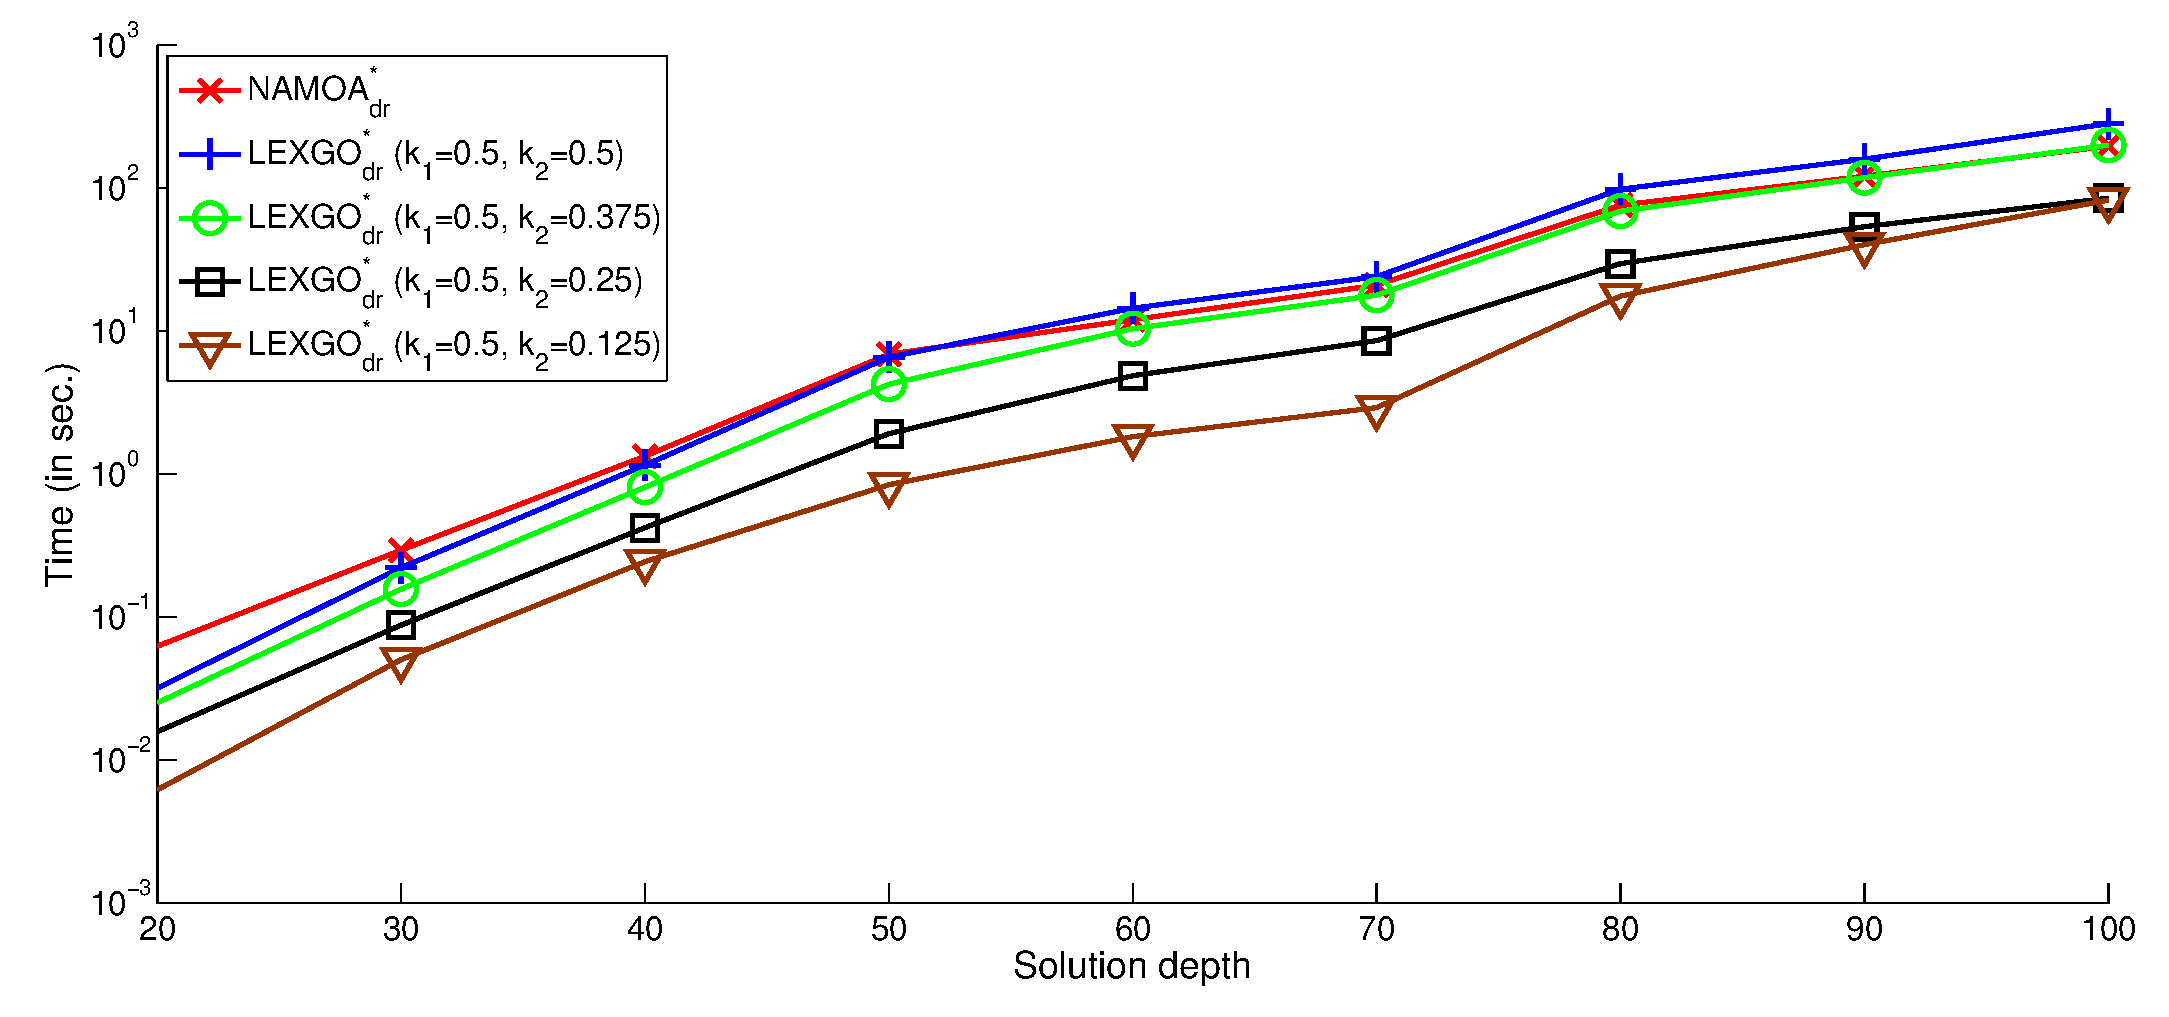
\includegraphics[width=0.95\textwidth]{Images/Chapter6/class2-exe-time-te-b}
        }\\ %  ------- End of the first row ----------------------%
    \end{center}
    \vspace{-0.25in} 
    \caption{%
Class II experiments on grids, average runtimes in seconds of \lexgote \ and \namoate \ per solution depth.
    }%
    \label{fig:6-15}
\end{figure}

%-------------------------------------------------------------------
\subsection{Summary}
\label{chapEmpiricalAnalysis:subsec:summarygridste}
%-------------------------------------------------------------------

The experimental comparison between \namoate \ and \lexgote \ is one of the contributions of this thesis. On one hand, \lexgote \ is the application of the successful technique of t-discarding dominated paths to the algorithm \lexgo, which has also been proposed in this thesis. In fact, these results are new to the literature and expose a significant different behavior than the comparison between \lexgo \ and \namoa \ showed in Section \ref{chapEmpiricalAnalysis:sec:resultsgridslexgo}. Despite \lexgo \ has been proved to be more efficient than \namoa \ (see Section \ref{chapFormalAnalysis:sec:efficiencyLexgo}), the same cannot be asserted when the t-discarding technique is applied to both algorithms. 

Both \namoate \ and \lexgote \ achieve a speed-up of about an order of magnitude for our random grid problem experiments over \namoa \ and \lexgo, respectively. However, \lexgote \ cannot apply the t-discarding method when a path does not satisfy goals and therefore, the applicability of this technique is partial, even though practically is applied to an average of 99.5\% of the pruning operations. This small percentage of iterations that must perform the classical dominance checks clearly affect the runtime performance of \lexgote \ in comparison with \namoate. Thus, \namoate \ becomes the option to be selected when goals can be satisfied while \lexgote \ is still preferred when goals cannot be satisfied and the path which minimizes the deviation from goals has to be returned.      

%-------------------------------------------------------------------
\section{Summary on random grid experiments}
\label{chapEmpiricalAnalysis:sec:summarygridsfinal}
%-------------------------------------------------------------------

Previous results to the experiments showed in this thesis were reported in \citet{Pulido2014} and \citet{Pulido2015}. The experiments reported in this chapter go beyond those previously reported and add \lexgolin \ and \lexgote \ algorithms to the analyses. Furthermore, additional cases of \lexgo \ have been evaluated, for instance, $k_1=0.75$ in class II experiments. 

A summary of the runtime performance obtained from the evaluation of the algorithms \namoalex, \namoalin, \lexgolex, \lexgolin, \namoate \ and \lexgote \
is presented in Table \ref{tab:6-12}. A detailed analysis for class I and II experiments follows. 

\begin{table}
\caption{Runtime comparison - summary table for random grid experiments.}
\centering
\scalebox{0.92}{
\begin{tabular}{p{0.35\textwidth}p{0.65\textwidth}}
\hline \noalign{\smallskip}
\textbf{Comparison} & Results \\
\noalign{\smallskip} \hline
%& Class I & Class II \\
\noalign{\smallskip}
\textbf{\namoalin \ vs \namoalex} & \namoalin \ outperforms \namoalex \ by a factor of two in all cases. Its comparative advantage slightly grows with problem difficulty. \\
\noalign{\smallskip}\hline
\noalign{\smallskip}
\textbf{\lexgolin \ vs \lexgolex} & \lexgolin \ outperforms \lexgolex \ by a factor of 1.8 when a high percentage of the non-dominated cost vectors satisfy the goals. When this percentage is smaller \lexgolex \ outperforms \lexgolin. Both have similar performance when goals cannot be satisfied. \\
\noalign{\smallskip}\hline
\noalign{\smallskip}
\textbf{\lexgo \ vs \namoa} & The lexicographic order is comparatively more advantageous in runtime for \lexgo \ than the linear. With both selection orders, \lexgo \ runs faster than \namoa \ for $k_1 = 0.5$, around two orders of magnitude faster when $k_1 = 0.25$, and several orders of magnitude faster for $k_1 = 0$. A small time overhead can be observed for \lexgo \ with $k_1 = 1$ and in some cases with $k_1 = 0.75$. \\
\noalign{\smallskip}\hline
\noalign{\smallskip}
\textbf{\namoate \ vs \namoa} & \namoate \ is consistently faster than \namoalex \ and \namoalin. Its advantage in runtime clearly grows with problem difficulty. \\
\noalign{\smallskip}\hline
\noalign{\smallskip}
\textbf{\lexgote \ vs \lexgo} & Their performance is similar when goals cannot be satisfied. However, \lexgote \ achieves important reductions in runtime when goals can be satisfied. \lexgote \ runtime advantage grows with the number of goal-optimal solution costs and with problem difficulty. \\
\noalign{\smallskip}\hline
\noalign{\smallskip}
\textbf{\lexgote \ vs \namoate} & \lexgote \ is faster than \namoate \ when goals cannot be satisfied. \namoate \ performs faster when goals can be satisfied. \\
%Surprisingly, \lexgote \ has a comparatively worse performance against \namoate \ when a portion of the Pareto frontier satisfies the goals, and performs better when all non-dominated solutions satisfy the goals. \\
\hline
\end{tabular}
}
\label{tab:6-12}
\end{table}

%-------------------------------------------------------------------
\subsection{Summary on class I experiments}
\label{chapEmpiricalAnalysis:subsec:summarygridsfinalc1}
%-------------------------------------------------------------------

Table \ref{tab:6-13} shows all runtimes for class I experiments and all algorithms evaluated. \namoate \ runtimes and those experiments of \lexgo \ which perform faster than \namoate \ are highlighted in bold. Thus, the empirical evaluation of all considered alternatives draws a clear picture on the performance of each algorithm, resulting generally in \namoate \ as the best algorithm when goals can be satisfied and \lexgote \ when goals cannot be satisfied. Moreover, the t-discarding technique improves over an order of magnitude both algorithms \namoate \ and \lexgote \ over \namoa \ and \lexgo, and does not affect significantly the runtime of \lexgo \ when goals cannot be satisfied. 

\begin{table}
\caption{Class I experiments on grids, runtimes (in seconds) of all algorithms studied in this thesis as a function of solution depth.}
\centering
\scalebox{0.86}{
\begin{tabular}{lrrrrrrrrr}
\hline \noalign{\smallskip} 
Depth & {20} & {30} & {40} & {50} & {60} & {70} & {80} & {90} & {100}\\
\noalign{\smallskip} \hline
\namoalex & 0.06 & 0.47 & 3.53 & 36.83 & 86.94 & 178.53 & 1,164.12 & 2,030.07 & 3,662.93 \\
\noalign{\smallskip}
\namoalin & 0.06 & 0.37 & 2.36 & 18.37 & 43.84 & 83.38 & 533.80 & 981.32 & 1,754.44 \\
\noalign{\smallskip}
\namoate & \textbf{0.06} & \textbf{0.29} & \textbf{1.33} & \textbf{6.87} & \textbf{11.95} & \textbf{20.94} & \textbf{76.01} & \textbf{120.67} & \textbf{196.14} \\
\noalign{\smallskip}
\lexgolex & \multicolumn{9}{l} \space  \\
$(k_1=1)$  & 0.07 & 0.52 & 3.70 & 37.35 & 88.89 & 179.67 & 1,202.71 & 2,115.23 & 3,763.78 \\ 
$(k_1=0.75)$  & 0.07 & 0.46 & 3.23 & 31.20 & 78.87 & 157.80 & 1,074.36 & 1,781.12 & 3,381.33 \\
$(k_1=0.5)$  & \textbf{0.03} & \textbf{0.19} & \textbf{1.20} & 8.44 & 26.54 & 50.37 & 274.42 & 490.95 & 819.28 \\
$(k_1=0.25)$  & \textbf{0.01} & \textbf{0.03} & \textbf{0.14} & \textbf{0.74} & \textbf{1.36} & \textbf{2.02} & \textbf{9.34} & \textbf{19.55} & \textbf{33.47} \\
$(k_1=0)$  & \textbf{<0.01} & \textbf{<0.01} & \textbf{0.01} & \textbf{0.02} & \textbf{0.02} & \textbf{0.03} & \textbf{0.05} & \textbf{0.07} & \textbf{0.07} \\
\noalign{\smallskip}
\lexgolin & \multicolumn{9}{l} \space  \\
$(k_1=1)$  & 0.09 & 0.52 & 3.10 & 21.18 & 48.77 & 95.36 & 606.91 & 1,141.97 & 2,114.18 \\ 
$(k_1=0.75)$  & 0.07 & 0.51 & 3.10 & 20.88 & 47.68 & 87.01 & 563.05 & 1,006.66 & 1,847.88 \\
$(k_1=0.5)$  & \textbf{0.03} & \textbf{0.31} & 2.36 & 14.55 & 39.54 & 60.51 & 387.28 & 620.69 & 1,145.15 \\
$(k_1=0.25)$  & \textbf{0.01} & \textbf{0.03} & \textbf{0.18} & \textbf{0.92} & \textbf{1.70} & \textbf{2.55} & \textbf{11.04} & \textbf{21.58} & \textbf{37.45} \\
$(k_1=0)$  & \textbf{<0.01} & \textbf{0.01} & \textbf{0.01} & \textbf{0.02} & \textbf{0.02} & \textbf{0.04} & \textbf{0.07} & \textbf{0.09} & \textbf{0.09} \\
\noalign{\smallskip}
\lexgote & \multicolumn{9}{l} \space  \\
$(k_1=1)$  & 0.08 & 0.40 & 1.77 & 9.08 & 15.69 & 27.46 & 98.24 & 158.32 & 254.40 \\ 
$(k_1=0.75)$  & 0.07 & 0.38 & 1.78 & 10.38 & 17.38 & 30.89 & 105.95 & 187.93 & 300.86 \\
$(k_1=0.5)$  & \textbf{0.03} & \textbf{0.22} & \textbf{1.15} & \textbf{6.53} & 14.44 & 24.03 & 97.85 & 158.71 & 282.49 \\
$(k_1=0.25)$  & \textbf{0.01} & \textbf{0.03} & \textbf{0.16} & \textbf{0.82} & \textbf{1.53} & \textbf{2.25} & \textbf{9.76} & \textbf{20.03} & \textbf{35.37} \\
$(k_1=0)$  & \textbf{<0.01} & \textbf{0.01} & \textbf{0.02} & \textbf{0.02} & \textbf{0.03} & \textbf{0.05} & \textbf{0.07} & \textbf{0.09} & \textbf{0.10} \\
\hline
\end{tabular}
}
\label{tab:6-13}
\end{table}

%-------------------------------------------------------------------
\subsection{Summary on class II experiments}
\label{chapEmpiricalAnalysis:subsec:summarygridsfinalc2}
%-------------------------------------------------------------------

With respect to class II experiments, Table \ref{tab:6-14} shows all runtimes for class II experiments and all algorithms evaluated. \namoate \ runtimes and those experiments of \lexgo \ which perform faster than \namoate \ are also highlighted in bold. 

There are eight different cases for each solution depth with the combinations of $k_1 = \{0.75, 0.5 \}$ and $k_2$ calculated as described in Equation \ref{eq:targets2}. It can be observed that the number of cases where \lexgote \ outperforms \namoate \ decreases with solution depth. For instance, the number of cases where \lexgote \ is faster than \namoate \ decreases from 7 out of 8 when $d = 20$ to 3 out of 8 when $d = 100$. It is expected that \namoate \ will  outperform \lexgote \ in runtime performance in more difficult problems. 

\begin{table}
\caption{Class II experiments on grids, runtimes (in seconds) of all algorithms studied in this thesis as a function of solution depth.}
\centering
\scalebox{0.86}{
\begin{tabular}{lrrrrrrrrr}
\hline \noalign{\smallskip} 
Depth & {20} & {30} & {40} & {50} & {60} & {70} & {80} & {90} & {100}\\
\noalign{\smallskip} \hline
\namoalex & 0.06 & 0.47 & 3.53 & 36.83 & 86.94 & 178.53 & 1,164.12 & 2,030.07 & 3,662.93 \\
\noalign{\smallskip}
\namoalin & 0.06 & 0.37 & 2.36 & 18.37 & 43.84 & 83.38 & 533.80 & 981.32 & 1,754.44 \\
\noalign{\smallskip}
\namoate & \textbf{0.06} & \textbf{0.29} & \textbf{1.33} & \textbf{6.87} & \textbf{11.95} & \textbf{20.94} & \textbf{76.01} & \textbf{120.67} & \textbf{196.14} \\
\noalign{\smallskip}
\lexgolex & \multicolumn{9}{l} \space  \\
$(0.75, \ 0.75)$  & 0.07 & 0.46 & 3.23 & 31.20 & 78.87 & 157.80 & 1,074.36 & 1,781.12 & 3,381.33 \\
$(0.75, \ 0.5625)$ &  \textbf{0.04} & 0.39 & 2.47 & 22.14 & 58.66 & 120.67 & 809.09 & 1,401.87 & 2,444.38 \\
$(0.75, \ 0.375)$  & \textbf{0.03} & \textbf{0.22} & \textbf{1.25} & 9.56 & 25.65 & 55.71 & 324.66 & 639.08 & 1,013.19 \\
$(0.75, \ 0.1875)$  & \textbf{0.01} & \textbf{0.08} & \textbf{0.34} & \textbf{1.76} & \textbf{3.98} & \textbf{8.95} & \textbf{39.93} & \textbf{76.38} & \textbf{108.27} \\
\noalign{\smallskip}
$(0.5, \ 0.5)$  & \textbf{0.03} & \textbf{0.19} & \textbf{1.20} & 8.44 & 26.54 & 50.37 & 274.42 & 490.95 & 819.28 \\
$(0.5, \ 0.375)$  & \textbf{0.02} & \textbf{0.12} & \textbf{0.75} & \textbf{4.64} & 14.51 & 27.16 & 135.74 & 256.56 & 407.47 \\
$(0.5, \ 0.25)$  & \textbf{0.01} & \textbf{0.07} & \textbf{0.37} & \textbf{1.78} & \textbf{5.07} & \textbf{9.58} & \textbf{40.52} & \textbf{80.67} & \textbf{122.57} \\
$(0.5, \ 0.125)$  & \textbf{<0.01} & \textbf{0.05} & \textbf{0.21} & \textbf{0.73} & \textbf{1.59} & \textbf{2.63} & \textbf{16.99} & \textbf{40.18} & \textbf{79.69} \\
\noalign{\smallskip}
\lexgolin & \multicolumn{9}{l} \space  \\
$(0.75, \ 0.75)$  & 0.07 & 0.51 & 3.10 & 20.88 & 47.68 & 87.01 & 563.05 & 1,006.66 & 1,847.88 \\
$(0.75, \ 0.5625)$ &  0.07 & 0.55 & 4.12 & 26.45 & 60.75 & 97.91 & 738.42 & 1,191.72 & 2,285.11 \\
$(0.75, \ 0.375)$  & \textbf{0.05} & 0.37 & 2.46 & 16.99 & 41.98 & 84.46 & 514.54 & 906.98 & 1,719.23 \\
$(0.75, \ 0.1875)$  & \textbf{0.02} & \textbf{0.11} & \textbf{0.60} & \textbf{3.24} & \textbf{7.07} & \textbf{16.25} & \textbf{73.87} & 125.71 & 194.55 \\
\noalign{\smallskip}
$(0.5, \ 0.5)$  & \textbf{0.03} & 0.31 & 2.36 & 14.55 & 39.54 & 60.51 & 387.28 & 620.69 & 1,145.15 \\
$(0.5, \ 0.375)$  & \textbf{0.02} & \textbf{0.21} & 1.48 & 9.26 & 27.15 & 47.45 & 264.65 & 473.42 & 809.28 \\
$(0.5, \ 0.25)$  & \textbf{0.02} & \textbf{0.10} & \textbf{0.62} & \textbf{3.33} & \textbf{9.89} & \textbf{17.70} & 78.02 & 152.09 & 229.97 \\
$(0.5, \ 0.125)$  & \textbf{0.01} & \textbf{0.06} & \textbf{0.27} & \textbf{0.97} & \textbf{2.12} & \textbf{3.51} & \textbf{21.35} & \textbf{46.80} & \textbf{92.27} \\
\noalign{\smallskip}
\lexgote & \multicolumn{9}{l} \space  \\
$(0.75, \ 0.75)$  & 0.07 & 0.38 & 1.78 & 10.38 & 17.38 & 30.89 & 105.95 & 187.93 & 300.86 \\
$(0.75, \ 0.5625)$ &  \textbf{0.06} & 0.35 & 1.68 & 10.62 & 19.30 & 32.24 & 133.15 & 219.81 & 389.68 \\
$(0.75, \ 0.375)$  & \textbf{0.04} & \textbf{0.24} & \textbf{1.14} & \textbf{6.49} & 13.53 & 22.85 & 95.03 & 156.58 & 283.77 \\
$(0.75, \ 0.1875)$  & \textbf{0.01} & \textbf{0.09} & \textbf{0.38} & \textbf{1.75} & \textbf{3.62} & \textbf{6.85} & \textbf{24.03} & \textbf{41.21} & \textbf{63.41} \\
\noalign{\smallskip}
$(0.5, \ 0.5)$ & \textbf{0.03} & \textbf{0.22} & \textbf{1.15} & \textbf{6.53} & 14.44 & 24.03 & 97.85 & 158.71 & 282.49 \\
$(0.5, \ 0.375)$ & \textbf{0.03} & \textbf{0.16} & \textbf{0.81} & \textbf{4.24} & \textbf{10.39} & \textbf{17.73} & \textbf{68.58} & \textbf{117.82} & 199.12 \\
$(0.5, \ 0.25)$ & \textbf{0.02} & \textbf{0.09} & \textbf{0.42} & \textbf{1.92} & \textbf{4.85} & \textbf{8.55} & \textbf{29.48} & \textbf{53.39} & \textbf{84.79} \\
$(0.5, \ 0.125)$ & \textbf{0.01} & \textbf{0.05} & \textbf{0.24} & \textbf{0.84} & \textbf{1.82} & \textbf{2.91} & \textbf{17.45} & \textbf{40.04} & \textbf{82.18} \\
\hline
\end{tabular}
}
\label{tab:6-14}
\end{table}

